\documentclass[twoside]{book}

% Packages required by doxygen
\usepackage{fixltx2e}
\usepackage{calc}
\usepackage{doxygen}
\usepackage[export]{adjustbox} % also loads graphicx
\usepackage{graphicx}
\usepackage[utf8]{inputenc}
\usepackage{makeidx}
\usepackage{multicol}
\usepackage{multirow}
\PassOptionsToPackage{warn}{textcomp}
\usepackage{textcomp}
\usepackage[nointegrals]{wasysym}
\usepackage[table]{xcolor}

% Font selection
\usepackage[T1]{fontenc}
\usepackage[scaled=.90]{helvet}
\usepackage{courier}
\usepackage{amssymb}
\usepackage{sectsty}
\renewcommand{\familydefault}{\sfdefault}
\allsectionsfont{%
  \fontseries{bc}\selectfont%
  \color{darkgray}%
}
\renewcommand{\DoxyLabelFont}{%
  \fontseries{bc}\selectfont%
  \color{darkgray}%
}
\newcommand{\+}{\discretionary{\mbox{\scriptsize$\hookleftarrow$}}{}{}}

% Page & text layout
\usepackage{geometry}
\geometry{%
  a4paper,%
  top=2.5cm,%
  bottom=2.5cm,%
  left=2.5cm,%
  right=2.5cm%
}
\tolerance=750
\hfuzz=15pt
\hbadness=750
\setlength{\emergencystretch}{15pt}
\setlength{\parindent}{0cm}
\setlength{\parskip}{3ex plus 2ex minus 2ex}
\makeatletter
\renewcommand{\paragraph}{%
  \@startsection{paragraph}{4}{0ex}{-1.0ex}{1.0ex}{%
    \normalfont\normalsize\bfseries\SS@parafont%
  }%
}
\renewcommand{\subparagraph}{%
  \@startsection{subparagraph}{5}{0ex}{-1.0ex}{1.0ex}{%
    \normalfont\normalsize\bfseries\SS@subparafont%
  }%
}
\makeatother

% Headers & footers
\usepackage{fancyhdr}
\pagestyle{fancyplain}
\fancyhead[LE]{\fancyplain{}{\bfseries\thepage}}
\fancyhead[CE]{\fancyplain{}{}}
\fancyhead[RE]{\fancyplain{}{\bfseries\leftmark}}
\fancyhead[LO]{\fancyplain{}{\bfseries\rightmark}}
\fancyhead[CO]{\fancyplain{}{}}
\fancyhead[RO]{\fancyplain{}{\bfseries\thepage}}
\fancyfoot[LE]{\fancyplain{}{}}
\fancyfoot[CE]{\fancyplain{}{}}
\fancyfoot[RE]{\fancyplain{}{\bfseries\scriptsize Generated by Doxygen }}
\fancyfoot[LO]{\fancyplain{}{\bfseries\scriptsize Generated by Doxygen }}
\fancyfoot[CO]{\fancyplain{}{}}
\fancyfoot[RO]{\fancyplain{}{}}
\renewcommand{\footrulewidth}{0.4pt}
\renewcommand{\chaptermark}[1]{%
  \markboth{#1}{}%
}
\renewcommand{\sectionmark}[1]{%
  \markright{\thesection\ #1}%
}

% Indices & bibliography
\usepackage{natbib}
\usepackage[titles]{tocloft}
\setcounter{tocdepth}{3}
\setcounter{secnumdepth}{5}
\makeindex

% Hyperlinks (required, but should be loaded last)
\usepackage{ifpdf}
\ifpdf
  \usepackage[pdftex,pagebackref=true]{hyperref}
\else
  \usepackage[ps2pdf,pagebackref=true]{hyperref}
\fi
\hypersetup{%
  colorlinks=true,%
  linkcolor=blue,%
  citecolor=blue,%
  unicode%
}

% Custom commands
\newcommand{\clearemptydoublepage}{%
  \newpage{\pagestyle{empty}\cleardoublepage}%
}

\usepackage{caption}
\captionsetup{labelsep=space,justification=centering,font={bf},singlelinecheck=off,skip=4pt,position=top}

%===== C O N T E N T S =====

\begin{document}

% Titlepage & ToC
\hypersetup{pageanchor=false,
             bookmarksnumbered=true,
             pdfencoding=unicode
            }
\pagenumbering{roman}
\begin{titlepage}
\vspace*{7cm}
\begin{center}%
{\Large Refill }\\
\vspace*{1cm}
{\large Generated by Doxygen 1.8.11}\\
\end{center}
\end{titlepage}
\clearemptydoublepage
\tableofcontents
\clearemptydoublepage
\pagenumbering{arabic}
\hypersetup{pageanchor=true}

%--- Begin generated contents ---
\chapter{Namespace Index}
\section{Namespace List}
Here is a list of all namespaces with brief descriptions\+:\begin{DoxyCompactList}
\item\contentsline{section}{\hyperlink{namespacerefill}{refill} }{\pageref{namespacerefill}}{}
\end{DoxyCompactList}

\chapter{Hierarchical Index}
\section{Class Hierarchy}
This inheritance list is sorted roughly, but not completely, alphabetically\+:\begin{DoxyCompactList}
\item \contentsline{section}{refill\+:\+:Distribution\+Interface}{\pageref{classrefill_1_1DistributionInterface}}{}
\begin{DoxyCompactList}
\item \contentsline{section}{refill\+:\+:Distribution\+Base$<$ Gaussian\+Distribution $>$}{\pageref{classrefill_1_1DistributionBase}}{}
\begin{DoxyCompactList}
\item \contentsline{section}{refill\+:\+:Gaussian\+Distribution}{\pageref{classrefill_1_1GaussianDistribution}}{}
\end{DoxyCompactList}
\item \contentsline{section}{refill\+:\+:Distribution\+Base$<$ D\+E\+R\+I\+V\+ED $>$}{\pageref{classrefill_1_1DistributionBase}}{}
\end{DoxyCompactList}
\item \contentsline{section}{refill\+:\+:Filter\+Base$<$ S\+Y\+S\+T\+E\+M\+\_\+\+M\+O\+D\+E\+L\+\_\+\+T\+Y\+PE, M\+E\+A\+S\+U\+R\+E\+M\+E\+N\+T\+\_\+\+M\+O\+D\+E\+L\+\_\+\+T\+Y\+PE $>$}{\pageref{classrefill_1_1FilterBase}}{}
\item \contentsline{section}{refill\+:\+:Filter\+Base$<$ Linearized\+System\+Model, Linearized\+Measurement\+Model $>$}{\pageref{classrefill_1_1FilterBase}}{}
\begin{DoxyCompactList}
\item \contentsline{section}{refill\+:\+:Extended\+Kalman\+Filter}{\pageref{classrefill_1_1ExtendedKalmanFilter}}{}
\end{DoxyCompactList}
\item \contentsline{section}{refill\+:\+:Measurement\+Model\+Base}{\pageref{classrefill_1_1MeasurementModelBase}}{}
\begin{DoxyCompactList}
\item \contentsline{section}{refill\+:\+:Linearized\+Measurement\+Model}{\pageref{classrefill_1_1LinearizedMeasurementModel}}{}
\begin{DoxyCompactList}
\item \contentsline{section}{refill\+:\+:Linear\+Measurement\+Model}{\pageref{classrefill_1_1LinearMeasurementModel}}{}
\end{DoxyCompactList}
\end{DoxyCompactList}
\item \contentsline{section}{refill\+:\+:System\+Model\+Base}{\pageref{classrefill_1_1SystemModelBase}}{}
\begin{DoxyCompactList}
\item \contentsline{section}{refill\+:\+:Linearized\+System\+Model}{\pageref{classrefill_1_1LinearizedSystemModel}}{}
\begin{DoxyCompactList}
\item \contentsline{section}{refill\+:\+:Linear\+System\+Model}{\pageref{classrefill_1_1LinearSystemModel}}{}
\end{DoxyCompactList}
\end{DoxyCompactList}
\end{DoxyCompactList}

\chapter{Class Index}
\section{Class List}
Here are the classes, structs, unions and interfaces with brief descriptions\+:\begin{DoxyCompactList}
\item\contentsline{section}{\hyperlink{classrefill_1_1DistributionBase}{refill\+::\+Distribution\+Base$<$ D\+E\+R\+I\+V\+E\+D $>$} \\*Class that implements the C\+R\+TP }{\pageref{classrefill_1_1DistributionBase}}{}
\item\contentsline{section}{\hyperlink{classrefill_1_1DistributionInterface}{refill\+::\+Distribution\+Interface} \\*Interface for distributions }{\pageref{classrefill_1_1DistributionInterface}}{}
\item\contentsline{section}{\hyperlink{classrefill_1_1ExtendedKalmanFilter}{refill\+::\+Extended\+Kalman\+Filter} }{\pageref{classrefill_1_1ExtendedKalmanFilter}}{}
\item\contentsline{section}{\hyperlink{classrefill_1_1FilterBase}{refill\+::\+Filter\+Base} }{\pageref{classrefill_1_1FilterBase}}{}
\item\contentsline{section}{\hyperlink{classrefill_1_1GaussianDistribution}{refill\+::\+Gaussian\+Distribution} \\*Class that implements a multivariate Gaussian distribution }{\pageref{classrefill_1_1GaussianDistribution}}{}
\item\contentsline{section}{\hyperlink{classrefill_1_1LinearizedMeasurementModel}{refill\+::\+Linearized\+Measurement\+Model} }{\pageref{classrefill_1_1LinearizedMeasurementModel}}{}
\item\contentsline{section}{\hyperlink{classrefill_1_1LinearizedSystemModel}{refill\+::\+Linearized\+System\+Model} \\*Class that implements a linearized system model }{\pageref{classrefill_1_1LinearizedSystemModel}}{}
\item\contentsline{section}{\hyperlink{classrefill_1_1LinearMeasurementModel}{refill\+::\+Linear\+Measurement\+Model} }{\pageref{classrefill_1_1LinearMeasurementModel}}{}
\item\contentsline{section}{\hyperlink{classrefill_1_1LinearSystemModel}{refill\+::\+Linear\+System\+Model} }{\pageref{classrefill_1_1LinearSystemModel}}{}
\item\contentsline{section}{\hyperlink{classrefill_1_1MeasurementModelBase}{refill\+::\+Measurement\+Model\+Base} \\*Interface for measurement models }{\pageref{classrefill_1_1MeasurementModelBase}}{}
\item\contentsline{section}{\hyperlink{classrefill_1_1SystemModelBase}{refill\+::\+System\+Model\+Base} \\*Interface for system models }{\pageref{classrefill_1_1SystemModelBase}}{}
\end{DoxyCompactList}

\chapter{File Index}
\section{File List}
Here is a list of all files with brief descriptions\+:\begin{DoxyCompactList}
\item\contentsline{section}{/home/jakob/ros/catkin\+\_\+ws/src/refill/include/refill/distributions/\hyperlink{distribution__base_8h}{distribution\+\_\+base.\+h} }{\pageref{distribution__base_8h}}{}
\item\contentsline{section}{/home/jakob/ros/catkin\+\_\+ws/src/refill/include/refill/distributions/\hyperlink{gaussian__distribution_8h}{gaussian\+\_\+distribution.\+h} }{\pageref{gaussian__distribution_8h}}{}
\item\contentsline{section}{/home/jakob/ros/catkin\+\_\+ws/src/refill/include/refill/filters/\hyperlink{extended__kalman__filter_8h}{extended\+\_\+kalman\+\_\+filter.\+h} }{\pageref{extended__kalman__filter_8h}}{}
\item\contentsline{section}{/home/jakob/ros/catkin\+\_\+ws/src/refill/include/refill/filters/\hyperlink{filter__base_8h}{filter\+\_\+base.\+h} }{\pageref{filter__base_8h}}{}
\item\contentsline{section}{/home/jakob/ros/catkin\+\_\+ws/src/refill/include/refill/measurement\+\_\+models/\hyperlink{linear__measurement__model_8h}{linear\+\_\+measurement\+\_\+model.\+h} }{\pageref{linear__measurement__model_8h}}{}
\item\contentsline{section}{/home/jakob/ros/catkin\+\_\+ws/src/refill/include/refill/measurement\+\_\+models/\hyperlink{linearized__measurement__model_8h}{linearized\+\_\+measurement\+\_\+model.\+h} }{\pageref{linearized__measurement__model_8h}}{}
\item\contentsline{section}{/home/jakob/ros/catkin\+\_\+ws/src/refill/include/refill/measurement\+\_\+models/\hyperlink{measurement__model__base_8h}{measurement\+\_\+model\+\_\+base.\+h} }{\pageref{measurement__model__base_8h}}{}
\item\contentsline{section}{/home/jakob/ros/catkin\+\_\+ws/src/refill/include/refill/system\+\_\+models/\hyperlink{linear__system__model_8h}{linear\+\_\+system\+\_\+model.\+h} }{\pageref{linear__system__model_8h}}{}
\item\contentsline{section}{/home/jakob/ros/catkin\+\_\+ws/src/refill/include/refill/system\+\_\+models/\hyperlink{linearized__system__model_8h}{linearized\+\_\+system\+\_\+model.\+h} }{\pageref{linearized__system__model_8h}}{}
\item\contentsline{section}{/home/jakob/ros/catkin\+\_\+ws/src/refill/include/refill/system\+\_\+models/\hyperlink{system__model__base_8h}{system\+\_\+model\+\_\+base.\+h} }{\pageref{system__model__base_8h}}{}
\item\contentsline{section}{/home/jakob/ros/catkin\+\_\+ws/src/refill/src/distributions/\hyperlink{gaussian__distribution_8cc}{gaussian\+\_\+distribution.\+cc} }{\pageref{gaussian__distribution_8cc}}{}
\item\contentsline{section}{/home/jakob/ros/catkin\+\_\+ws/src/refill/src/filters/\hyperlink{extended__kalman__filter_8cc}{extended\+\_\+kalman\+\_\+filter.\+cc} }{\pageref{extended__kalman__filter_8cc}}{}
\item\contentsline{section}{/home/jakob/ros/catkin\+\_\+ws/src/refill/src/measurement\+\_\+models/\hyperlink{linear__measurement__model_8cc}{linear\+\_\+measurement\+\_\+model.\+cc} }{\pageref{linear__measurement__model_8cc}}{}
\item\contentsline{section}{/home/jakob/ros/catkin\+\_\+ws/src/refill/src/measurement\+\_\+models/\hyperlink{linearized__measurement__model_8cc}{linearized\+\_\+measurement\+\_\+model.\+cc} }{\pageref{linearized__measurement__model_8cc}}{}
\item\contentsline{section}{/home/jakob/ros/catkin\+\_\+ws/src/refill/src/measurement\+\_\+models/\hyperlink{measurement__model__base_8cc}{measurement\+\_\+model\+\_\+base.\+cc} }{\pageref{measurement__model__base_8cc}}{}
\item\contentsline{section}{/home/jakob/ros/catkin\+\_\+ws/src/refill/src/system\+\_\+models/\hyperlink{linear__system__model_8cc}{linear\+\_\+system\+\_\+model.\+cc} }{\pageref{linear__system__model_8cc}}{}
\item\contentsline{section}{/home/jakob/ros/catkin\+\_\+ws/src/refill/src/system\+\_\+models/\hyperlink{linearized__system__model_8cc}{linearized\+\_\+system\+\_\+model.\+cc} }{\pageref{linearized__system__model_8cc}}{}
\item\contentsline{section}{/home/jakob/ros/catkin\+\_\+ws/src/refill/src/system\+\_\+models/\hyperlink{system__model__base_8cc}{system\+\_\+model\+\_\+base.\+cc} }{\pageref{system__model__base_8cc}}{}
\end{DoxyCompactList}

\chapter{Namespace Documentation}
\hypertarget{namespacerefill}{}\section{refill Namespace Reference}
\label{namespacerefill}\index{refill@{refill}}
\subsection*{Classes}
\begin{DoxyCompactItemize}
\item 
class \hyperlink{classrefill_1_1DistributionBase}{Distribution\+Base}
\begin{DoxyCompactList}\small\item\em Class that implements the C\+R\+TP. \end{DoxyCompactList}\item 
class \hyperlink{classrefill_1_1DistributionInterface}{Distribution\+Interface}
\begin{DoxyCompactList}\small\item\em Interface for distributions. \end{DoxyCompactList}\item 
class \hyperlink{classrefill_1_1ExtendedKalmanFilter}{Extended\+Kalman\+Filter}
\item 
class \hyperlink{classrefill_1_1FilterBase}{Filter\+Base}
\item 
class \hyperlink{classrefill_1_1GaussianDistribution}{Gaussian\+Distribution}
\begin{DoxyCompactList}\small\item\em Class that implements a multivariate Gaussian distribution. \end{DoxyCompactList}\item 
class \hyperlink{classrefill_1_1LinearizedMeasurementModel}{Linearized\+Measurement\+Model}
\begin{DoxyCompactList}\small\item\em Class that implements a linearized measurement model. \end{DoxyCompactList}\item 
class \hyperlink{classrefill_1_1LinearizedSystemModel}{Linearized\+System\+Model}
\begin{DoxyCompactList}\small\item\em Class that implements a linearized system model. \end{DoxyCompactList}\item 
class \hyperlink{classrefill_1_1LinearMeasurementModel}{Linear\+Measurement\+Model}
\begin{DoxyCompactList}\small\item\em Class that implements a linear measurement model. \end{DoxyCompactList}\item 
class \hyperlink{classrefill_1_1LinearSystemModel}{Linear\+System\+Model}
\begin{DoxyCompactList}\small\item\em Class that implements a linear system model. \end{DoxyCompactList}\item 
class \hyperlink{classrefill_1_1MeasurementModelBase}{Measurement\+Model\+Base}
\begin{DoxyCompactList}\small\item\em Interface for measurement models. \end{DoxyCompactList}\item 
class \hyperlink{classrefill_1_1SystemModelBase}{System\+Model\+Base}
\begin{DoxyCompactList}\small\item\em Interface for system models. \end{DoxyCompactList}\end{DoxyCompactItemize}

\chapter{Class Documentation}
\hypertarget{classrefill_1_1DistributionBase}{}\section{refill\+:\+:Distribution\+Base$<$ D\+E\+R\+I\+V\+ED $>$ Class Template Reference}
\label{classrefill_1_1DistributionBase}\index{refill\+::\+Distribution\+Base$<$ D\+E\+R\+I\+V\+E\+D $>$@{refill\+::\+Distribution\+Base$<$ D\+E\+R\+I\+V\+E\+D $>$}}


Class that implements the C\+R\+TP.  




{\ttfamily \#include $<$distribution\+\_\+base.\+h$>$}



Inheritance diagram for refill\+:\+:Distribution\+Base$<$ D\+E\+R\+I\+V\+ED $>$\+:\nopagebreak
\begin{figure}[H]
\begin{center}
\leavevmode
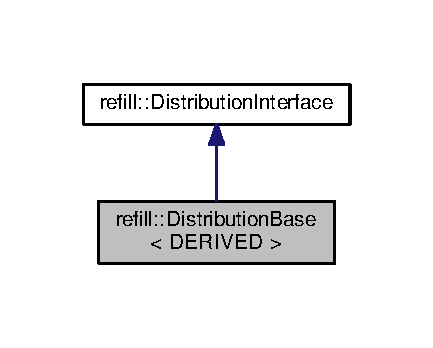
\includegraphics[width=208pt]{classrefill_1_1DistributionBase__inherit__graph}
\end{center}
\end{figure}


Collaboration diagram for refill\+:\+:Distribution\+Base$<$ D\+E\+R\+I\+V\+ED $>$\+:\nopagebreak
\begin{figure}[H]
\begin{center}
\leavevmode
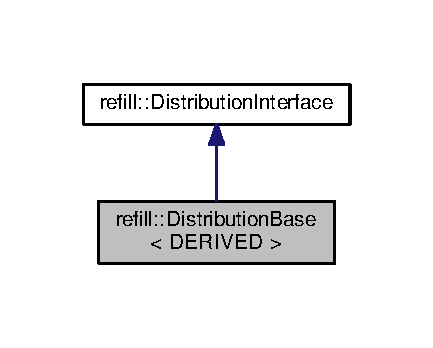
\includegraphics[width=208pt]{classrefill_1_1DistributionBase__coll__graph}
\end{center}
\end{figure}
\subsection*{Additional Inherited Members}


\subsection{Detailed Description}
\subsubsection*{template$<$typename D\+E\+R\+I\+V\+ED$>$\\*
class refill\+::\+Distribution\+Base$<$ D\+E\+R\+I\+V\+E\+D $>$}

Class that implements the C\+R\+TP. 

Class that implements the Curiously Recurring Templating Pattern so the clone function doesn\textquotesingle{}t have to be implemented in every derived distribution.

For new distributions, inherit from this class like this\+:

{\ttfamily class New\+Distribution \+: public \hyperlink{classrefill_1_1DistributionBase}{Distribution\+Base}$<$New\+Distribution$>$} 

The documentation for this class was generated from the following file\+:\begin{DoxyCompactItemize}
\item 
/home/jakob/ros/catkin\+\_\+ws/src/refill/include/refill/distributions/\hyperlink{distribution__base_8h}{distribution\+\_\+base.\+h}\end{DoxyCompactItemize}

\hypertarget{classrefill_1_1DistributionInterface}{}\section{refill\+:\+:Distribution\+Interface Class Reference}
\label{classrefill_1_1DistributionInterface}\index{refill\+::\+Distribution\+Interface@{refill\+::\+Distribution\+Interface}}


Interface for distributions.  




{\ttfamily \#include $<$distribution\+\_\+base.\+h$>$}



Inheritance diagram for refill\+:\+:Distribution\+Interface\+:\nopagebreak
\begin{figure}[H]
\begin{center}
\leavevmode
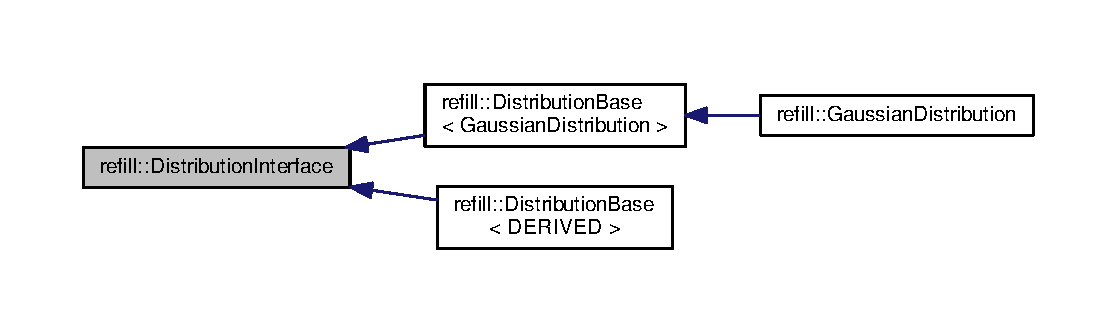
\includegraphics[width=350pt]{classrefill_1_1DistributionInterface__inherit__graph}
\end{center}
\end{figure}
\subsection*{Public Member Functions}
\begin{DoxyCompactItemize}
\item 
virtual Eigen\+::\+Vector\+Xd \hyperlink{classrefill_1_1DistributionInterface_a040f74b619ff493250e43699d7f88a5b}{mean} () const =0
\begin{DoxyCompactList}\small\item\em Returns the mean of the distribution. \end{DoxyCompactList}\item 
virtual Eigen\+::\+Matrix\+Xd \hyperlink{classrefill_1_1DistributionInterface_a88cd04a3fd67fa1702e243087c8dffa3}{cov} () const =0
\begin{DoxyCompactList}\small\item\em Returns the covariance matrix of the distribution. \end{DoxyCompactList}\item 
virtual \hyperlink{classrefill_1_1DistributionInterface}{Distribution\+Interface} $\ast$ \hyperlink{classrefill_1_1DistributionInterface_addb2d3052afd3cf114a94a3f097fae80}{clone} () const =0
\begin{DoxyCompactList}\small\item\em Clones the original distribution. \end{DoxyCompactList}\end{DoxyCompactItemize}


\subsection{Detailed Description}
Interface for distributions. 

Interface that should be used for defining new distributions. 

\subsection{Member Function Documentation}
\index{refill\+::\+Distribution\+Interface@{refill\+::\+Distribution\+Interface}!clone@{clone}}
\index{clone@{clone}!refill\+::\+Distribution\+Interface@{refill\+::\+Distribution\+Interface}}
\subsubsection[{\texorpdfstring{clone() const =0}{clone() const =0}}]{\setlength{\rightskip}{0pt plus 5cm}virtual {\bf Distribution\+Interface}$\ast$ refill\+::\+Distribution\+Interface\+::clone (
\begin{DoxyParamCaption}
{}
\end{DoxyParamCaption}
) const\hspace{0.3cm}{\ttfamily [pure virtual]}}\hypertarget{classrefill_1_1DistributionInterface_addb2d3052afd3cf114a94a3f097fae80}{}\label{classrefill_1_1DistributionInterface_addb2d3052afd3cf114a94a3f097fae80}


Clones the original distribution. 

\begin{DoxyReturn}{Returns}
a pointer to the cloned distribution. 
\end{DoxyReturn}
\index{refill\+::\+Distribution\+Interface@{refill\+::\+Distribution\+Interface}!cov@{cov}}
\index{cov@{cov}!refill\+::\+Distribution\+Interface@{refill\+::\+Distribution\+Interface}}
\subsubsection[{\texorpdfstring{cov() const =0}{cov() const =0}}]{\setlength{\rightskip}{0pt plus 5cm}virtual Eigen\+::\+Matrix\+Xd refill\+::\+Distribution\+Interface\+::cov (
\begin{DoxyParamCaption}
{}
\end{DoxyParamCaption}
) const\hspace{0.3cm}{\ttfamily [pure virtual]}}\hypertarget{classrefill_1_1DistributionInterface_a88cd04a3fd67fa1702e243087c8dffa3}{}\label{classrefill_1_1DistributionInterface_a88cd04a3fd67fa1702e243087c8dffa3}


Returns the covariance matrix of the distribution. 

\begin{DoxyReturn}{Returns}
the covariance matrix of the distribution. 
\end{DoxyReturn}


Implemented in \hyperlink{classrefill_1_1GaussianDistribution_a45f96d0d4d5bd8da390c54b5126e4072}{refill\+::\+Gaussian\+Distribution}.

\index{refill\+::\+Distribution\+Interface@{refill\+::\+Distribution\+Interface}!mean@{mean}}
\index{mean@{mean}!refill\+::\+Distribution\+Interface@{refill\+::\+Distribution\+Interface}}
\subsubsection[{\texorpdfstring{mean() const =0}{mean() const =0}}]{\setlength{\rightskip}{0pt plus 5cm}virtual Eigen\+::\+Vector\+Xd refill\+::\+Distribution\+Interface\+::mean (
\begin{DoxyParamCaption}
{}
\end{DoxyParamCaption}
) const\hspace{0.3cm}{\ttfamily [pure virtual]}}\hypertarget{classrefill_1_1DistributionInterface_a040f74b619ff493250e43699d7f88a5b}{}\label{classrefill_1_1DistributionInterface_a040f74b619ff493250e43699d7f88a5b}


Returns the mean of the distribution. 

\begin{DoxyReturn}{Returns}
mean of the distribution. 
\end{DoxyReturn}


Implemented in \hyperlink{classrefill_1_1GaussianDistribution_aa7c74dd2350c3f56877ab759cb68ba8b}{refill\+::\+Gaussian\+Distribution}.



The documentation for this class was generated from the following file\+:\begin{DoxyCompactItemize}
\item 
/home/jakob/ros/catkin\+\_\+ws/src/refill/include/refill/distributions/\hyperlink{distribution__base_8h}{distribution\+\_\+base.\+h}\end{DoxyCompactItemize}

\hypertarget{classrefill_1_1ExtendedKalmanFilter}{}\section{refill\+:\+:Extended\+Kalman\+Filter Class Reference}
\label{classrefill_1_1ExtendedKalmanFilter}\index{refill\+::\+Extended\+Kalman\+Filter@{refill\+::\+Extended\+Kalman\+Filter}}


{\ttfamily \#include $<$extended\+\_\+kalman\+\_\+filter.\+h$>$}



Inheritance diagram for refill\+:\+:Extended\+Kalman\+Filter\+:\nopagebreak
\begin{figure}[H]
\begin{center}
\leavevmode
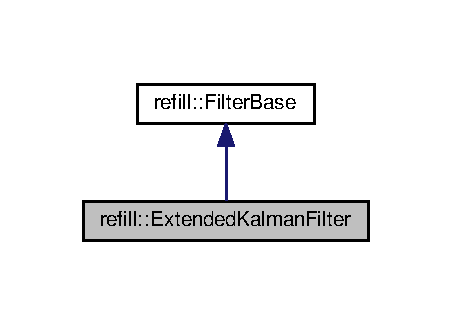
\includegraphics[width=238pt]{classrefill_1_1ExtendedKalmanFilter__inherit__graph}
\end{center}
\end{figure}


Collaboration diagram for refill\+:\+:Extended\+Kalman\+Filter\+:\nopagebreak
\begin{figure}[H]
\begin{center}
\leavevmode
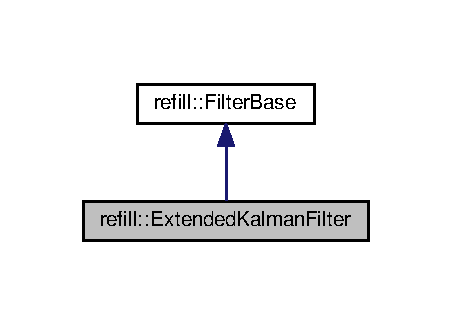
\includegraphics[width=238pt]{classrefill_1_1ExtendedKalmanFilter__coll__graph}
\end{center}
\end{figure}
\subsection*{Public Member Functions}
\begin{DoxyCompactItemize}
\item 
\hyperlink{classrefill_1_1ExtendedKalmanFilter_abf91ae94c74b1c2b8867e047d0859157}{Extended\+Kalman\+Filter} ()
\item 
\hyperlink{classrefill_1_1ExtendedKalmanFilter_af6ca041395079f69d8d32ea7376bdac5}{Extended\+Kalman\+Filter} (const \hyperlink{classrefill_1_1GaussianDistribution}{Gaussian\+Distribution} \&initial\+\_\+state)
\item 
void \hyperlink{classrefill_1_1ExtendedKalmanFilter_a10ebb05351e9e18a460e1fce35ba479a}{set\+State} (const \hyperlink{classrefill_1_1GaussianDistribution}{Gaussian\+Distribution} \&\hyperlink{classrefill_1_1ExtendedKalmanFilter_a7a8f223486039d0232e6c9d0d10b25d3}{state})
\item 
void \hyperlink{classrefill_1_1ExtendedKalmanFilter_a186407ebdf927d7a498a3e9a78a15ffc}{predict} (const \hyperlink{classrefill_1_1LinearizedSystemModel}{Linearized\+System\+Model} \&system\+\_\+model)
\item 
void \hyperlink{classrefill_1_1ExtendedKalmanFilter_ae1f0a6cd50a58b8b9c482985b2c04bd7}{predict} (const \hyperlink{classrefill_1_1LinearizedSystemModel}{Linearized\+System\+Model} \&system\+\_\+model, const Eigen\+::\+Vector\+Xd \&input)
\item 
void \hyperlink{classrefill_1_1ExtendedKalmanFilter_a7d498bfa574e87ef06c30df91d74b8ea}{update} (const \hyperlink{classrefill_1_1LinearizedMeasurementModel}{Linearized\+Measurement\+Model} \&measurement\+\_\+model, const Eigen\+::\+Vector\+Xd \&measurement)
\item 
\hyperlink{classrefill_1_1GaussianDistribution}{Gaussian\+Distribution} \hyperlink{classrefill_1_1ExtendedKalmanFilter_a7a8f223486039d0232e6c9d0d10b25d3}{state} () const 
\end{DoxyCompactItemize}


\subsection{Constructor \& Destructor Documentation}
\index{refill\+::\+Extended\+Kalman\+Filter@{refill\+::\+Extended\+Kalman\+Filter}!Extended\+Kalman\+Filter@{Extended\+Kalman\+Filter}}
\index{Extended\+Kalman\+Filter@{Extended\+Kalman\+Filter}!refill\+::\+Extended\+Kalman\+Filter@{refill\+::\+Extended\+Kalman\+Filter}}
\subsubsection[{\texorpdfstring{Extended\+Kalman\+Filter()}{ExtendedKalmanFilter()}}]{\setlength{\rightskip}{0pt plus 5cm}refill\+::\+Extended\+Kalman\+Filter\+::\+Extended\+Kalman\+Filter (
\begin{DoxyParamCaption}
{}
\end{DoxyParamCaption}
)}\hypertarget{classrefill_1_1ExtendedKalmanFilter_abf91ae94c74b1c2b8867e047d0859157}{}\label{classrefill_1_1ExtendedKalmanFilter_abf91ae94c74b1c2b8867e047d0859157}
\index{refill\+::\+Extended\+Kalman\+Filter@{refill\+::\+Extended\+Kalman\+Filter}!Extended\+Kalman\+Filter@{Extended\+Kalman\+Filter}}
\index{Extended\+Kalman\+Filter@{Extended\+Kalman\+Filter}!refill\+::\+Extended\+Kalman\+Filter@{refill\+::\+Extended\+Kalman\+Filter}}
\subsubsection[{\texorpdfstring{Extended\+Kalman\+Filter(const Gaussian\+Distribution \&initial\+\_\+state)}{ExtendedKalmanFilter(const GaussianDistribution &initial_state)}}]{\setlength{\rightskip}{0pt plus 5cm}refill\+::\+Extended\+Kalman\+Filter\+::\+Extended\+Kalman\+Filter (
\begin{DoxyParamCaption}
\item[{const {\bf Gaussian\+Distribution} \&}]{initial\+\_\+state}
\end{DoxyParamCaption}
)\hspace{0.3cm}{\ttfamily [explicit]}}\hypertarget{classrefill_1_1ExtendedKalmanFilter_af6ca041395079f69d8d32ea7376bdac5}{}\label{classrefill_1_1ExtendedKalmanFilter_af6ca041395079f69d8d32ea7376bdac5}


\subsection{Member Function Documentation}
\index{refill\+::\+Extended\+Kalman\+Filter@{refill\+::\+Extended\+Kalman\+Filter}!predict@{predict}}
\index{predict@{predict}!refill\+::\+Extended\+Kalman\+Filter@{refill\+::\+Extended\+Kalman\+Filter}}
\subsubsection[{\texorpdfstring{predict(const Linearized\+System\+Model \&system\+\_\+model)}{predict(const LinearizedSystemModel &system_model)}}]{\setlength{\rightskip}{0pt plus 5cm}void refill\+::\+Extended\+Kalman\+Filter\+::predict (
\begin{DoxyParamCaption}
\item[{const {\bf Linearized\+System\+Model} \&}]{system\+\_\+model}
\end{DoxyParamCaption}
)}\hypertarget{classrefill_1_1ExtendedKalmanFilter_a186407ebdf927d7a498a3e9a78a15ffc}{}\label{classrefill_1_1ExtendedKalmanFilter_a186407ebdf927d7a498a3e9a78a15ffc}
\index{refill\+::\+Extended\+Kalman\+Filter@{refill\+::\+Extended\+Kalman\+Filter}!predict@{predict}}
\index{predict@{predict}!refill\+::\+Extended\+Kalman\+Filter@{refill\+::\+Extended\+Kalman\+Filter}}
\subsubsection[{\texorpdfstring{predict(const Linearized\+System\+Model \&system\+\_\+model, const Eigen\+::\+Vector\+Xd \&input)}{predict(const LinearizedSystemModel &system_model, const Eigen::VectorXd &input)}}]{\setlength{\rightskip}{0pt plus 5cm}void refill\+::\+Extended\+Kalman\+Filter\+::predict (
\begin{DoxyParamCaption}
\item[{const {\bf Linearized\+System\+Model} \&}]{system\+\_\+model, }
\item[{const Eigen\+::\+Vector\+Xd \&}]{input}
\end{DoxyParamCaption}
)\hspace{0.3cm}{\ttfamily [virtual]}}\hypertarget{classrefill_1_1ExtendedKalmanFilter_ae1f0a6cd50a58b8b9c482985b2c04bd7}{}\label{classrefill_1_1ExtendedKalmanFilter_ae1f0a6cd50a58b8b9c482985b2c04bd7}


Implements \hyperlink{classrefill_1_1FilterBase_aebd38bc87b2614e9f9f71b0cab2f74b8}{refill\+::\+Filter\+Base$<$ Linearized\+System\+Model, Linearized\+Measurement\+Model $>$}.

\index{refill\+::\+Extended\+Kalman\+Filter@{refill\+::\+Extended\+Kalman\+Filter}!set\+State@{set\+State}}
\index{set\+State@{set\+State}!refill\+::\+Extended\+Kalman\+Filter@{refill\+::\+Extended\+Kalman\+Filter}}
\subsubsection[{\texorpdfstring{set\+State(const Gaussian\+Distribution \&state)}{setState(const GaussianDistribution &state)}}]{\setlength{\rightskip}{0pt plus 5cm}void refill\+::\+Extended\+Kalman\+Filter\+::set\+State (
\begin{DoxyParamCaption}
\item[{const {\bf Gaussian\+Distribution} \&}]{state}
\end{DoxyParamCaption}
)}\hypertarget{classrefill_1_1ExtendedKalmanFilter_a10ebb05351e9e18a460e1fce35ba479a}{}\label{classrefill_1_1ExtendedKalmanFilter_a10ebb05351e9e18a460e1fce35ba479a}
\index{refill\+::\+Extended\+Kalman\+Filter@{refill\+::\+Extended\+Kalman\+Filter}!state@{state}}
\index{state@{state}!refill\+::\+Extended\+Kalman\+Filter@{refill\+::\+Extended\+Kalman\+Filter}}
\subsubsection[{\texorpdfstring{state() const }{state() const }}]{\setlength{\rightskip}{0pt plus 5cm}{\bf Gaussian\+Distribution} refill\+::\+Extended\+Kalman\+Filter\+::state (
\begin{DoxyParamCaption}
{}
\end{DoxyParamCaption}
) const\hspace{0.3cm}{\ttfamily [inline]}}\hypertarget{classrefill_1_1ExtendedKalmanFilter_a7a8f223486039d0232e6c9d0d10b25d3}{}\label{classrefill_1_1ExtendedKalmanFilter_a7a8f223486039d0232e6c9d0d10b25d3}
\index{refill\+::\+Extended\+Kalman\+Filter@{refill\+::\+Extended\+Kalman\+Filter}!update@{update}}
\index{update@{update}!refill\+::\+Extended\+Kalman\+Filter@{refill\+::\+Extended\+Kalman\+Filter}}
\subsubsection[{\texorpdfstring{update(const Linearized\+Measurement\+Model \&measurement\+\_\+model, const Eigen\+::\+Vector\+Xd \&measurement)}{update(const LinearizedMeasurementModel &measurement_model, const Eigen::VectorXd &measurement)}}]{\setlength{\rightskip}{0pt plus 5cm}void refill\+::\+Extended\+Kalman\+Filter\+::update (
\begin{DoxyParamCaption}
\item[{const {\bf Linearized\+Measurement\+Model} \&}]{measurement\+\_\+model, }
\item[{const Eigen\+::\+Vector\+Xd \&}]{measurement}
\end{DoxyParamCaption}
)\hspace{0.3cm}{\ttfamily [virtual]}}\hypertarget{classrefill_1_1ExtendedKalmanFilter_a7d498bfa574e87ef06c30df91d74b8ea}{}\label{classrefill_1_1ExtendedKalmanFilter_a7d498bfa574e87ef06c30df91d74b8ea}


Implements \hyperlink{classrefill_1_1FilterBase_a1f163ae39c87c5816799ef1a84714613}{refill\+::\+Filter\+Base$<$ Linearized\+System\+Model, Linearized\+Measurement\+Model $>$}.



The documentation for this class was generated from the following files\+:\begin{DoxyCompactItemize}
\item 
/home/jakob/ros/catkin\+\_\+ws/src/refill/include/refill/filters/\hyperlink{extended__kalman__filter_8h}{extended\+\_\+kalman\+\_\+filter.\+h}\item 
/home/jakob/ros/catkin\+\_\+ws/src/refill/src/filters/\hyperlink{extended__kalman__filter_8cc}{extended\+\_\+kalman\+\_\+filter.\+cc}\end{DoxyCompactItemize}

\hypertarget{classrefill_1_1FilterBase}{}\section{refill\+:\+:Filter\+Base Class Reference}
\label{classrefill_1_1FilterBase}\index{refill\+::\+Filter\+Base@{refill\+::\+Filter\+Base}}


{\ttfamily \#include $<$filter\+\_\+base.\+h$>$}



Inheritance diagram for refill\+:\+:Filter\+Base\+:\nopagebreak
\begin{figure}[H]
\begin{center}
\leavevmode
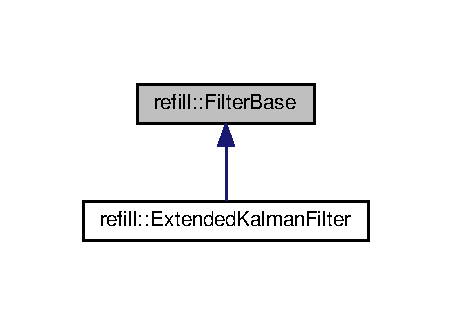
\includegraphics[width=217pt]{classrefill_1_1FilterBase__inherit__graph}
\end{center}
\end{figure}
\subsection*{Public Member Functions}
\begin{DoxyCompactItemize}
\item 
virtual void \hyperlink{classrefill_1_1FilterBase_a0f4c8d98624f222e3389f206fa1a1655}{predict} ()=0
\item 
virtual void \hyperlink{classrefill_1_1FilterBase_a24802735102854284ad9a8a78ceba8f8}{update} (const Eigen\+::\+Vector\+Xd \&measurement)=0
\end{DoxyCompactItemize}


\subsection{Member Function Documentation}
\index{refill\+::\+Filter\+Base@{refill\+::\+Filter\+Base}!predict@{predict}}
\index{predict@{predict}!refill\+::\+Filter\+Base@{refill\+::\+Filter\+Base}}
\subsubsection[{\texorpdfstring{predict()=0}{predict()=0}}]{\setlength{\rightskip}{0pt plus 5cm}virtual void refill\+::\+Filter\+Base\+::predict (
\begin{DoxyParamCaption}
{}
\end{DoxyParamCaption}
)\hspace{0.3cm}{\ttfamily [pure virtual]}}\hypertarget{classrefill_1_1FilterBase_a0f4c8d98624f222e3389f206fa1a1655}{}\label{classrefill_1_1FilterBase_a0f4c8d98624f222e3389f206fa1a1655}


Implemented in \hyperlink{classrefill_1_1ExtendedKalmanFilter_af290e17d6dba04b4dee9bdb3b5dc7f01}{refill\+::\+Extended\+Kalman\+Filter}.

\index{refill\+::\+Filter\+Base@{refill\+::\+Filter\+Base}!update@{update}}
\index{update@{update}!refill\+::\+Filter\+Base@{refill\+::\+Filter\+Base}}
\subsubsection[{\texorpdfstring{update(const Eigen\+::\+Vector\+Xd \&measurement)=0}{update(const Eigen::VectorXd &measurement)=0}}]{\setlength{\rightskip}{0pt plus 5cm}virtual void refill\+::\+Filter\+Base\+::update (
\begin{DoxyParamCaption}
\item[{const Eigen\+::\+Vector\+Xd \&}]{measurement}
\end{DoxyParamCaption}
)\hspace{0.3cm}{\ttfamily [pure virtual]}}\hypertarget{classrefill_1_1FilterBase_a24802735102854284ad9a8a78ceba8f8}{}\label{classrefill_1_1FilterBase_a24802735102854284ad9a8a78ceba8f8}


Implemented in \hyperlink{classrefill_1_1ExtendedKalmanFilter_a8d1fb40b3e129965dfa2b0aabab6d8fb}{refill\+::\+Extended\+Kalman\+Filter}.



The documentation for this class was generated from the following file\+:\begin{DoxyCompactItemize}
\item 
/home/jakob/ros/catkin\+\_\+ws/src/refill/include/refill/filters/\hyperlink{filter__base_8h}{filter\+\_\+base.\+h}\end{DoxyCompactItemize}

\hypertarget{classrefill_1_1GaussianDistribution}{}\section{refill\+:\+:Gaussian\+Distribution Class Reference}
\label{classrefill_1_1GaussianDistribution}\index{refill\+::\+Gaussian\+Distribution@{refill\+::\+Gaussian\+Distribution}}


Class that implements a multivariate Gaussian distribution.  




{\ttfamily \#include $<$gaussian\+\_\+distribution.\+h$>$}



Inheritance diagram for refill\+:\+:Gaussian\+Distribution\+:\nopagebreak
\begin{figure}[H]
\begin{center}
\leavevmode
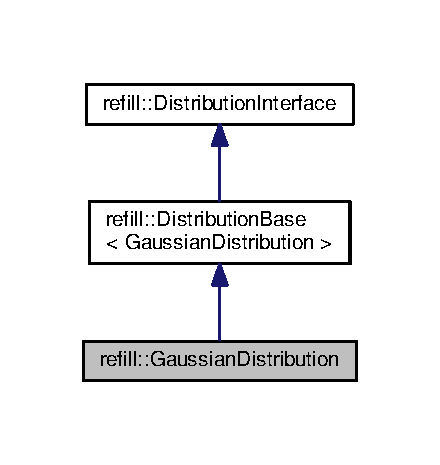
\includegraphics[width=211pt]{classrefill_1_1GaussianDistribution__inherit__graph}
\end{center}
\end{figure}


Collaboration diagram for refill\+:\+:Gaussian\+Distribution\+:\nopagebreak
\begin{figure}[H]
\begin{center}
\leavevmode
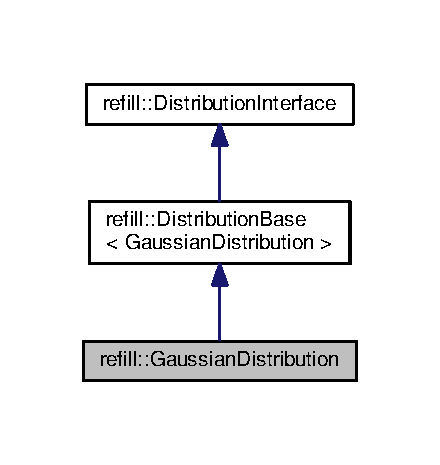
\includegraphics[width=211pt]{classrefill_1_1GaussianDistribution__coll__graph}
\end{center}
\end{figure}
\subsection*{Public Member Functions}
\begin{DoxyCompactItemize}
\item 
\hyperlink{classrefill_1_1GaussianDistribution_abca42c082cf99b5811ecf49139728f03}{Gaussian\+Distribution} ()
\begin{DoxyCompactList}\small\item\em Default constructor. \end{DoxyCompactList}\item 
\hyperlink{classrefill_1_1GaussianDistribution_aa747e7dbfa0b5bae0b0aea693436ae5a}{Gaussian\+Distribution} (const \hyperlink{classrefill_1_1GaussianDistribution}{Gaussian\+Distribution} \&dist)=default
\begin{DoxyCompactList}\small\item\em Copy constrcutor. \end{DoxyCompactList}\item 
\hyperlink{classrefill_1_1GaussianDistribution_ad90a420bb7d185f4463b07a7a1b3baf2}{Gaussian\+Distribution} (const int \&\hyperlink{classrefill_1_1GaussianDistribution_a43b275170074ef7ef38d93fb4f3e1e5a}{dimension})
\begin{DoxyCompactList}\small\item\em Constructs a normal distribution with given dimension. \end{DoxyCompactList}\item 
\hyperlink{classrefill_1_1GaussianDistribution_a2c7008059f8338e5b273637e7c13774c}{Gaussian\+Distribution} (const Eigen\+::\+Vector\+Xd \&dist\+\_\+mean, const Eigen\+::\+Matrix\+Xd \&dist\+\_\+cov)
\begin{DoxyCompactList}\small\item\em Constructs a gaussian distribution with given mean and covariance. \end{DoxyCompactList}\item 
void \hyperlink{classrefill_1_1GaussianDistribution_a2dc4f98174ef2ba08ccac80d2f85bb45}{set\+Dist\+Param} (const Eigen\+::\+Vector\+Xd \&dist\+\_\+mean, const Eigen\+::\+Matrix\+Xd \&dist\+\_\+cov)
\begin{DoxyCompactList}\small\item\em Sets the distribution parameters. \end{DoxyCompactList}\item 
void \hyperlink{classrefill_1_1GaussianDistribution_a54f8f02331947f515df30620bd6a706c}{set\+Mean} (const Eigen\+::\+Vector\+Xd \&\hyperlink{classrefill_1_1GaussianDistribution_aa7c74dd2350c3f56877ab759cb68ba8b}{mean})
\begin{DoxyCompactList}\small\item\em Sets the mean to a new value. \end{DoxyCompactList}\item 
void \hyperlink{classrefill_1_1GaussianDistribution_a48c5b06da04fef675dc044a0dabe6d86}{set\+Cov} (const Eigen\+::\+Matrix\+Xd \&\hyperlink{classrefill_1_1GaussianDistribution_a45f96d0d4d5bd8da390c54b5126e4072}{cov})
\begin{DoxyCompactList}\small\item\em Sets the covariance matrix to a new value. \end{DoxyCompactList}\item 
int \hyperlink{classrefill_1_1GaussianDistribution_a43b275170074ef7ef38d93fb4f3e1e5a}{dimension} () const 
\begin{DoxyCompactList}\small\item\em Returns the dimension of the distribution. \end{DoxyCompactList}\item 
Eigen\+::\+Vector\+Xd \hyperlink{classrefill_1_1GaussianDistribution_aa7c74dd2350c3f56877ab759cb68ba8b}{mean} () const 
\begin{DoxyCompactList}\small\item\em Returns the current mean of the distribution. \end{DoxyCompactList}\item 
Eigen\+::\+Matrix\+Xd \hyperlink{classrefill_1_1GaussianDistribution_a45f96d0d4d5bd8da390c54b5126e4072}{cov} () const 
\begin{DoxyCompactList}\small\item\em Returns the current covariance of the distribution. \end{DoxyCompactList}\item 
\hyperlink{classrefill_1_1GaussianDistribution}{Gaussian\+Distribution} \hyperlink{classrefill_1_1GaussianDistribution_aabe6056cbb9a22595e7b3b493c4f3951}{operator+} (const \hyperlink{classrefill_1_1GaussianDistribution}{Gaussian\+Distribution} \&right\+\_\+side)
\begin{DoxyCompactList}\small\item\em Implements the addition of two gaussian distributions. \end{DoxyCompactList}\end{DoxyCompactItemize}
\subsection*{Related Functions}
(Note that these are not member functions.) \begin{DoxyCompactItemize}
\item 
\hyperlink{classrefill_1_1GaussianDistribution}{Gaussian\+Distribution} \hyperlink{classrefill_1_1GaussianDistribution_a4841bb7fd2f9ea1d371d7c27a8e904aa}{operator$\ast$} (const Eigen\+::\+Matrix\+Xd \&mat, const \hyperlink{classrefill_1_1GaussianDistribution}{Gaussian\+Distribution} gaussian)
\begin{DoxyCompactList}\small\item\em Non-\/member overloaded operator for linear transformations of Gaussian random vectors. \end{DoxyCompactList}\end{DoxyCompactItemize}


\subsection{Detailed Description}
Class that implements a multivariate Gaussian distribution. 

\subsection{Constructor \& Destructor Documentation}
\index{refill\+::\+Gaussian\+Distribution@{refill\+::\+Gaussian\+Distribution}!Gaussian\+Distribution@{Gaussian\+Distribution}}
\index{Gaussian\+Distribution@{Gaussian\+Distribution}!refill\+::\+Gaussian\+Distribution@{refill\+::\+Gaussian\+Distribution}}
\subsubsection[{\texorpdfstring{Gaussian\+Distribution()}{GaussianDistribution()}}]{\setlength{\rightskip}{0pt plus 5cm}refill\+::\+Gaussian\+Distribution\+::\+Gaussian\+Distribution (
\begin{DoxyParamCaption}
{}
\end{DoxyParamCaption}
)}\hypertarget{classrefill_1_1GaussianDistribution_abca42c082cf99b5811ecf49139728f03}{}\label{classrefill_1_1GaussianDistribution_abca42c082cf99b5811ecf49139728f03}


Default constructor. 

Creates a univariate standard normal distribution. \index{refill\+::\+Gaussian\+Distribution@{refill\+::\+Gaussian\+Distribution}!Gaussian\+Distribution@{Gaussian\+Distribution}}
\index{Gaussian\+Distribution@{Gaussian\+Distribution}!refill\+::\+Gaussian\+Distribution@{refill\+::\+Gaussian\+Distribution}}
\subsubsection[{\texorpdfstring{Gaussian\+Distribution(const Gaussian\+Distribution \&dist)=default}{GaussianDistribution(const GaussianDistribution &dist)=default}}]{\setlength{\rightskip}{0pt plus 5cm}refill\+::\+Gaussian\+Distribution\+::\+Gaussian\+Distribution (
\begin{DoxyParamCaption}
\item[{const {\bf Gaussian\+Distribution} \&}]{dist}
\end{DoxyParamCaption}
)\hspace{0.3cm}{\ttfamily [default]}}\hypertarget{classrefill_1_1GaussianDistribution_aa747e7dbfa0b5bae0b0aea693436ae5a}{}\label{classrefill_1_1GaussianDistribution_aa747e7dbfa0b5bae0b0aea693436ae5a}


Copy constrcutor. 

\index{refill\+::\+Gaussian\+Distribution@{refill\+::\+Gaussian\+Distribution}!Gaussian\+Distribution@{Gaussian\+Distribution}}
\index{Gaussian\+Distribution@{Gaussian\+Distribution}!refill\+::\+Gaussian\+Distribution@{refill\+::\+Gaussian\+Distribution}}
\subsubsection[{\texorpdfstring{Gaussian\+Distribution(const int \&dimension)}{GaussianDistribution(const int &dimension)}}]{\setlength{\rightskip}{0pt plus 5cm}refill\+::\+Gaussian\+Distribution\+::\+Gaussian\+Distribution (
\begin{DoxyParamCaption}
\item[{const int \&}]{dimension}
\end{DoxyParamCaption}
)\hspace{0.3cm}{\ttfamily [explicit]}}\hypertarget{classrefill_1_1GaussianDistribution_ad90a420bb7d185f4463b07a7a1b3baf2}{}\label{classrefill_1_1GaussianDistribution_ad90a420bb7d185f4463b07a7a1b3baf2}


Constructs a normal distribution with given dimension. 


\begin{DoxyParams}{Parameters}
{\em dimension} & Dimension of the constructed normal distribution. \\
\hline
\end{DoxyParams}
\index{refill\+::\+Gaussian\+Distribution@{refill\+::\+Gaussian\+Distribution}!Gaussian\+Distribution@{Gaussian\+Distribution}}
\index{Gaussian\+Distribution@{Gaussian\+Distribution}!refill\+::\+Gaussian\+Distribution@{refill\+::\+Gaussian\+Distribution}}
\subsubsection[{\texorpdfstring{Gaussian\+Distribution(const Eigen\+::\+Vector\+Xd \&dist\+\_\+mean, const Eigen\+::\+Matrix\+Xd \&dist\+\_\+cov)}{GaussianDistribution(const Eigen::VectorXd &dist_mean, const Eigen::MatrixXd &dist_cov)}}]{\setlength{\rightskip}{0pt plus 5cm}refill\+::\+Gaussian\+Distribution\+::\+Gaussian\+Distribution (
\begin{DoxyParamCaption}
\item[{const Eigen\+::\+Vector\+Xd \&}]{dist\+\_\+mean, }
\item[{const Eigen\+::\+Matrix\+Xd \&}]{dist\+\_\+cov}
\end{DoxyParamCaption}
)}\hypertarget{classrefill_1_1GaussianDistribution_a2c7008059f8338e5b273637e7c13774c}{}\label{classrefill_1_1GaussianDistribution_a2c7008059f8338e5b273637e7c13774c}


Constructs a gaussian distribution with given mean and covariance. 


\begin{DoxyParams}{Parameters}
{\em dist\+\_\+mean} & Mean of the constructed distribution. \\
\hline
{\em dist\+\_\+cov} & Covariance matrix of the constructed distribution. \\
\hline
\end{DoxyParams}


\subsection{Member Function Documentation}
\index{refill\+::\+Gaussian\+Distribution@{refill\+::\+Gaussian\+Distribution}!cov@{cov}}
\index{cov@{cov}!refill\+::\+Gaussian\+Distribution@{refill\+::\+Gaussian\+Distribution}}
\subsubsection[{\texorpdfstring{cov() const }{cov() const }}]{\setlength{\rightskip}{0pt plus 5cm}Eigen\+::\+Matrix\+Xd refill\+::\+Gaussian\+Distribution\+::cov (
\begin{DoxyParamCaption}
{}
\end{DoxyParamCaption}
) const\hspace{0.3cm}{\ttfamily [virtual]}}\hypertarget{classrefill_1_1GaussianDistribution_a45f96d0d4d5bd8da390c54b5126e4072}{}\label{classrefill_1_1GaussianDistribution_a45f96d0d4d5bd8da390c54b5126e4072}


Returns the current covariance of the distribution. 

\begin{DoxyReturn}{Returns}
the current distribution covariance. 
\end{DoxyReturn}


Implements \hyperlink{classrefill_1_1DistributionInterface_a88cd04a3fd67fa1702e243087c8dffa3}{refill\+::\+Distribution\+Interface}.

\index{refill\+::\+Gaussian\+Distribution@{refill\+::\+Gaussian\+Distribution}!dimension@{dimension}}
\index{dimension@{dimension}!refill\+::\+Gaussian\+Distribution@{refill\+::\+Gaussian\+Distribution}}
\subsubsection[{\texorpdfstring{dimension() const }{dimension() const }}]{\setlength{\rightskip}{0pt plus 5cm}int refill\+::\+Gaussian\+Distribution\+::dimension (
\begin{DoxyParamCaption}
{}
\end{DoxyParamCaption}
) const}\hypertarget{classrefill_1_1GaussianDistribution_a43b275170074ef7ef38d93fb4f3e1e5a}{}\label{classrefill_1_1GaussianDistribution_a43b275170074ef7ef38d93fb4f3e1e5a}


Returns the dimension of the distribution. 

\begin{DoxyReturn}{Returns}
the dimension of the distribution. 
\end{DoxyReturn}
\index{refill\+::\+Gaussian\+Distribution@{refill\+::\+Gaussian\+Distribution}!mean@{mean}}
\index{mean@{mean}!refill\+::\+Gaussian\+Distribution@{refill\+::\+Gaussian\+Distribution}}
\subsubsection[{\texorpdfstring{mean() const }{mean() const }}]{\setlength{\rightskip}{0pt plus 5cm}Eigen\+::\+Vector\+Xd refill\+::\+Gaussian\+Distribution\+::mean (
\begin{DoxyParamCaption}
{}
\end{DoxyParamCaption}
) const\hspace{0.3cm}{\ttfamily [virtual]}}\hypertarget{classrefill_1_1GaussianDistribution_aa7c74dd2350c3f56877ab759cb68ba8b}{}\label{classrefill_1_1GaussianDistribution_aa7c74dd2350c3f56877ab759cb68ba8b}


Returns the current mean of the distribution. 

\begin{DoxyReturn}{Returns}
the current distribution mean. 
\end{DoxyReturn}


Implements \hyperlink{classrefill_1_1DistributionInterface_a040f74b619ff493250e43699d7f88a5b}{refill\+::\+Distribution\+Interface}.

\index{refill\+::\+Gaussian\+Distribution@{refill\+::\+Gaussian\+Distribution}!operator+@{operator+}}
\index{operator+@{operator+}!refill\+::\+Gaussian\+Distribution@{refill\+::\+Gaussian\+Distribution}}
\subsubsection[{\texorpdfstring{operator+(const Gaussian\+Distribution \&right\+\_\+side)}{operator+(const GaussianDistribution &right_side)}}]{\setlength{\rightskip}{0pt plus 5cm}{\bf Gaussian\+Distribution} refill\+::\+Gaussian\+Distribution\+::operator+ (
\begin{DoxyParamCaption}
\item[{const {\bf Gaussian\+Distribution} \&}]{right\+\_\+side}
\end{DoxyParamCaption}
)}\hypertarget{classrefill_1_1GaussianDistribution_aabe6056cbb9a22595e7b3b493c4f3951}{}\label{classrefill_1_1GaussianDistribution_aabe6056cbb9a22595e7b3b493c4f3951}


Implements the addition of two gaussian distributions. 

Checks for right dimensionality of distribution.


\begin{DoxyParams}{Parameters}
{\em right\+\_\+side} & Distribution which will be added to {\ttfamily $\ast$this}. \\
\hline
\end{DoxyParams}
\begin{DoxyReturn}{Returns}
new distribution which is the sum of {\ttfamily $\ast$this} and {\ttfamily right\+\_\+side}. 
\end{DoxyReturn}
\index{refill\+::\+Gaussian\+Distribution@{refill\+::\+Gaussian\+Distribution}!set\+Cov@{set\+Cov}}
\index{set\+Cov@{set\+Cov}!refill\+::\+Gaussian\+Distribution@{refill\+::\+Gaussian\+Distribution}}
\subsubsection[{\texorpdfstring{set\+Cov(const Eigen\+::\+Matrix\+Xd \&cov)}{setCov(const Eigen::MatrixXd &cov)}}]{\setlength{\rightskip}{0pt plus 5cm}void refill\+::\+Gaussian\+Distribution\+::set\+Cov (
\begin{DoxyParamCaption}
\item[{const Eigen\+::\+Matrix\+Xd \&}]{cov}
\end{DoxyParamCaption}
)}\hypertarget{classrefill_1_1GaussianDistribution_a48c5b06da04fef675dc044a0dabe6d86}{}\label{classrefill_1_1GaussianDistribution_a48c5b06da04fef675dc044a0dabe6d86}


Sets the covariance matrix to a new value. 

Also checks that the covariance matrix is a square matrix with the same dimension as the mean and is symmetric positiv definite.


\begin{DoxyParams}{Parameters}
{\em cov} & The new distribution covariance. \\
\hline
\end{DoxyParams}
\index{refill\+::\+Gaussian\+Distribution@{refill\+::\+Gaussian\+Distribution}!set\+Dist\+Param@{set\+Dist\+Param}}
\index{set\+Dist\+Param@{set\+Dist\+Param}!refill\+::\+Gaussian\+Distribution@{refill\+::\+Gaussian\+Distribution}}
\subsubsection[{\texorpdfstring{set\+Dist\+Param(const Eigen\+::\+Vector\+Xd \&dist\+\_\+mean, const Eigen\+::\+Matrix\+Xd \&dist\+\_\+cov)}{setDistParam(const Eigen::VectorXd &dist_mean, const Eigen::MatrixXd &dist_cov)}}]{\setlength{\rightskip}{0pt plus 5cm}void refill\+::\+Gaussian\+Distribution\+::set\+Dist\+Param (
\begin{DoxyParamCaption}
\item[{const Eigen\+::\+Vector\+Xd \&}]{dist\+\_\+mean, }
\item[{const Eigen\+::\+Matrix\+Xd \&}]{dist\+\_\+cov}
\end{DoxyParamCaption}
)}\hypertarget{classrefill_1_1GaussianDistribution_a2dc4f98174ef2ba08ccac80d2f85bb45}{}\label{classrefill_1_1GaussianDistribution_a2dc4f98174ef2ba08ccac80d2f85bb45}


Sets the distribution parameters. 

Also performes checks that the mean and covariance matrix have compatible size.


\begin{DoxyParams}{Parameters}
{\em dist\+\_\+mean} & The new mean of the distribution. \\
\hline
{\em dist\+\_\+cov} & The new covariance of the distribution. \\
\hline
\end{DoxyParams}
\index{refill\+::\+Gaussian\+Distribution@{refill\+::\+Gaussian\+Distribution}!set\+Mean@{set\+Mean}}
\index{set\+Mean@{set\+Mean}!refill\+::\+Gaussian\+Distribution@{refill\+::\+Gaussian\+Distribution}}
\subsubsection[{\texorpdfstring{set\+Mean(const Eigen\+::\+Vector\+Xd \&mean)}{setMean(const Eigen::VectorXd &mean)}}]{\setlength{\rightskip}{0pt plus 5cm}void refill\+::\+Gaussian\+Distribution\+::set\+Mean (
\begin{DoxyParamCaption}
\item[{const Eigen\+::\+Vector\+Xd \&}]{mean}
\end{DoxyParamCaption}
)}\hypertarget{classrefill_1_1GaussianDistribution_a54f8f02331947f515df30620bd6a706c}{}\label{classrefill_1_1GaussianDistribution_a54f8f02331947f515df30620bd6a706c}


Sets the mean to a new value. 

Also checks that the new mean has the same dimension as the current mean.


\begin{DoxyParams}{Parameters}
{\em mean} & The new distribution mean. \\
\hline
\end{DoxyParams}


\subsection{Friends And Related Function Documentation}
\index{refill\+::\+Gaussian\+Distribution@{refill\+::\+Gaussian\+Distribution}!operator$\ast$@{operator$\ast$}}
\index{operator$\ast$@{operator$\ast$}!refill\+::\+Gaussian\+Distribution@{refill\+::\+Gaussian\+Distribution}}
\subsubsection[{\texorpdfstring{operator$\ast$(const Eigen\+::\+Matrix\+Xd \&mat, const Gaussian\+Distribution gaussian)}{operator*(const Eigen::MatrixXd &mat, const GaussianDistribution gaussian)}}]{\setlength{\rightskip}{0pt plus 5cm}{\bf Gaussian\+Distribution} operator$\ast$ (
\begin{DoxyParamCaption}
\item[{const Eigen\+::\+Matrix\+Xd \&}]{mat, }
\item[{const {\bf Gaussian\+Distribution}}]{gaussian}
\end{DoxyParamCaption}
)\hspace{0.3cm}{\ttfamily [related]}}\hypertarget{classrefill_1_1GaussianDistribution_a4841bb7fd2f9ea1d371d7c27a8e904aa}{}\label{classrefill_1_1GaussianDistribution_a4841bb7fd2f9ea1d371d7c27a8e904aa}


Non-\/member overloaded operator for linear transformations of Gaussian random vectors. 


\begin{DoxyParams}{Parameters}
{\em mat} & Linear transformation matrix. \\
\hline
{\em gaussian} & Gaussian random vector. \\
\hline
\end{DoxyParams}
\begin{DoxyReturn}{Returns}
transformed Gaussian random vector. 
\end{DoxyReturn}


The documentation for this class was generated from the following files\+:\begin{DoxyCompactItemize}
\item 
/home/jakob/ros/catkin\+\_\+ws/src/refill/include/refill/distributions/\hyperlink{gaussian__distribution_8h}{gaussian\+\_\+distribution.\+h}\item 
/home/jakob/ros/catkin\+\_\+ws/src/refill/src/distributions/\hyperlink{gaussian__distribution_8cc}{gaussian\+\_\+distribution.\+cc}\end{DoxyCompactItemize}

\hypertarget{classrefill_1_1LinearizedMeasurementModel}{}\section{refill\+:\+:Linearized\+Measurement\+Model Class Reference}
\label{classrefill_1_1LinearizedMeasurementModel}\index{refill\+::\+Linearized\+Measurement\+Model@{refill\+::\+Linearized\+Measurement\+Model}}


{\ttfamily \#include $<$linearized\+\_\+measurement\+\_\+model.\+h$>$}



Inheritance diagram for refill\+:\+:Linearized\+Measurement\+Model\+:\nopagebreak
\begin{figure}[H]
\begin{center}
\leavevmode
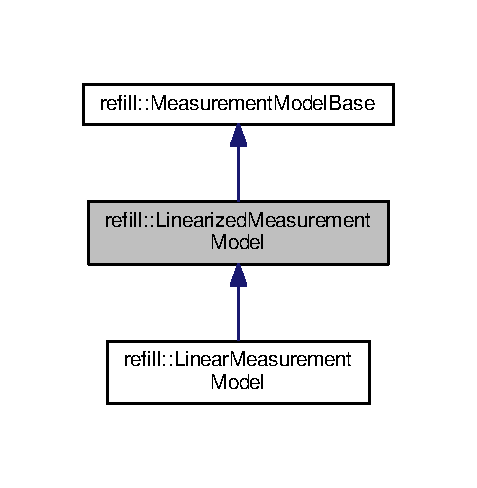
\includegraphics[width=229pt]{classrefill_1_1LinearizedMeasurementModel__inherit__graph}
\end{center}
\end{figure}


Collaboration diagram for refill\+:\+:Linearized\+Measurement\+Model\+:\nopagebreak
\begin{figure}[H]
\begin{center}
\leavevmode
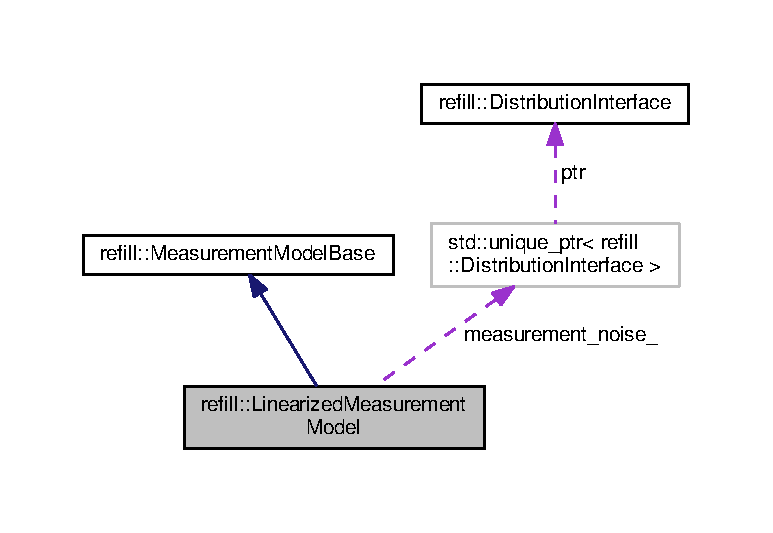
\includegraphics[width=229pt]{classrefill_1_1LinearizedMeasurementModel__coll__graph}
\end{center}
\end{figure}
\subsection*{Public Member Functions}
\begin{DoxyCompactItemize}
\item 
virtual Eigen\+::\+Matrix\+Xd \hyperlink{classrefill_1_1LinearizedMeasurementModel_a1a9fbbf32f4e71b666ee6609cdc99da7}{get\+Measurement\+Jacobian} (const Eigen\+::\+Vector\+Xd \&state) const =0
\item 
virtual Eigen\+::\+Matrix\+Xd \hyperlink{classrefill_1_1LinearizedMeasurementModel_a3573eb964dd7bff58b05af85fa46a8a0}{get\+Noise\+Jacobian} (const Eigen\+::\+Vector\+Xd \&state) const =0
\end{DoxyCompactItemize}
\subsection*{Protected Member Functions}
\begin{DoxyCompactItemize}
\item 
\hyperlink{classrefill_1_1LinearizedMeasurementModel_ac87d48f8d870169199cdb34a643c4286}{Linearized\+Measurement\+Model} ()=delete
\item 
\hyperlink{classrefill_1_1LinearizedMeasurementModel_a9acbec9c9d778a53ba395e7a2fe1ecfa}{Linearized\+Measurement\+Model} (const std\+::size\+\_\+t \&state\+\_\+dim, const std\+::size\+\_\+t \&measurement\+\_\+dim, const \hyperlink{classrefill_1_1DistributionInterface}{Distribution\+Interface} \&measurement\+\_\+noise)
\end{DoxyCompactItemize}


\subsection{Constructor \& Destructor Documentation}
\index{refill\+::\+Linearized\+Measurement\+Model@{refill\+::\+Linearized\+Measurement\+Model}!Linearized\+Measurement\+Model@{Linearized\+Measurement\+Model}}
\index{Linearized\+Measurement\+Model@{Linearized\+Measurement\+Model}!refill\+::\+Linearized\+Measurement\+Model@{refill\+::\+Linearized\+Measurement\+Model}}
\subsubsection[{\texorpdfstring{Linearized\+Measurement\+Model()=delete}{LinearizedMeasurementModel()=delete}}]{\setlength{\rightskip}{0pt plus 5cm}refill\+::\+Linearized\+Measurement\+Model\+::\+Linearized\+Measurement\+Model (
\begin{DoxyParamCaption}
{}
\end{DoxyParamCaption}
)\hspace{0.3cm}{\ttfamily [protected]}, {\ttfamily [delete]}}\hypertarget{classrefill_1_1LinearizedMeasurementModel_ac87d48f8d870169199cdb34a643c4286}{}\label{classrefill_1_1LinearizedMeasurementModel_ac87d48f8d870169199cdb34a643c4286}
\index{refill\+::\+Linearized\+Measurement\+Model@{refill\+::\+Linearized\+Measurement\+Model}!Linearized\+Measurement\+Model@{Linearized\+Measurement\+Model}}
\index{Linearized\+Measurement\+Model@{Linearized\+Measurement\+Model}!refill\+::\+Linearized\+Measurement\+Model@{refill\+::\+Linearized\+Measurement\+Model}}
\subsubsection[{\texorpdfstring{Linearized\+Measurement\+Model(const std\+::size\+\_\+t \&state\+\_\+dim, const std\+::size\+\_\+t \&measurement\+\_\+dim, const Distribution\+Interface \&measurement\+\_\+noise)}{LinearizedMeasurementModel(const std::size_t &state_dim, const std::size_t &measurement_dim, const DistributionInterface &measurement_noise)}}]{\setlength{\rightskip}{0pt plus 5cm}refill\+::\+Linearized\+Measurement\+Model\+::\+Linearized\+Measurement\+Model (
\begin{DoxyParamCaption}
\item[{const std\+::size\+\_\+t \&}]{state\+\_\+dim, }
\item[{const std\+::size\+\_\+t \&}]{measurement\+\_\+dim, }
\item[{const {\bf Distribution\+Interface} \&}]{measurement\+\_\+noise}
\end{DoxyParamCaption}
)\hspace{0.3cm}{\ttfamily [protected]}}\hypertarget{classrefill_1_1LinearizedMeasurementModel_a9acbec9c9d778a53ba395e7a2fe1ecfa}{}\label{classrefill_1_1LinearizedMeasurementModel_a9acbec9c9d778a53ba395e7a2fe1ecfa}


\subsection{Member Function Documentation}
\index{refill\+::\+Linearized\+Measurement\+Model@{refill\+::\+Linearized\+Measurement\+Model}!get\+Measurement\+Jacobian@{get\+Measurement\+Jacobian}}
\index{get\+Measurement\+Jacobian@{get\+Measurement\+Jacobian}!refill\+::\+Linearized\+Measurement\+Model@{refill\+::\+Linearized\+Measurement\+Model}}
\subsubsection[{\texorpdfstring{get\+Measurement\+Jacobian(const Eigen\+::\+Vector\+Xd \&state) const =0}{getMeasurementJacobian(const Eigen::VectorXd &state) const =0}}]{\setlength{\rightskip}{0pt plus 5cm}virtual Eigen\+::\+Matrix\+Xd refill\+::\+Linearized\+Measurement\+Model\+::get\+Measurement\+Jacobian (
\begin{DoxyParamCaption}
\item[{const Eigen\+::\+Vector\+Xd \&}]{state}
\end{DoxyParamCaption}
) const\hspace{0.3cm}{\ttfamily [pure virtual]}}\hypertarget{classrefill_1_1LinearizedMeasurementModel_a1a9fbbf32f4e71b666ee6609cdc99da7}{}\label{classrefill_1_1LinearizedMeasurementModel_a1a9fbbf32f4e71b666ee6609cdc99da7}


Implemented in \hyperlink{classrefill_1_1LinearMeasurementModel_a84f3241d0ced9d0b017b498bfed438eb}{refill\+::\+Linear\+Measurement\+Model}.

\index{refill\+::\+Linearized\+Measurement\+Model@{refill\+::\+Linearized\+Measurement\+Model}!get\+Noise\+Jacobian@{get\+Noise\+Jacobian}}
\index{get\+Noise\+Jacobian@{get\+Noise\+Jacobian}!refill\+::\+Linearized\+Measurement\+Model@{refill\+::\+Linearized\+Measurement\+Model}}
\subsubsection[{\texorpdfstring{get\+Noise\+Jacobian(const Eigen\+::\+Vector\+Xd \&state) const =0}{getNoiseJacobian(const Eigen::VectorXd &state) const =0}}]{\setlength{\rightskip}{0pt plus 5cm}virtual Eigen\+::\+Matrix\+Xd refill\+::\+Linearized\+Measurement\+Model\+::get\+Noise\+Jacobian (
\begin{DoxyParamCaption}
\item[{const Eigen\+::\+Vector\+Xd \&}]{state}
\end{DoxyParamCaption}
) const\hspace{0.3cm}{\ttfamily [pure virtual]}}\hypertarget{classrefill_1_1LinearizedMeasurementModel_a3573eb964dd7bff58b05af85fa46a8a0}{}\label{classrefill_1_1LinearizedMeasurementModel_a3573eb964dd7bff58b05af85fa46a8a0}


Implemented in \hyperlink{classrefill_1_1LinearMeasurementModel_ab31ce79fd4d2c62717443a052249f8f6}{refill\+::\+Linear\+Measurement\+Model}.



The documentation for this class was generated from the following files\+:\begin{DoxyCompactItemize}
\item 
/home/jakob/ros/catkin\+\_\+ws/src/refill/include/refill/measurement\+\_\+models/\hyperlink{linearized__measurement__model_8h}{linearized\+\_\+measurement\+\_\+model.\+h}\item 
/home/jakob/ros/catkin\+\_\+ws/src/refill/src/measurement\+\_\+models/\hyperlink{linearized__measurement__model_8cc}{linearized\+\_\+measurement\+\_\+model.\+cc}\end{DoxyCompactItemize}

\hypertarget{classrefill_1_1LinearizedSystemModel}{}\section{refill\+:\+:Linearized\+System\+Model Class Reference}
\label{classrefill_1_1LinearizedSystemModel}\index{refill\+::\+Linearized\+System\+Model@{refill\+::\+Linearized\+System\+Model}}


Class that implements a linearized system model.  




{\ttfamily \#include $<$linearized\+\_\+system\+\_\+model.\+h$>$}



Inheritance diagram for refill\+:\+:Linearized\+System\+Model\+:\nopagebreak
\begin{figure}[H]
\begin{center}
\leavevmode
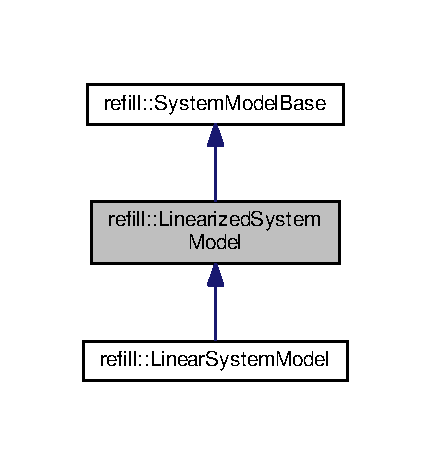
\includegraphics[width=207pt]{classrefill_1_1LinearizedSystemModel__inherit__graph}
\end{center}
\end{figure}


Collaboration diagram for refill\+:\+:Linearized\+System\+Model\+:\nopagebreak
\begin{figure}[H]
\begin{center}
\leavevmode
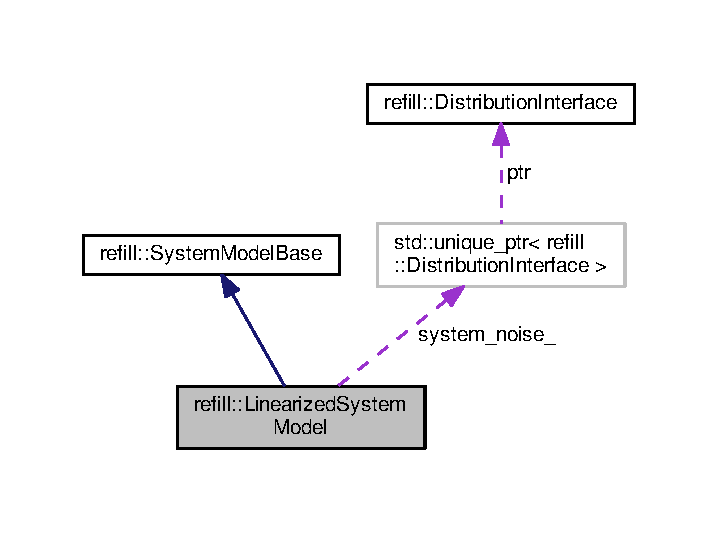
\includegraphics[width=203pt]{classrefill_1_1LinearizedSystemModel__coll__graph}
\end{center}
\end{figure}
\subsection*{Public Member Functions}
\begin{DoxyCompactItemize}
\item 
virtual Eigen\+::\+Matrix\+Xd \hyperlink{classrefill_1_1LinearizedSystemModel_a4a0bd58431d96f37cf52494fcbcd2d07}{get\+State\+Jacobian} (const Eigen\+::\+Vector\+Xd \&state, const Eigen\+::\+Vector\+Xd \&input) const =0
\begin{DoxyCompactList}\small\item\em Function to get $ A_k $, which is the system Jacobian w.\+r.\+t. the system state. \end{DoxyCompactList}\item 
virtual Eigen\+::\+Matrix\+Xd \hyperlink{classrefill_1_1LinearizedSystemModel_a2fdc435d8e47f27ad167ff31827a1c48}{get\+Noise\+Jacobian} (const Eigen\+::\+Vector\+Xd \&state, const Eigen\+::\+Vector\+Xd \&input) const =0
\begin{DoxyCompactList}\small\item\em Functoin to get $ L_k $, which is the system Jacobian w.\+r.\+t. the system noise. \end{DoxyCompactList}\end{DoxyCompactItemize}
\subsection*{Protected Member Functions}
\begin{DoxyCompactItemize}
\item 
\hyperlink{classrefill_1_1LinearizedSystemModel_aa0c5e6dea98f7d287b8b2928a42d91fe}{Linearized\+System\+Model} ()=delete
\begin{DoxyCompactList}\small\item\em Default constructor should not be used. \end{DoxyCompactList}\item 
\hyperlink{classrefill_1_1LinearizedSystemModel_a0181615604602290af776b97ed5a9200}{Linearized\+System\+Model} (const std\+::size\+\_\+t \&state\+\_\+dim, const \hyperlink{classrefill_1_1DistributionInterface}{Distribution\+Interface} \&system\+\_\+noise)
\begin{DoxyCompactList}\small\item\em Constructor for a linearized system model without an input. \end{DoxyCompactList}\item 
\hyperlink{classrefill_1_1LinearizedSystemModel_ae8b8577bdbd47e09e076580627415358}{Linearized\+System\+Model} (const std\+::size\+\_\+t \&state\+\_\+dim, const \hyperlink{classrefill_1_1DistributionInterface}{Distribution\+Interface} \&system\+\_\+noise, const std\+::size\+\_\+t \&input\+\_\+dim)
\begin{DoxyCompactList}\small\item\em Constructor for a linearized system model with an input. \end{DoxyCompactList}\end{DoxyCompactItemize}


\subsection{Detailed Description}
Class that implements a linearized system model. 

This class is an interface for system models with Jacobians.

Its intended purpose is to implement system models of the form\+:

$ x_k = f(x_{k-1}, u_k, v_k) $

With Jacobians\+:

$ A_k = \frac{\partial f}{\partial x}(x_{k-1}, u_k, \mu_k) $

and

$ L_k = \frac{\partial f}{\partial v}(x_{k-1}, u_k, \mu_k) $

Where $ x_k $ denotes the system state, $ u_k $ the system input, $ v_k $ the system noise and $ \mu_k $ the noise mean at timestep $ k $.

To implement a system model that works with the \hyperlink{classrefill_1_1ExtendedKalmanFilter}{Extended\+Kalman\+Filter}, inherit from this class and implement your own \hyperlink{classrefill_1_1SystemModelBase_a92d2c65291b3086f810e362cf4194eb0}{propagate()}, \hyperlink{classrefill_1_1LinearizedSystemModel_a4a0bd58431d96f37cf52494fcbcd2d07}{get\+State\+Jacobian()} and \hyperlink{classrefill_1_1LinearizedSystemModel_a2fdc435d8e47f27ad167ff31827a1c48}{get\+Noise\+Jacobian()} functions. 

\subsection{Constructor \& Destructor Documentation}
\index{refill\+::\+Linearized\+System\+Model@{refill\+::\+Linearized\+System\+Model}!Linearized\+System\+Model@{Linearized\+System\+Model}}
\index{Linearized\+System\+Model@{Linearized\+System\+Model}!refill\+::\+Linearized\+System\+Model@{refill\+::\+Linearized\+System\+Model}}
\subsubsection[{\texorpdfstring{Linearized\+System\+Model()=delete}{LinearizedSystemModel()=delete}}]{\setlength{\rightskip}{0pt plus 5cm}refill\+::\+Linearized\+System\+Model\+::\+Linearized\+System\+Model (
\begin{DoxyParamCaption}
{}
\end{DoxyParamCaption}
)\hspace{0.3cm}{\ttfamily [protected]}, {\ttfamily [delete]}}\hypertarget{classrefill_1_1LinearizedSystemModel_aa0c5e6dea98f7d287b8b2928a42d91fe}{}\label{classrefill_1_1LinearizedSystemModel_aa0c5e6dea98f7d287b8b2928a42d91fe}


Default constructor should not be used. 

\index{refill\+::\+Linearized\+System\+Model@{refill\+::\+Linearized\+System\+Model}!Linearized\+System\+Model@{Linearized\+System\+Model}}
\index{Linearized\+System\+Model@{Linearized\+System\+Model}!refill\+::\+Linearized\+System\+Model@{refill\+::\+Linearized\+System\+Model}}
\subsubsection[{\texorpdfstring{Linearized\+System\+Model(const std\+::size\+\_\+t \&state\+\_\+dim, const Distribution\+Interface \&system\+\_\+noise)}{LinearizedSystemModel(const std::size_t &state_dim, const DistributionInterface &system_noise)}}]{\setlength{\rightskip}{0pt plus 5cm}refill\+::\+Linearized\+System\+Model\+::\+Linearized\+System\+Model (
\begin{DoxyParamCaption}
\item[{const std\+::size\+\_\+t \&}]{state\+\_\+dim, }
\item[{const {\bf Distribution\+Interface} \&}]{system\+\_\+noise}
\end{DoxyParamCaption}
)\hspace{0.3cm}{\ttfamily [protected]}}\hypertarget{classrefill_1_1LinearizedSystemModel_a0181615604602290af776b97ed5a9200}{}\label{classrefill_1_1LinearizedSystemModel_a0181615604602290af776b97ed5a9200}


Constructor for a linearized system model without an input. 

Use this constructor if your system model does not have an input. The constructor clones the system noise, so it can be used again.


\begin{DoxyParams}{Parameters}
{\em state\+\_\+dim} & The systems state dimension. \\
\hline
{\em system\+\_\+noise} & The system noise. \\
\hline
\end{DoxyParams}
\index{refill\+::\+Linearized\+System\+Model@{refill\+::\+Linearized\+System\+Model}!Linearized\+System\+Model@{Linearized\+System\+Model}}
\index{Linearized\+System\+Model@{Linearized\+System\+Model}!refill\+::\+Linearized\+System\+Model@{refill\+::\+Linearized\+System\+Model}}
\subsubsection[{\texorpdfstring{Linearized\+System\+Model(const std\+::size\+\_\+t \&state\+\_\+dim, const Distribution\+Interface \&system\+\_\+noise, const std\+::size\+\_\+t \&input\+\_\+dim)}{LinearizedSystemModel(const std::size_t &state_dim, const DistributionInterface &system_noise, const std::size_t &input_dim)}}]{\setlength{\rightskip}{0pt plus 5cm}refill\+::\+Linearized\+System\+Model\+::\+Linearized\+System\+Model (
\begin{DoxyParamCaption}
\item[{const std\+::size\+\_\+t \&}]{state\+\_\+dim, }
\item[{const {\bf Distribution\+Interface} \&}]{system\+\_\+noise, }
\item[{const std\+::size\+\_\+t \&}]{input\+\_\+dim}
\end{DoxyParamCaption}
)\hspace{0.3cm}{\ttfamily [protected]}}\hypertarget{classrefill_1_1LinearizedSystemModel_ae8b8577bdbd47e09e076580627415358}{}\label{classrefill_1_1LinearizedSystemModel_ae8b8577bdbd47e09e076580627415358}


Constructor for a linearized system model with an input. 

Use this constructor if your system does have an input. The constructor clones the system noise, so it can be used again.


\begin{DoxyParams}{Parameters}
{\em state\+\_\+dim} & The systems state dimension. \\
\hline
{\em system\+\_\+noise} & The system noise. \\
\hline
{\em input\+\_\+dim} & The systems input dimension. \\
\hline
\end{DoxyParams}


\subsection{Member Function Documentation}
\index{refill\+::\+Linearized\+System\+Model@{refill\+::\+Linearized\+System\+Model}!get\+Noise\+Jacobian@{get\+Noise\+Jacobian}}
\index{get\+Noise\+Jacobian@{get\+Noise\+Jacobian}!refill\+::\+Linearized\+System\+Model@{refill\+::\+Linearized\+System\+Model}}
\subsubsection[{\texorpdfstring{get\+Noise\+Jacobian(const Eigen\+::\+Vector\+Xd \&state, const Eigen\+::\+Vector\+Xd \&input) const =0}{getNoiseJacobian(const Eigen::VectorXd &state, const Eigen::VectorXd &input) const =0}}]{\setlength{\rightskip}{0pt plus 5cm}virtual Eigen\+::\+Matrix\+Xd refill\+::\+Linearized\+System\+Model\+::get\+Noise\+Jacobian (
\begin{DoxyParamCaption}
\item[{const Eigen\+::\+Vector\+Xd \&}]{state, }
\item[{const Eigen\+::\+Vector\+Xd \&}]{input}
\end{DoxyParamCaption}
) const\hspace{0.3cm}{\ttfamily [pure virtual]}}\hypertarget{classrefill_1_1LinearizedSystemModel_a2fdc435d8e47f27ad167ff31827a1c48}{}\label{classrefill_1_1LinearizedSystemModel_a2fdc435d8e47f27ad167ff31827a1c48}


Functoin to get $ L_k $, which is the system Jacobian w.\+r.\+t. the system noise. 


\begin{DoxyParams}{Parameters}
{\em state} & The current system state. \\
\hline
{\em input} & The current system input. \\
\hline
\end{DoxyParams}
\begin{DoxyReturn}{Returns}
the system model Jacobian w.\+r.\+t. the system noise $v_k$. 
\end{DoxyReturn}


Implemented in \hyperlink{classrefill_1_1LinearSystemModel_ab6f766c6412db70c7fcb6676d68c1461}{refill\+::\+Linear\+System\+Model}.

\index{refill\+::\+Linearized\+System\+Model@{refill\+::\+Linearized\+System\+Model}!get\+State\+Jacobian@{get\+State\+Jacobian}}
\index{get\+State\+Jacobian@{get\+State\+Jacobian}!refill\+::\+Linearized\+System\+Model@{refill\+::\+Linearized\+System\+Model}}
\subsubsection[{\texorpdfstring{get\+State\+Jacobian(const Eigen\+::\+Vector\+Xd \&state, const Eigen\+::\+Vector\+Xd \&input) const =0}{getStateJacobian(const Eigen::VectorXd &state, const Eigen::VectorXd &input) const =0}}]{\setlength{\rightskip}{0pt plus 5cm}virtual Eigen\+::\+Matrix\+Xd refill\+::\+Linearized\+System\+Model\+::get\+State\+Jacobian (
\begin{DoxyParamCaption}
\item[{const Eigen\+::\+Vector\+Xd \&}]{state, }
\item[{const Eigen\+::\+Vector\+Xd \&}]{input}
\end{DoxyParamCaption}
) const\hspace{0.3cm}{\ttfamily [pure virtual]}}\hypertarget{classrefill_1_1LinearizedSystemModel_a4a0bd58431d96f37cf52494fcbcd2d07}{}\label{classrefill_1_1LinearizedSystemModel_a4a0bd58431d96f37cf52494fcbcd2d07}


Function to get $ A_k $, which is the system Jacobian w.\+r.\+t. the system state. 


\begin{DoxyParams}{Parameters}
{\em state} & The current system state. \\
\hline
{\em input} & The current system input. \\
\hline
\end{DoxyParams}
\begin{DoxyReturn}{Returns}
the system model Jacobian w.\+r.\+t. the system state $x_k$. 
\end{DoxyReturn}


Implemented in \hyperlink{classrefill_1_1LinearSystemModel_a165b006f5758fd0a24cec545cbfa67b6}{refill\+::\+Linear\+System\+Model}.



The documentation for this class was generated from the following files\+:\begin{DoxyCompactItemize}
\item 
/home/jakob/ros/catkin\+\_\+ws/src/refill/include/refill/system\+\_\+models/\hyperlink{linearized__system__model_8h}{linearized\+\_\+system\+\_\+model.\+h}\item 
/home/jakob/ros/catkin\+\_\+ws/src/refill/src/system\+\_\+models/\hyperlink{linearized__system__model_8cc}{linearized\+\_\+system\+\_\+model.\+cc}\end{DoxyCompactItemize}

\hypertarget{classrefill_1_1LinearMeasurementModel}{}\section{refill\+:\+:Linear\+Measurement\+Model Class Reference}
\label{classrefill_1_1LinearMeasurementModel}\index{refill\+::\+Linear\+Measurement\+Model@{refill\+::\+Linear\+Measurement\+Model}}


{\ttfamily \#include $<$linear\+\_\+measurement\+\_\+model.\+h$>$}



Inheritance diagram for refill\+:\+:Linear\+Measurement\+Model\+:\nopagebreak
\begin{figure}[H]
\begin{center}
\leavevmode
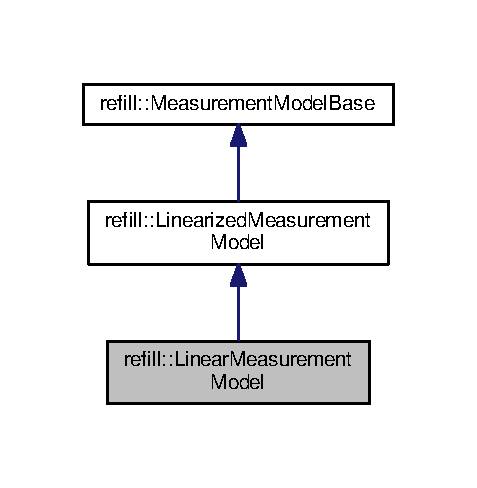
\includegraphics[width=229pt]{classrefill_1_1LinearMeasurementModel__inherit__graph}
\end{center}
\end{figure}


Collaboration diagram for refill\+:\+:Linear\+Measurement\+Model\+:\nopagebreak
\begin{figure}[H]
\begin{center}
\leavevmode
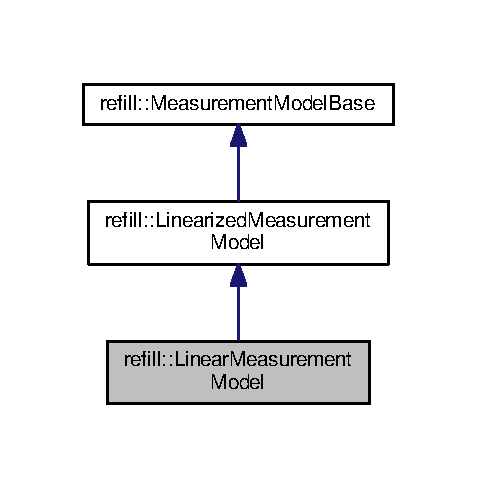
\includegraphics[width=350pt]{classrefill_1_1LinearMeasurementModel__coll__graph}
\end{center}
\end{figure}
\subsection*{Public Member Functions}
\begin{DoxyCompactItemize}
\item 
\hyperlink{classrefill_1_1LinearMeasurementModel_a90e4ff5a3fd39b3c727b389320ec1e41}{Linear\+Measurement\+Model} ()
\item 
\hyperlink{classrefill_1_1LinearMeasurementModel_ab1b3cb8e8a8e6bc1f311b9cdb96da8b7}{Linear\+Measurement\+Model} (const Eigen\+::\+Matrix\+Xd \&measurement\+\_\+mapping, const \hyperlink{classrefill_1_1DistributionInterface}{Distribution\+Interface} \&measurement\+\_\+noise)
\item 
\hyperlink{classrefill_1_1LinearMeasurementModel_a62be4c770b995a76d9ddf2b8c1e39b4b}{Linear\+Measurement\+Model} (const Eigen\+::\+Matrix\+Xd \&measurement\+\_\+mapping, const \hyperlink{classrefill_1_1DistributionInterface}{Distribution\+Interface} \&measurement\+\_\+noise, const Eigen\+::\+Matrix\+Xd \&noise\+\_\+mapping)
\item 
void \hyperlink{classrefill_1_1LinearMeasurementModel_a4086510d927ce6ad15a94fe7d4fd1a71}{set\+Measurement\+Parameters} (const Eigen\+::\+Matrix\+Xd \&measurement\+\_\+mapping, const \hyperlink{classrefill_1_1DistributionInterface}{Distribution\+Interface} \&measurement\+\_\+noise)
\item 
void \hyperlink{classrefill_1_1LinearMeasurementModel_aa514c963fd37c9aed1b2f60f833fa472}{set\+Measurement\+Parameters} (const Eigen\+::\+Matrix\+Xd \&measurement\+\_\+mapping, const \hyperlink{classrefill_1_1DistributionInterface}{Distribution\+Interface} \&measurement\+\_\+noise, const Eigen\+::\+Matrix\+Xd \&noise\+\_\+mapping)
\item 
Eigen\+::\+Vector\+Xd \hyperlink{classrefill_1_1LinearMeasurementModel_a01404c7ce5395e586738d73213c89e59}{observe} (const Eigen\+::\+Vector\+Xd \&state) const 
\item 
Eigen\+::\+Matrix\+Xd \hyperlink{classrefill_1_1LinearMeasurementModel_a84f3241d0ced9d0b017b498bfed438eb}{get\+Measurement\+Jacobian} (const Eigen\+::\+Vector\+Xd \&state) const 
\item 
Eigen\+::\+Matrix\+Xd \hyperlink{classrefill_1_1LinearMeasurementModel_ab31ce79fd4d2c62717443a052249f8f6}{get\+Noise\+Jacobian} (const Eigen\+::\+Vector\+Xd \&state) const 
\end{DoxyCompactItemize}
\subsection*{Additional Inherited Members}


\subsection{Constructor \& Destructor Documentation}
\index{refill\+::\+Linear\+Measurement\+Model@{refill\+::\+Linear\+Measurement\+Model}!Linear\+Measurement\+Model@{Linear\+Measurement\+Model}}
\index{Linear\+Measurement\+Model@{Linear\+Measurement\+Model}!refill\+::\+Linear\+Measurement\+Model@{refill\+::\+Linear\+Measurement\+Model}}
\subsubsection[{\texorpdfstring{Linear\+Measurement\+Model()}{LinearMeasurementModel()}}]{\setlength{\rightskip}{0pt plus 5cm}refill\+::\+Linear\+Measurement\+Model\+::\+Linear\+Measurement\+Model (
\begin{DoxyParamCaption}
{}
\end{DoxyParamCaption}
)}\hypertarget{classrefill_1_1LinearMeasurementModel_a90e4ff5a3fd39b3c727b389320ec1e41}{}\label{classrefill_1_1LinearMeasurementModel_a90e4ff5a3fd39b3c727b389320ec1e41}
\index{refill\+::\+Linear\+Measurement\+Model@{refill\+::\+Linear\+Measurement\+Model}!Linear\+Measurement\+Model@{Linear\+Measurement\+Model}}
\index{Linear\+Measurement\+Model@{Linear\+Measurement\+Model}!refill\+::\+Linear\+Measurement\+Model@{refill\+::\+Linear\+Measurement\+Model}}
\subsubsection[{\texorpdfstring{Linear\+Measurement\+Model(const Eigen\+::\+Matrix\+Xd \&measurement\+\_\+mapping, const Distribution\+Interface \&measurement\+\_\+noise)}{LinearMeasurementModel(const Eigen::MatrixXd &measurement_mapping, const DistributionInterface &measurement_noise)}}]{\setlength{\rightskip}{0pt plus 5cm}refill\+::\+Linear\+Measurement\+Model\+::\+Linear\+Measurement\+Model (
\begin{DoxyParamCaption}
\item[{const Eigen\+::\+Matrix\+Xd \&}]{measurement\+\_\+mapping, }
\item[{const {\bf Distribution\+Interface} \&}]{measurement\+\_\+noise}
\end{DoxyParamCaption}
)}\hypertarget{classrefill_1_1LinearMeasurementModel_ab1b3cb8e8a8e6bc1f311b9cdb96da8b7}{}\label{classrefill_1_1LinearMeasurementModel_ab1b3cb8e8a8e6bc1f311b9cdb96da8b7}
\index{refill\+::\+Linear\+Measurement\+Model@{refill\+::\+Linear\+Measurement\+Model}!Linear\+Measurement\+Model@{Linear\+Measurement\+Model}}
\index{Linear\+Measurement\+Model@{Linear\+Measurement\+Model}!refill\+::\+Linear\+Measurement\+Model@{refill\+::\+Linear\+Measurement\+Model}}
\subsubsection[{\texorpdfstring{Linear\+Measurement\+Model(const Eigen\+::\+Matrix\+Xd \&measurement\+\_\+mapping, const Distribution\+Interface \&measurement\+\_\+noise, const Eigen\+::\+Matrix\+Xd \&noise\+\_\+mapping)}{LinearMeasurementModel(const Eigen::MatrixXd &measurement_mapping, const DistributionInterface &measurement_noise, const Eigen::MatrixXd &noise_mapping)}}]{\setlength{\rightskip}{0pt plus 5cm}refill\+::\+Linear\+Measurement\+Model\+::\+Linear\+Measurement\+Model (
\begin{DoxyParamCaption}
\item[{const Eigen\+::\+Matrix\+Xd \&}]{measurement\+\_\+mapping, }
\item[{const {\bf Distribution\+Interface} \&}]{measurement\+\_\+noise, }
\item[{const Eigen\+::\+Matrix\+Xd \&}]{noise\+\_\+mapping}
\end{DoxyParamCaption}
)}\hypertarget{classrefill_1_1LinearMeasurementModel_a62be4c770b995a76d9ddf2b8c1e39b4b}{}\label{classrefill_1_1LinearMeasurementModel_a62be4c770b995a76d9ddf2b8c1e39b4b}


\subsection{Member Function Documentation}
\index{refill\+::\+Linear\+Measurement\+Model@{refill\+::\+Linear\+Measurement\+Model}!get\+Measurement\+Jacobian@{get\+Measurement\+Jacobian}}
\index{get\+Measurement\+Jacobian@{get\+Measurement\+Jacobian}!refill\+::\+Linear\+Measurement\+Model@{refill\+::\+Linear\+Measurement\+Model}}
\subsubsection[{\texorpdfstring{get\+Measurement\+Jacobian(const Eigen\+::\+Vector\+Xd \&state) const }{getMeasurementJacobian(const Eigen::VectorXd &state) const }}]{\setlength{\rightskip}{0pt plus 5cm}Eigen\+::\+Matrix\+Xd refill\+::\+Linear\+Measurement\+Model\+::get\+Measurement\+Jacobian (
\begin{DoxyParamCaption}
\item[{const Eigen\+::\+Vector\+Xd \&}]{state}
\end{DoxyParamCaption}
) const\hspace{0.3cm}{\ttfamily [virtual]}}\hypertarget{classrefill_1_1LinearMeasurementModel_a84f3241d0ced9d0b017b498bfed438eb}{}\label{classrefill_1_1LinearMeasurementModel_a84f3241d0ced9d0b017b498bfed438eb}


Implements \hyperlink{classrefill_1_1LinearizedMeasurementModel_a1a9fbbf32f4e71b666ee6609cdc99da7}{refill\+::\+Linearized\+Measurement\+Model}.

\index{refill\+::\+Linear\+Measurement\+Model@{refill\+::\+Linear\+Measurement\+Model}!get\+Noise\+Jacobian@{get\+Noise\+Jacobian}}
\index{get\+Noise\+Jacobian@{get\+Noise\+Jacobian}!refill\+::\+Linear\+Measurement\+Model@{refill\+::\+Linear\+Measurement\+Model}}
\subsubsection[{\texorpdfstring{get\+Noise\+Jacobian(const Eigen\+::\+Vector\+Xd \&state) const }{getNoiseJacobian(const Eigen::VectorXd &state) const }}]{\setlength{\rightskip}{0pt plus 5cm}Eigen\+::\+Matrix\+Xd refill\+::\+Linear\+Measurement\+Model\+::get\+Noise\+Jacobian (
\begin{DoxyParamCaption}
\item[{const Eigen\+::\+Vector\+Xd \&}]{state}
\end{DoxyParamCaption}
) const\hspace{0.3cm}{\ttfamily [virtual]}}\hypertarget{classrefill_1_1LinearMeasurementModel_ab31ce79fd4d2c62717443a052249f8f6}{}\label{classrefill_1_1LinearMeasurementModel_ab31ce79fd4d2c62717443a052249f8f6}


Implements \hyperlink{classrefill_1_1LinearizedMeasurementModel_a3573eb964dd7bff58b05af85fa46a8a0}{refill\+::\+Linearized\+Measurement\+Model}.

\index{refill\+::\+Linear\+Measurement\+Model@{refill\+::\+Linear\+Measurement\+Model}!observe@{observe}}
\index{observe@{observe}!refill\+::\+Linear\+Measurement\+Model@{refill\+::\+Linear\+Measurement\+Model}}
\subsubsection[{\texorpdfstring{observe(const Eigen\+::\+Vector\+Xd \&state) const }{observe(const Eigen::VectorXd &state) const }}]{\setlength{\rightskip}{0pt plus 5cm}Eigen\+::\+Vector\+Xd refill\+::\+Linear\+Measurement\+Model\+::observe (
\begin{DoxyParamCaption}
\item[{const Eigen\+::\+Vector\+Xd \&}]{state}
\end{DoxyParamCaption}
) const\hspace{0.3cm}{\ttfamily [virtual]}}\hypertarget{classrefill_1_1LinearMeasurementModel_a01404c7ce5395e586738d73213c89e59}{}\label{classrefill_1_1LinearMeasurementModel_a01404c7ce5395e586738d73213c89e59}


Implements \hyperlink{classrefill_1_1MeasurementModelBase_a3a5613bc1ba3317e35436fc78b0d2972}{refill\+::\+Measurement\+Model\+Base}.

\index{refill\+::\+Linear\+Measurement\+Model@{refill\+::\+Linear\+Measurement\+Model}!set\+Measurement\+Parameters@{set\+Measurement\+Parameters}}
\index{set\+Measurement\+Parameters@{set\+Measurement\+Parameters}!refill\+::\+Linear\+Measurement\+Model@{refill\+::\+Linear\+Measurement\+Model}}
\subsubsection[{\texorpdfstring{set\+Measurement\+Parameters(const Eigen\+::\+Matrix\+Xd \&measurement\+\_\+mapping, const Distribution\+Interface \&measurement\+\_\+noise)}{setMeasurementParameters(const Eigen::MatrixXd &measurement_mapping, const DistributionInterface &measurement_noise)}}]{\setlength{\rightskip}{0pt plus 5cm}void refill\+::\+Linear\+Measurement\+Model\+::set\+Measurement\+Parameters (
\begin{DoxyParamCaption}
\item[{const Eigen\+::\+Matrix\+Xd \&}]{measurement\+\_\+mapping, }
\item[{const {\bf Distribution\+Interface} \&}]{measurement\+\_\+noise}
\end{DoxyParamCaption}
)}\hypertarget{classrefill_1_1LinearMeasurementModel_a4086510d927ce6ad15a94fe7d4fd1a71}{}\label{classrefill_1_1LinearMeasurementModel_a4086510d927ce6ad15a94fe7d4fd1a71}
\index{refill\+::\+Linear\+Measurement\+Model@{refill\+::\+Linear\+Measurement\+Model}!set\+Measurement\+Parameters@{set\+Measurement\+Parameters}}
\index{set\+Measurement\+Parameters@{set\+Measurement\+Parameters}!refill\+::\+Linear\+Measurement\+Model@{refill\+::\+Linear\+Measurement\+Model}}
\subsubsection[{\texorpdfstring{set\+Measurement\+Parameters(const Eigen\+::\+Matrix\+Xd \&measurement\+\_\+mapping, const Distribution\+Interface \&measurement\+\_\+noise, const Eigen\+::\+Matrix\+Xd \&noise\+\_\+mapping)}{setMeasurementParameters(const Eigen::MatrixXd &measurement_mapping, const DistributionInterface &measurement_noise, const Eigen::MatrixXd &noise_mapping)}}]{\setlength{\rightskip}{0pt plus 5cm}void refill\+::\+Linear\+Measurement\+Model\+::set\+Measurement\+Parameters (
\begin{DoxyParamCaption}
\item[{const Eigen\+::\+Matrix\+Xd \&}]{measurement\+\_\+mapping, }
\item[{const {\bf Distribution\+Interface} \&}]{measurement\+\_\+noise, }
\item[{const Eigen\+::\+Matrix\+Xd \&}]{noise\+\_\+mapping}
\end{DoxyParamCaption}
)}\hypertarget{classrefill_1_1LinearMeasurementModel_aa514c963fd37c9aed1b2f60f833fa472}{}\label{classrefill_1_1LinearMeasurementModel_aa514c963fd37c9aed1b2f60f833fa472}


The documentation for this class was generated from the following files\+:\begin{DoxyCompactItemize}
\item 
/home/jakob/ros/catkin\+\_\+ws/src/refill/include/refill/measurement\+\_\+models/\hyperlink{linear__measurement__model_8h}{linear\+\_\+measurement\+\_\+model.\+h}\item 
/home/jakob/ros/catkin\+\_\+ws/src/refill/src/measurement\+\_\+models/\hyperlink{linear__measurement__model_8cc}{linear\+\_\+measurement\+\_\+model.\+cc}\end{DoxyCompactItemize}

\hypertarget{classrefill_1_1LinearSystemModel}{}\section{refill\+:\+:Linear\+System\+Model Class Reference}
\label{classrefill_1_1LinearSystemModel}\index{refill\+::\+Linear\+System\+Model@{refill\+::\+Linear\+System\+Model}}


{\ttfamily \#include $<$linear\+\_\+system\+\_\+model.\+h$>$}



Inheritance diagram for refill\+:\+:Linear\+System\+Model\+:\nopagebreak
\begin{figure}[H]
\begin{center}
\leavevmode
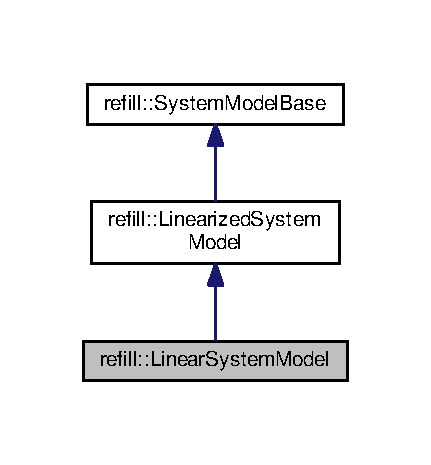
\includegraphics[width=207pt]{classrefill_1_1LinearSystemModel__inherit__graph}
\end{center}
\end{figure}


Collaboration diagram for refill\+:\+:Linear\+System\+Model\+:\nopagebreak
\begin{figure}[H]
\begin{center}
\leavevmode
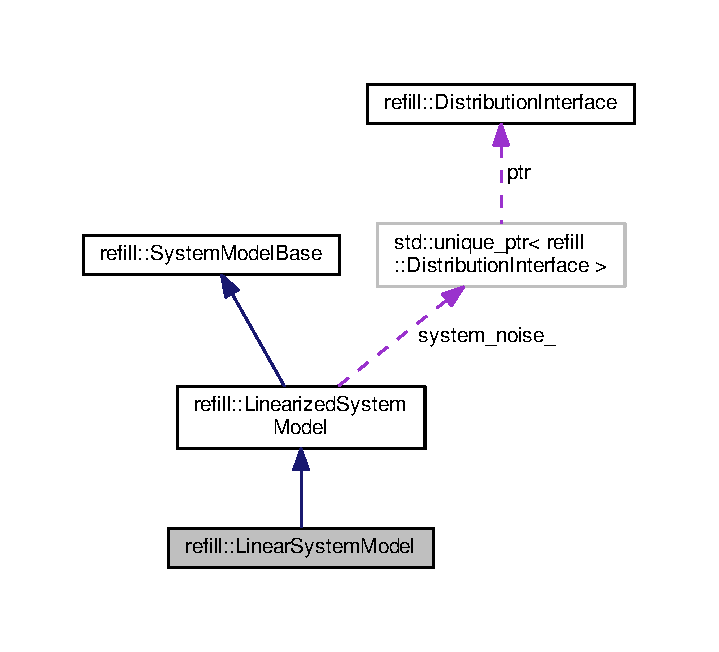
\includegraphics[width=345pt]{classrefill_1_1LinearSystemModel__coll__graph}
\end{center}
\end{figure}
\subsection*{Public Member Functions}
\begin{DoxyCompactItemize}
\item 
E\+I\+G\+E\+N\+\_\+\+M\+A\+K\+E\+\_\+\+A\+L\+I\+G\+N\+E\+D\+\_\+\+O\+P\+E\+R\+A\+T\+O\+R\+\_\+\+N\+EW \hyperlink{classrefill_1_1LinearSystemModel_a3e65d1c380d1c9abf807ca3a4814043e}{Linear\+System\+Model} ()
\item 
\hyperlink{classrefill_1_1LinearSystemModel_ab153e34ae8b09eedf442841f744851e6}{Linear\+System\+Model} (const Eigen\+::\+Matrix\+Xd \&system\+\_\+mapping, const \hyperlink{classrefill_1_1DistributionInterface}{Distribution\+Interface} \&system\+\_\+noise)
\item 
\hyperlink{classrefill_1_1LinearSystemModel_a48ede1019cfda95201e84371562d376b}{Linear\+System\+Model} (const Eigen\+::\+Matrix\+Xd \&system\+\_\+mapping, const \hyperlink{classrefill_1_1DistributionInterface}{Distribution\+Interface} \&system\+\_\+noise, const Eigen\+::\+Matrix\+Xd \&input\+\_\+mapping)
\item 
\hyperlink{classrefill_1_1LinearSystemModel_a35cfa05a9104d41f924acd5a9b183deb}{Linear\+System\+Model} (const Eigen\+::\+Matrix\+Xd \&system\+\_\+mapping, const \hyperlink{classrefill_1_1DistributionInterface}{Distribution\+Interface} \&system\+\_\+noise, const Eigen\+::\+Matrix\+Xd \&input\+\_\+mapping, const Eigen\+::\+Matrix\+Xd \&noise\+\_\+mapping)
\item 
void \hyperlink{classrefill_1_1LinearSystemModel_aa1644a0a0d363634205eaa7d1e1bfea8}{set\+System\+Parameters} (const Eigen\+::\+Matrix\+Xd \&system\+\_\+mapping, const \hyperlink{classrefill_1_1DistributionInterface}{Distribution\+Interface} \&system\+\_\+noise)
\item 
void \hyperlink{classrefill_1_1LinearSystemModel_a1bfe228bb42920399034c39ff59ae09d}{set\+System\+Parameters} (const Eigen\+::\+Matrix\+Xd \&system\+\_\+mapping, const \hyperlink{classrefill_1_1DistributionInterface}{Distribution\+Interface} \&system\+\_\+noise, const Eigen\+::\+Matrix\+Xd \&input\+\_\+mapping)
\item 
void \hyperlink{classrefill_1_1LinearSystemModel_aae2e0643e8091ccb36c14496a4e86334}{set\+System\+Parameters} (const Eigen\+::\+Matrix\+Xd \&system\+\_\+mapping, const \hyperlink{classrefill_1_1DistributionInterface}{Distribution\+Interface} \&system\+\_\+noise, const Eigen\+::\+Matrix\+Xd \&input\+\_\+mapping, const Eigen\+::\+Matrix\+Xd \&noise\+\_\+mapping)
\item 
Eigen\+::\+Vector\+Xd \hyperlink{classrefill_1_1LinearSystemModel_a6071f788057f7b1a4f382fbefd446369}{propagate} (const Eigen\+::\+Vector\+Xd \&state) const 
\item 
Eigen\+::\+Vector\+Xd \hyperlink{classrefill_1_1LinearSystemModel_a97553653a4daec3884637e1094d558ab}{propagate} (const Eigen\+::\+Vector\+Xd \&state, const Eigen\+::\+Vector\+Xd \&input) const 
\begin{DoxyCompactList}\small\item\em Propagates a state vector through the system model. \end{DoxyCompactList}\item 
Eigen\+::\+Matrix\+Xd \hyperlink{classrefill_1_1LinearSystemModel_a165b006f5758fd0a24cec545cbfa67b6}{get\+State\+Jacobian} (const Eigen\+::\+Vector\+Xd \&state, const Eigen\+::\+Vector\+Xd \&input) const 
\item 
Eigen\+::\+Matrix\+Xd \hyperlink{classrefill_1_1LinearSystemModel_ab6f766c6412db70c7fcb6676d68c1461}{get\+Noise\+Jacobian} (const Eigen\+::\+Vector\+Xd \&state, const Eigen\+::\+Vector\+Xd \&input) const 
\end{DoxyCompactItemize}
\subsection*{Additional Inherited Members}


\subsection{Constructor \& Destructor Documentation}
\index{refill\+::\+Linear\+System\+Model@{refill\+::\+Linear\+System\+Model}!Linear\+System\+Model@{Linear\+System\+Model}}
\index{Linear\+System\+Model@{Linear\+System\+Model}!refill\+::\+Linear\+System\+Model@{refill\+::\+Linear\+System\+Model}}
\subsubsection[{\texorpdfstring{Linear\+System\+Model()}{LinearSystemModel()}}]{\setlength{\rightskip}{0pt plus 5cm}refill\+::\+Linear\+System\+Model\+::\+Linear\+System\+Model (
\begin{DoxyParamCaption}
{}
\end{DoxyParamCaption}
)}\hypertarget{classrefill_1_1LinearSystemModel_a3e65d1c380d1c9abf807ca3a4814043e}{}\label{classrefill_1_1LinearSystemModel_a3e65d1c380d1c9abf807ca3a4814043e}
\index{refill\+::\+Linear\+System\+Model@{refill\+::\+Linear\+System\+Model}!Linear\+System\+Model@{Linear\+System\+Model}}
\index{Linear\+System\+Model@{Linear\+System\+Model}!refill\+::\+Linear\+System\+Model@{refill\+::\+Linear\+System\+Model}}
\subsubsection[{\texorpdfstring{Linear\+System\+Model(const Eigen\+::\+Matrix\+Xd \&system\+\_\+mapping, const Distribution\+Interface \&system\+\_\+noise)}{LinearSystemModel(const Eigen::MatrixXd &system_mapping, const DistributionInterface &system_noise)}}]{\setlength{\rightskip}{0pt plus 5cm}refill\+::\+Linear\+System\+Model\+::\+Linear\+System\+Model (
\begin{DoxyParamCaption}
\item[{const Eigen\+::\+Matrix\+Xd \&}]{system\+\_\+mapping, }
\item[{const {\bf Distribution\+Interface} \&}]{system\+\_\+noise}
\end{DoxyParamCaption}
)}\hypertarget{classrefill_1_1LinearSystemModel_ab153e34ae8b09eedf442841f744851e6}{}\label{classrefill_1_1LinearSystemModel_ab153e34ae8b09eedf442841f744851e6}
\index{refill\+::\+Linear\+System\+Model@{refill\+::\+Linear\+System\+Model}!Linear\+System\+Model@{Linear\+System\+Model}}
\index{Linear\+System\+Model@{Linear\+System\+Model}!refill\+::\+Linear\+System\+Model@{refill\+::\+Linear\+System\+Model}}
\subsubsection[{\texorpdfstring{Linear\+System\+Model(const Eigen\+::\+Matrix\+Xd \&system\+\_\+mapping, const Distribution\+Interface \&system\+\_\+noise, const Eigen\+::\+Matrix\+Xd \&input\+\_\+mapping)}{LinearSystemModel(const Eigen::MatrixXd &system_mapping, const DistributionInterface &system_noise, const Eigen::MatrixXd &input_mapping)}}]{\setlength{\rightskip}{0pt plus 5cm}refill\+::\+Linear\+System\+Model\+::\+Linear\+System\+Model (
\begin{DoxyParamCaption}
\item[{const Eigen\+::\+Matrix\+Xd \&}]{system\+\_\+mapping, }
\item[{const {\bf Distribution\+Interface} \&}]{system\+\_\+noise, }
\item[{const Eigen\+::\+Matrix\+Xd \&}]{input\+\_\+mapping}
\end{DoxyParamCaption}
)}\hypertarget{classrefill_1_1LinearSystemModel_a48ede1019cfda95201e84371562d376b}{}\label{classrefill_1_1LinearSystemModel_a48ede1019cfda95201e84371562d376b}
\index{refill\+::\+Linear\+System\+Model@{refill\+::\+Linear\+System\+Model}!Linear\+System\+Model@{Linear\+System\+Model}}
\index{Linear\+System\+Model@{Linear\+System\+Model}!refill\+::\+Linear\+System\+Model@{refill\+::\+Linear\+System\+Model}}
\subsubsection[{\texorpdfstring{Linear\+System\+Model(const Eigen\+::\+Matrix\+Xd \&system\+\_\+mapping, const Distribution\+Interface \&system\+\_\+noise, const Eigen\+::\+Matrix\+Xd \&input\+\_\+mapping, const Eigen\+::\+Matrix\+Xd \&noise\+\_\+mapping)}{LinearSystemModel(const Eigen::MatrixXd &system_mapping, const DistributionInterface &system_noise, const Eigen::MatrixXd &input_mapping, const Eigen::MatrixXd &noise_mapping)}}]{\setlength{\rightskip}{0pt plus 5cm}refill\+::\+Linear\+System\+Model\+::\+Linear\+System\+Model (
\begin{DoxyParamCaption}
\item[{const Eigen\+::\+Matrix\+Xd \&}]{system\+\_\+mapping, }
\item[{const {\bf Distribution\+Interface} \&}]{system\+\_\+noise, }
\item[{const Eigen\+::\+Matrix\+Xd \&}]{input\+\_\+mapping, }
\item[{const Eigen\+::\+Matrix\+Xd \&}]{noise\+\_\+mapping}
\end{DoxyParamCaption}
)}\hypertarget{classrefill_1_1LinearSystemModel_a35cfa05a9104d41f924acd5a9b183deb}{}\label{classrefill_1_1LinearSystemModel_a35cfa05a9104d41f924acd5a9b183deb}


\subsection{Member Function Documentation}
\index{refill\+::\+Linear\+System\+Model@{refill\+::\+Linear\+System\+Model}!get\+Noise\+Jacobian@{get\+Noise\+Jacobian}}
\index{get\+Noise\+Jacobian@{get\+Noise\+Jacobian}!refill\+::\+Linear\+System\+Model@{refill\+::\+Linear\+System\+Model}}
\subsubsection[{\texorpdfstring{get\+Noise\+Jacobian(const Eigen\+::\+Vector\+Xd \&state, const Eigen\+::\+Vector\+Xd \&input) const }{getNoiseJacobian(const Eigen::VectorXd &state, const Eigen::VectorXd &input) const }}]{\setlength{\rightskip}{0pt plus 5cm}Eigen\+::\+Matrix\+Xd refill\+::\+Linear\+System\+Model\+::get\+Noise\+Jacobian (
\begin{DoxyParamCaption}
\item[{const Eigen\+::\+Vector\+Xd \&}]{state, }
\item[{const Eigen\+::\+Vector\+Xd \&}]{input}
\end{DoxyParamCaption}
) const\hspace{0.3cm}{\ttfamily [virtual]}}\hypertarget{classrefill_1_1LinearSystemModel_ab6f766c6412db70c7fcb6676d68c1461}{}\label{classrefill_1_1LinearSystemModel_ab6f766c6412db70c7fcb6676d68c1461}


Implements \hyperlink{classrefill_1_1LinearizedSystemModel_a2fdc435d8e47f27ad167ff31827a1c48}{refill\+::\+Linearized\+System\+Model}.

\index{refill\+::\+Linear\+System\+Model@{refill\+::\+Linear\+System\+Model}!get\+State\+Jacobian@{get\+State\+Jacobian}}
\index{get\+State\+Jacobian@{get\+State\+Jacobian}!refill\+::\+Linear\+System\+Model@{refill\+::\+Linear\+System\+Model}}
\subsubsection[{\texorpdfstring{get\+State\+Jacobian(const Eigen\+::\+Vector\+Xd \&state, const Eigen\+::\+Vector\+Xd \&input) const }{getStateJacobian(const Eigen::VectorXd &state, const Eigen::VectorXd &input) const }}]{\setlength{\rightskip}{0pt plus 5cm}Eigen\+::\+Matrix\+Xd refill\+::\+Linear\+System\+Model\+::get\+State\+Jacobian (
\begin{DoxyParamCaption}
\item[{const Eigen\+::\+Vector\+Xd \&}]{state, }
\item[{const Eigen\+::\+Vector\+Xd \&}]{input}
\end{DoxyParamCaption}
) const\hspace{0.3cm}{\ttfamily [virtual]}}\hypertarget{classrefill_1_1LinearSystemModel_a165b006f5758fd0a24cec545cbfa67b6}{}\label{classrefill_1_1LinearSystemModel_a165b006f5758fd0a24cec545cbfa67b6}


Implements \hyperlink{classrefill_1_1LinearizedSystemModel_a4a0bd58431d96f37cf52494fcbcd2d07}{refill\+::\+Linearized\+System\+Model}.

\index{refill\+::\+Linear\+System\+Model@{refill\+::\+Linear\+System\+Model}!propagate@{propagate}}
\index{propagate@{propagate}!refill\+::\+Linear\+System\+Model@{refill\+::\+Linear\+System\+Model}}
\subsubsection[{\texorpdfstring{propagate(const Eigen\+::\+Vector\+Xd \&state) const }{propagate(const Eigen::VectorXd &state) const }}]{\setlength{\rightskip}{0pt plus 5cm}Eigen\+::\+Vector\+Xd refill\+::\+Linear\+System\+Model\+::propagate (
\begin{DoxyParamCaption}
\item[{const Eigen\+::\+Vector\+Xd \&}]{state}
\end{DoxyParamCaption}
) const}\hypertarget{classrefill_1_1LinearSystemModel_a6071f788057f7b1a4f382fbefd446369}{}\label{classrefill_1_1LinearSystemModel_a6071f788057f7b1a4f382fbefd446369}
\index{refill\+::\+Linear\+System\+Model@{refill\+::\+Linear\+System\+Model}!propagate@{propagate}}
\index{propagate@{propagate}!refill\+::\+Linear\+System\+Model@{refill\+::\+Linear\+System\+Model}}
\subsubsection[{\texorpdfstring{propagate(const Eigen\+::\+Vector\+Xd \&state, const Eigen\+::\+Vector\+Xd \&input) const }{propagate(const Eigen::VectorXd &state, const Eigen::VectorXd &input) const }}]{\setlength{\rightskip}{0pt plus 5cm}Eigen\+::\+Vector\+Xd refill\+::\+Linear\+System\+Model\+::propagate (
\begin{DoxyParamCaption}
\item[{const Eigen\+::\+Vector\+Xd \&}]{state, }
\item[{const Eigen\+::\+Vector\+Xd \&}]{input}
\end{DoxyParamCaption}
) const\hspace{0.3cm}{\ttfamily [virtual]}}\hypertarget{classrefill_1_1LinearSystemModel_a97553653a4daec3884637e1094d558ab}{}\label{classrefill_1_1LinearSystemModel_a97553653a4daec3884637e1094d558ab}


Propagates a state vector through the system model. 


\begin{DoxyParams}{Parameters}
{\em state} & The state vector to be propagated. \\
\hline
{\em input} & The input vector to the system. \\
\hline
\end{DoxyParams}
\begin{DoxyReturn}{Returns}
the propagated state vector. 
\end{DoxyReturn}


Implements \hyperlink{classrefill_1_1SystemModelBase_a92d2c65291b3086f810e362cf4194eb0}{refill\+::\+System\+Model\+Base}.

\index{refill\+::\+Linear\+System\+Model@{refill\+::\+Linear\+System\+Model}!set\+System\+Parameters@{set\+System\+Parameters}}
\index{set\+System\+Parameters@{set\+System\+Parameters}!refill\+::\+Linear\+System\+Model@{refill\+::\+Linear\+System\+Model}}
\subsubsection[{\texorpdfstring{set\+System\+Parameters(const Eigen\+::\+Matrix\+Xd \&system\+\_\+mapping, const Distribution\+Interface \&system\+\_\+noise)}{setSystemParameters(const Eigen::MatrixXd &system_mapping, const DistributionInterface &system_noise)}}]{\setlength{\rightskip}{0pt plus 5cm}void refill\+::\+Linear\+System\+Model\+::set\+System\+Parameters (
\begin{DoxyParamCaption}
\item[{const Eigen\+::\+Matrix\+Xd \&}]{system\+\_\+mapping, }
\item[{const {\bf Distribution\+Interface} \&}]{system\+\_\+noise}
\end{DoxyParamCaption}
)}\hypertarget{classrefill_1_1LinearSystemModel_aa1644a0a0d363634205eaa7d1e1bfea8}{}\label{classrefill_1_1LinearSystemModel_aa1644a0a0d363634205eaa7d1e1bfea8}
\index{refill\+::\+Linear\+System\+Model@{refill\+::\+Linear\+System\+Model}!set\+System\+Parameters@{set\+System\+Parameters}}
\index{set\+System\+Parameters@{set\+System\+Parameters}!refill\+::\+Linear\+System\+Model@{refill\+::\+Linear\+System\+Model}}
\subsubsection[{\texorpdfstring{set\+System\+Parameters(const Eigen\+::\+Matrix\+Xd \&system\+\_\+mapping, const Distribution\+Interface \&system\+\_\+noise, const Eigen\+::\+Matrix\+Xd \&input\+\_\+mapping)}{setSystemParameters(const Eigen::MatrixXd &system_mapping, const DistributionInterface &system_noise, const Eigen::MatrixXd &input_mapping)}}]{\setlength{\rightskip}{0pt plus 5cm}void refill\+::\+Linear\+System\+Model\+::set\+System\+Parameters (
\begin{DoxyParamCaption}
\item[{const Eigen\+::\+Matrix\+Xd \&}]{system\+\_\+mapping, }
\item[{const {\bf Distribution\+Interface} \&}]{system\+\_\+noise, }
\item[{const Eigen\+::\+Matrix\+Xd \&}]{input\+\_\+mapping}
\end{DoxyParamCaption}
)}\hypertarget{classrefill_1_1LinearSystemModel_a1bfe228bb42920399034c39ff59ae09d}{}\label{classrefill_1_1LinearSystemModel_a1bfe228bb42920399034c39ff59ae09d}
\index{refill\+::\+Linear\+System\+Model@{refill\+::\+Linear\+System\+Model}!set\+System\+Parameters@{set\+System\+Parameters}}
\index{set\+System\+Parameters@{set\+System\+Parameters}!refill\+::\+Linear\+System\+Model@{refill\+::\+Linear\+System\+Model}}
\subsubsection[{\texorpdfstring{set\+System\+Parameters(const Eigen\+::\+Matrix\+Xd \&system\+\_\+mapping, const Distribution\+Interface \&system\+\_\+noise, const Eigen\+::\+Matrix\+Xd \&input\+\_\+mapping, const Eigen\+::\+Matrix\+Xd \&noise\+\_\+mapping)}{setSystemParameters(const Eigen::MatrixXd &system_mapping, const DistributionInterface &system_noise, const Eigen::MatrixXd &input_mapping, const Eigen::MatrixXd &noise_mapping)}}]{\setlength{\rightskip}{0pt plus 5cm}void refill\+::\+Linear\+System\+Model\+::set\+System\+Parameters (
\begin{DoxyParamCaption}
\item[{const Eigen\+::\+Matrix\+Xd \&}]{system\+\_\+mapping, }
\item[{const {\bf Distribution\+Interface} \&}]{system\+\_\+noise, }
\item[{const Eigen\+::\+Matrix\+Xd \&}]{input\+\_\+mapping, }
\item[{const Eigen\+::\+Matrix\+Xd \&}]{noise\+\_\+mapping}
\end{DoxyParamCaption}
)}\hypertarget{classrefill_1_1LinearSystemModel_aae2e0643e8091ccb36c14496a4e86334}{}\label{classrefill_1_1LinearSystemModel_aae2e0643e8091ccb36c14496a4e86334}


The documentation for this class was generated from the following files\+:\begin{DoxyCompactItemize}
\item 
/home/jakob/ros/catkin\+\_\+ws/src/refill/include/refill/system\+\_\+models/\hyperlink{linear__system__model_8h}{linear\+\_\+system\+\_\+model.\+h}\item 
/home/jakob/ros/catkin\+\_\+ws/src/refill/src/system\+\_\+models/\hyperlink{linear__system__model_8cc}{linear\+\_\+system\+\_\+model.\+cc}\end{DoxyCompactItemize}

\hypertarget{classrefill_1_1MeasurementModelBase}{}\section{refill\+:\+:Measurement\+Model\+Base Class Reference}
\label{classrefill_1_1MeasurementModelBase}\index{refill\+::\+Measurement\+Model\+Base@{refill\+::\+Measurement\+Model\+Base}}


Interface for measurement models.  




{\ttfamily \#include $<$measurement\+\_\+model\+\_\+base.\+h$>$}



Inheritance diagram for refill\+:\+:Measurement\+Model\+Base\+:\nopagebreak
\begin{figure}[H]
\begin{center}
\leavevmode
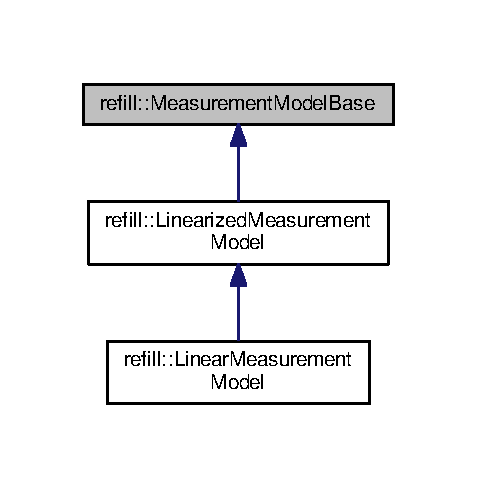
\includegraphics[width=229pt]{classrefill_1_1MeasurementModelBase__inherit__graph}
\end{center}
\end{figure}
\subsection*{Public Member Functions}
\begin{DoxyCompactItemize}
\item 
virtual Eigen\+::\+Vector\+Xd \hyperlink{classrefill_1_1MeasurementModelBase_a3a5613bc1ba3317e35436fc78b0d2972}{observe} (const Eigen\+::\+Vector\+Xd \&state) const =0
\begin{DoxyCompactList}\small\item\em Use the measurement model to receive the expected measurement. \end{DoxyCompactList}\item 
std\+::size\+\_\+t \hyperlink{classrefill_1_1MeasurementModelBase_ab87e4a5df150595abe7afcedf2b88b0f}{get\+State\+Dim} () const 
\begin{DoxyCompactList}\small\item\em Returns the measurement models state dimension. \end{DoxyCompactList}\item 
std\+::size\+\_\+t \hyperlink{classrefill_1_1MeasurementModelBase_a089b5d23a0cbbfd4ebaa02a2f2a297a9}{get\+Measurement\+Dim} () const 
\begin{DoxyCompactList}\small\item\em Returns the measurement models measurement dimension. \end{DoxyCompactList}\item 
std\+::size\+\_\+t \hyperlink{classrefill_1_1MeasurementModelBase_a0217dce62430f0888a56d7c7a4cbae28}{get\+Measurement\+Noise\+Dim} () const 
\begin{DoxyCompactList}\small\item\em Returns the measurement models noise dimension. \end{DoxyCompactList}\item 
\hyperlink{classrefill_1_1DistributionInterface}{Distribution\+Interface} $\ast$ \hyperlink{classrefill_1_1MeasurementModelBase_a3012ee640691c9b96e76168e35acdb44}{get\+Measurement\+Noise} () const 
\begin{DoxyCompactList}\small\item\em Returns the measurement models noise. \end{DoxyCompactList}\end{DoxyCompactItemize}
\subsection*{Protected Member Functions}
\begin{DoxyCompactItemize}
\item 
\hyperlink{classrefill_1_1MeasurementModelBase_a908c61f87825591b8b0f061bb5a20453}{Measurement\+Model\+Base} ()=delete
\begin{DoxyCompactList}\small\item\em Default constructor should not be used. \end{DoxyCompactList}\item 
\hyperlink{classrefill_1_1MeasurementModelBase_aecd0e5adaf05179b8fdb49c1dbb7c049}{Measurement\+Model\+Base} (const std\+::size\+\_\+t \&state\+\_\+dim, const std\+::size\+\_\+t \&measurement\+\_\+dim, const \hyperlink{classrefill_1_1DistributionInterface}{Distribution\+Interface} \&measurement\+\_\+noise)
\begin{DoxyCompactList}\small\item\em Constructor for the measurement model base class. \end{DoxyCompactList}\item 
void \hyperlink{classrefill_1_1MeasurementModelBase_aa9d94ffba2c1347dfe342865670d0185}{set\+Measurement\+Model\+Base\+Parameters} (const std\+::size\+\_\+t \&state\+\_\+dim, const std\+::size\+\_\+t \&measurement\+\_\+dim, const \hyperlink{classrefill_1_1DistributionInterface}{Distribution\+Interface} \&measurement\+\_\+noise)
\begin{DoxyCompactList}\small\item\em Function to set the measurement model base parameters. \end{DoxyCompactList}\end{DoxyCompactItemize}


\subsection{Detailed Description}
Interface for measurement models. 

All measurement models must have this class as an ancestor. 

\subsection{Constructor \& Destructor Documentation}
\index{refill\+::\+Measurement\+Model\+Base@{refill\+::\+Measurement\+Model\+Base}!Measurement\+Model\+Base@{Measurement\+Model\+Base}}
\index{Measurement\+Model\+Base@{Measurement\+Model\+Base}!refill\+::\+Measurement\+Model\+Base@{refill\+::\+Measurement\+Model\+Base}}
\subsubsection[{\texorpdfstring{Measurement\+Model\+Base()=delete}{MeasurementModelBase()=delete}}]{\setlength{\rightskip}{0pt plus 5cm}refill\+::\+Measurement\+Model\+Base\+::\+Measurement\+Model\+Base (
\begin{DoxyParamCaption}
{}
\end{DoxyParamCaption}
)\hspace{0.3cm}{\ttfamily [protected]}, {\ttfamily [delete]}}\hypertarget{classrefill_1_1MeasurementModelBase_a908c61f87825591b8b0f061bb5a20453}{}\label{classrefill_1_1MeasurementModelBase_a908c61f87825591b8b0f061bb5a20453}


Default constructor should not be used. 

\index{refill\+::\+Measurement\+Model\+Base@{refill\+::\+Measurement\+Model\+Base}!Measurement\+Model\+Base@{Measurement\+Model\+Base}}
\index{Measurement\+Model\+Base@{Measurement\+Model\+Base}!refill\+::\+Measurement\+Model\+Base@{refill\+::\+Measurement\+Model\+Base}}
\subsubsection[{\texorpdfstring{Measurement\+Model\+Base(const std\+::size\+\_\+t \&state\+\_\+dim, const std\+::size\+\_\+t \&measurement\+\_\+dim, const Distribution\+Interface \&measurement\+\_\+noise)}{MeasurementModelBase(const std::size_t &state_dim, const std::size_t &measurement_dim, const DistributionInterface &measurement_noise)}}]{\setlength{\rightskip}{0pt plus 5cm}refill\+::\+Measurement\+Model\+Base\+::\+Measurement\+Model\+Base (
\begin{DoxyParamCaption}
\item[{const std\+::size\+\_\+t \&}]{state\+\_\+dim, }
\item[{const std\+::size\+\_\+t \&}]{measurement\+\_\+dim, }
\item[{const {\bf Distribution\+Interface} \&}]{measurement\+\_\+noise}
\end{DoxyParamCaption}
)\hspace{0.3cm}{\ttfamily [protected]}}\hypertarget{classrefill_1_1MeasurementModelBase_aecd0e5adaf05179b8fdb49c1dbb7c049}{}\label{classrefill_1_1MeasurementModelBase_aecd0e5adaf05179b8fdb49c1dbb7c049}


Constructor for the measurement model base class. 

Use this constructor when inheriting from this class. The constructor clones the measurement noise, so it can be used again.


\begin{DoxyParams}{Parameters}
{\em state\+\_\+dim} & The state dimension. \\
\hline
{\em measurement\+\_\+dim} & The measurement dimension. \\
\hline
{\em measurement\+\_\+noise} & The measurement noise. \\
\hline
\end{DoxyParams}


\subsection{Member Function Documentation}
\index{refill\+::\+Measurement\+Model\+Base@{refill\+::\+Measurement\+Model\+Base}!get\+Measurement\+Dim@{get\+Measurement\+Dim}}
\index{get\+Measurement\+Dim@{get\+Measurement\+Dim}!refill\+::\+Measurement\+Model\+Base@{refill\+::\+Measurement\+Model\+Base}}
\subsubsection[{\texorpdfstring{get\+Measurement\+Dim() const }{getMeasurementDim() const }}]{\setlength{\rightskip}{0pt plus 5cm}std\+::size\+\_\+t refill\+::\+Measurement\+Model\+Base\+::get\+Measurement\+Dim (
\begin{DoxyParamCaption}
{}
\end{DoxyParamCaption}
) const}\hypertarget{classrefill_1_1MeasurementModelBase_a089b5d23a0cbbfd4ebaa02a2f2a297a9}{}\label{classrefill_1_1MeasurementModelBase_a089b5d23a0cbbfd4ebaa02a2f2a297a9}


Returns the measurement models measurement dimension. 

\begin{DoxyReturn}{Returns}
the measurement dimension. 
\end{DoxyReturn}
\index{refill\+::\+Measurement\+Model\+Base@{refill\+::\+Measurement\+Model\+Base}!get\+Measurement\+Noise@{get\+Measurement\+Noise}}
\index{get\+Measurement\+Noise@{get\+Measurement\+Noise}!refill\+::\+Measurement\+Model\+Base@{refill\+::\+Measurement\+Model\+Base}}
\subsubsection[{\texorpdfstring{get\+Measurement\+Noise() const }{getMeasurementNoise() const }}]{\setlength{\rightskip}{0pt plus 5cm}{\bf Distribution\+Interface} $\ast$ refill\+::\+Measurement\+Model\+Base\+::get\+Measurement\+Noise (
\begin{DoxyParamCaption}
{}
\end{DoxyParamCaption}
) const}\hypertarget{classrefill_1_1MeasurementModelBase_a3012ee640691c9b96e76168e35acdb44}{}\label{classrefill_1_1MeasurementModelBase_a3012ee640691c9b96e76168e35acdb44}


Returns the measurement models noise. 

\begin{DoxyReturn}{Returns}
a pointer to the measurement model noise distribution. 
\end{DoxyReturn}
\index{refill\+::\+Measurement\+Model\+Base@{refill\+::\+Measurement\+Model\+Base}!get\+Measurement\+Noise\+Dim@{get\+Measurement\+Noise\+Dim}}
\index{get\+Measurement\+Noise\+Dim@{get\+Measurement\+Noise\+Dim}!refill\+::\+Measurement\+Model\+Base@{refill\+::\+Measurement\+Model\+Base}}
\subsubsection[{\texorpdfstring{get\+Measurement\+Noise\+Dim() const }{getMeasurementNoiseDim() const }}]{\setlength{\rightskip}{0pt plus 5cm}std\+::size\+\_\+t refill\+::\+Measurement\+Model\+Base\+::get\+Measurement\+Noise\+Dim (
\begin{DoxyParamCaption}
{}
\end{DoxyParamCaption}
) const}\hypertarget{classrefill_1_1MeasurementModelBase_a0217dce62430f0888a56d7c7a4cbae28}{}\label{classrefill_1_1MeasurementModelBase_a0217dce62430f0888a56d7c7a4cbae28}


Returns the measurement models noise dimension. 

\begin{DoxyReturn}{Returns}
the noise dimension. 
\end{DoxyReturn}
\index{refill\+::\+Measurement\+Model\+Base@{refill\+::\+Measurement\+Model\+Base}!get\+State\+Dim@{get\+State\+Dim}}
\index{get\+State\+Dim@{get\+State\+Dim}!refill\+::\+Measurement\+Model\+Base@{refill\+::\+Measurement\+Model\+Base}}
\subsubsection[{\texorpdfstring{get\+State\+Dim() const }{getStateDim() const }}]{\setlength{\rightskip}{0pt plus 5cm}std\+::size\+\_\+t refill\+::\+Measurement\+Model\+Base\+::get\+State\+Dim (
\begin{DoxyParamCaption}
{}
\end{DoxyParamCaption}
) const}\hypertarget{classrefill_1_1MeasurementModelBase_ab87e4a5df150595abe7afcedf2b88b0f}{}\label{classrefill_1_1MeasurementModelBase_ab87e4a5df150595abe7afcedf2b88b0f}


Returns the measurement models state dimension. 

\begin{DoxyReturn}{Returns}
the state dimension. 
\end{DoxyReturn}
\index{refill\+::\+Measurement\+Model\+Base@{refill\+::\+Measurement\+Model\+Base}!observe@{observe}}
\index{observe@{observe}!refill\+::\+Measurement\+Model\+Base@{refill\+::\+Measurement\+Model\+Base}}
\subsubsection[{\texorpdfstring{observe(const Eigen\+::\+Vector\+Xd \&state) const =0}{observe(const Eigen::VectorXd &state) const =0}}]{\setlength{\rightskip}{0pt plus 5cm}virtual Eigen\+::\+Vector\+Xd refill\+::\+Measurement\+Model\+Base\+::observe (
\begin{DoxyParamCaption}
\item[{const Eigen\+::\+Vector\+Xd \&}]{state}
\end{DoxyParamCaption}
) const\hspace{0.3cm}{\ttfamily [pure virtual]}}\hypertarget{classrefill_1_1MeasurementModelBase_a3a5613bc1ba3317e35436fc78b0d2972}{}\label{classrefill_1_1MeasurementModelBase_a3a5613bc1ba3317e35436fc78b0d2972}


Use the measurement model to receive the expected measurement. 


\begin{DoxyParams}{Parameters}
{\em state} & The state vector used for the observation. \\
\hline
\end{DoxyParams}
\begin{DoxyReturn}{Returns}
the expected measurement given the current state. 
\end{DoxyReturn}


Implemented in \hyperlink{classrefill_1_1LinearMeasurementModel_a01404c7ce5395e586738d73213c89e59}{refill\+::\+Linear\+Measurement\+Model}.

\index{refill\+::\+Measurement\+Model\+Base@{refill\+::\+Measurement\+Model\+Base}!set\+Measurement\+Model\+Base\+Parameters@{set\+Measurement\+Model\+Base\+Parameters}}
\index{set\+Measurement\+Model\+Base\+Parameters@{set\+Measurement\+Model\+Base\+Parameters}!refill\+::\+Measurement\+Model\+Base@{refill\+::\+Measurement\+Model\+Base}}
\subsubsection[{\texorpdfstring{set\+Measurement\+Model\+Base\+Parameters(const std\+::size\+\_\+t \&state\+\_\+dim, const std\+::size\+\_\+t \&measurement\+\_\+dim, const Distribution\+Interface \&measurement\+\_\+noise)}{setMeasurementModelBaseParameters(const std::size_t &state_dim, const std::size_t &measurement_dim, const DistributionInterface &measurement_noise)}}]{\setlength{\rightskip}{0pt plus 5cm}void refill\+::\+Measurement\+Model\+Base\+::set\+Measurement\+Model\+Base\+Parameters (
\begin{DoxyParamCaption}
\item[{const std\+::size\+\_\+t \&}]{state\+\_\+dim, }
\item[{const std\+::size\+\_\+t \&}]{measurement\+\_\+dim, }
\item[{const {\bf Distribution\+Interface} \&}]{measurement\+\_\+noise}
\end{DoxyParamCaption}
)\hspace{0.3cm}{\ttfamily [protected]}}\hypertarget{classrefill_1_1MeasurementModelBase_aa9d94ffba2c1347dfe342865670d0185}{}\label{classrefill_1_1MeasurementModelBase_aa9d94ffba2c1347dfe342865670d0185}


Function to set the measurement model base parameters. 

The function clones the measurement noise, so it can be used again.


\begin{DoxyParams}{Parameters}
{\em state\+\_\+dim} & The state dimension. \\
\hline
{\em measurement\+\_\+dim} & The measurement dimension. \\
\hline
{\em measurement\+\_\+noise} & The measurement noise. \\
\hline
\end{DoxyParams}


The documentation for this class was generated from the following files\+:\begin{DoxyCompactItemize}
\item 
/home/jakob/ros/catkin\+\_\+ws/src/refill/include/refill/measurement\+\_\+models/\hyperlink{measurement__model__base_8h}{measurement\+\_\+model\+\_\+base.\+h}\item 
/home/jakob/ros/catkin\+\_\+ws/src/refill/src/measurement\+\_\+models/\hyperlink{measurement__model__base_8cc}{measurement\+\_\+model\+\_\+base.\+cc}\end{DoxyCompactItemize}

\hypertarget{classrefill_1_1SystemModelBase}{}\section{refill\+:\+:System\+Model\+Base Class Reference}
\label{classrefill_1_1SystemModelBase}\index{refill\+::\+System\+Model\+Base@{refill\+::\+System\+Model\+Base}}


Interface for system models.  




{\ttfamily \#include $<$system\+\_\+model\+\_\+base.\+h$>$}



Inheritance diagram for refill\+:\+:System\+Model\+Base\+:\nopagebreak
\begin{figure}[H]
\begin{center}
\leavevmode
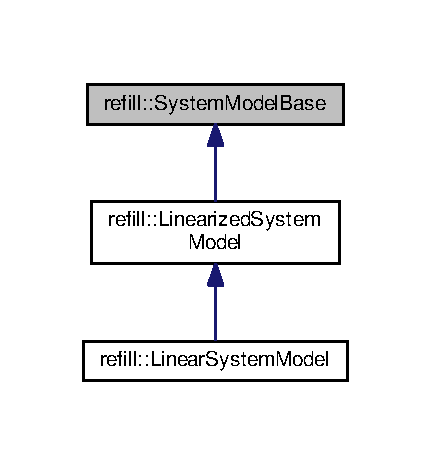
\includegraphics[width=207pt]{classrefill_1_1SystemModelBase__inherit__graph}
\end{center}
\end{figure}
\subsection*{Public Member Functions}
\begin{DoxyCompactItemize}
\item 
virtual Eigen\+::\+Vector\+Xd \hyperlink{classrefill_1_1SystemModelBase_a92d2c65291b3086f810e362cf4194eb0}{propagate} (const Eigen\+::\+Vector\+Xd \&state, const Eigen\+::\+Vector\+Xd \&input) const =0
\begin{DoxyCompactList}\small\item\em Propagates a state and input vector through the system model. \end{DoxyCompactList}\item 
std\+::size\+\_\+t \hyperlink{classrefill_1_1SystemModelBase_a56128ef3ffd3a0f4fb5ebaa543b5f719}{get\+State\+Dim} () const 
\begin{DoxyCompactList}\small\item\em Returns the systems state dimension. \end{DoxyCompactList}\item 
std\+::size\+\_\+t \hyperlink{classrefill_1_1SystemModelBase_ada4237797b93bf1da249edd2c4ec91a2}{get\+Input\+Dim} () const 
\begin{DoxyCompactList}\small\item\em Returns the systems input dimension. \end{DoxyCompactList}\item 
std\+::size\+\_\+t \hyperlink{classrefill_1_1SystemModelBase_aef4177aef8fba2c5a7c0c749c88d1c66}{get\+System\+Noise\+Dim} () const 
\begin{DoxyCompactList}\small\item\em Returns the systems noise dimension. \end{DoxyCompactList}\item 
\hyperlink{classrefill_1_1DistributionInterface}{Distribution\+Interface} $\ast$ \hyperlink{classrefill_1_1SystemModelBase_a2f733310da14248ab7f5a41840eb88b7}{get\+System\+Noise} () const 
\begin{DoxyCompactList}\small\item\em Returns a pointer to the system noise. \end{DoxyCompactList}\end{DoxyCompactItemize}
\subsection*{Protected Member Functions}
\begin{DoxyCompactItemize}
\item 
\hyperlink{classrefill_1_1SystemModelBase_a047ffd2ad50367f6015e18c316892e7f}{System\+Model\+Base} ()=delete
\item 
\hyperlink{classrefill_1_1SystemModelBase_a08f44c52bb46c5e2eb28a22f28845685}{System\+Model\+Base} (const std\+::size\+\_\+t \&state\+\_\+dim, const \hyperlink{classrefill_1_1DistributionInterface}{Distribution\+Interface} \&system\+\_\+noise)
\begin{DoxyCompactList}\small\item\em Constructor for a system model without an input. \end{DoxyCompactList}\item 
\hyperlink{classrefill_1_1SystemModelBase_a06e615416890160ecdece6a3c7511b5c}{System\+Model\+Base} (const std\+::size\+\_\+t \&state\+\_\+dim, const \hyperlink{classrefill_1_1DistributionInterface}{Distribution\+Interface} \&system\+\_\+noise, const std\+::size\+\_\+t \&input\+\_\+dim)
\begin{DoxyCompactList}\small\item\em Constructor for a system model with input. \end{DoxyCompactList}\item 
void \hyperlink{classrefill_1_1SystemModelBase_ab6aeac2bb57bdc72db21a90005ab292f}{set\+System\+Model\+Base\+Parameters} (const std\+::size\+\_\+t \&state\+\_\+dim, const \hyperlink{classrefill_1_1DistributionInterface}{Distribution\+Interface} \&system\+\_\+noise)
\begin{DoxyCompactList}\small\item\em Function to set the system model parameters without an input. \end{DoxyCompactList}\item 
void \hyperlink{classrefill_1_1SystemModelBase_a6fcf6bb1b44bfd7ccd1c0f2f1d20d53b}{set\+System\+Model\+Base\+Parameters} (const std\+::size\+\_\+t \&state\+\_\+dim, const \hyperlink{classrefill_1_1DistributionInterface}{Distribution\+Interface} \&system\+\_\+noise, const std\+::size\+\_\+t \&input\+\_\+dim)
\begin{DoxyCompactList}\small\item\em Function to set the system model parameters with an input. \end{DoxyCompactList}\end{DoxyCompactItemize}


\subsection{Detailed Description}
Interface for system models. 

All system models must have this class as an ancestor. 

\subsection{Constructor \& Destructor Documentation}
\index{refill\+::\+System\+Model\+Base@{refill\+::\+System\+Model\+Base}!System\+Model\+Base@{System\+Model\+Base}}
\index{System\+Model\+Base@{System\+Model\+Base}!refill\+::\+System\+Model\+Base@{refill\+::\+System\+Model\+Base}}
\subsubsection[{\texorpdfstring{System\+Model\+Base()=delete}{SystemModelBase()=delete}}]{\setlength{\rightskip}{0pt plus 5cm}refill\+::\+System\+Model\+Base\+::\+System\+Model\+Base (
\begin{DoxyParamCaption}
{}
\end{DoxyParamCaption}
)\hspace{0.3cm}{\ttfamily [protected]}, {\ttfamily [delete]}}\hypertarget{classrefill_1_1SystemModelBase_a047ffd2ad50367f6015e18c316892e7f}{}\label{classrefill_1_1SystemModelBase_a047ffd2ad50367f6015e18c316892e7f}
Default constructor should not be used. \index{refill\+::\+System\+Model\+Base@{refill\+::\+System\+Model\+Base}!System\+Model\+Base@{System\+Model\+Base}}
\index{System\+Model\+Base@{System\+Model\+Base}!refill\+::\+System\+Model\+Base@{refill\+::\+System\+Model\+Base}}
\subsubsection[{\texorpdfstring{System\+Model\+Base(const std\+::size\+\_\+t \&state\+\_\+dim, const Distribution\+Interface \&system\+\_\+noise)}{SystemModelBase(const std::size_t &state_dim, const DistributionInterface &system_noise)}}]{\setlength{\rightskip}{0pt plus 5cm}refill\+::\+System\+Model\+Base\+::\+System\+Model\+Base (
\begin{DoxyParamCaption}
\item[{const std\+::size\+\_\+t \&}]{state\+\_\+dim, }
\item[{const {\bf Distribution\+Interface} \&}]{system\+\_\+noise}
\end{DoxyParamCaption}
)\hspace{0.3cm}{\ttfamily [protected]}}\hypertarget{classrefill_1_1SystemModelBase_a08f44c52bb46c5e2eb28a22f28845685}{}\label{classrefill_1_1SystemModelBase_a08f44c52bb46c5e2eb28a22f28845685}


Constructor for a system model without an input. 

Use this constructor if your system does not have an input. The constructor clones the system noise, so it can be used again.


\begin{DoxyParams}{Parameters}
{\em state\+\_\+dim} & The systems state dimension. \\
\hline
{\em system\+\_\+noise} & The system noise. \\
\hline
\end{DoxyParams}
\index{refill\+::\+System\+Model\+Base@{refill\+::\+System\+Model\+Base}!System\+Model\+Base@{System\+Model\+Base}}
\index{System\+Model\+Base@{System\+Model\+Base}!refill\+::\+System\+Model\+Base@{refill\+::\+System\+Model\+Base}}
\subsubsection[{\texorpdfstring{System\+Model\+Base(const std\+::size\+\_\+t \&state\+\_\+dim, const Distribution\+Interface \&system\+\_\+noise, const std\+::size\+\_\+t \&input\+\_\+dim)}{SystemModelBase(const std::size_t &state_dim, const DistributionInterface &system_noise, const std::size_t &input_dim)}}]{\setlength{\rightskip}{0pt plus 5cm}refill\+::\+System\+Model\+Base\+::\+System\+Model\+Base (
\begin{DoxyParamCaption}
\item[{const std\+::size\+\_\+t \&}]{state\+\_\+dim, }
\item[{const {\bf Distribution\+Interface} \&}]{system\+\_\+noise, }
\item[{const std\+::size\+\_\+t \&}]{input\+\_\+dim}
\end{DoxyParamCaption}
)\hspace{0.3cm}{\ttfamily [protected]}}\hypertarget{classrefill_1_1SystemModelBase_a06e615416890160ecdece6a3c7511b5c}{}\label{classrefill_1_1SystemModelBase_a06e615416890160ecdece6a3c7511b5c}


Constructor for a system model with input. 

Use this constructor if your system model does have an input. The constructor clones the system noise, so it can be used again.


\begin{DoxyParams}{Parameters}
{\em state\+\_\+dim} & The systems state dimension. \\
\hline
{\em system\+\_\+noise} & The system noise. \\
\hline
{\em input\+\_\+dim} & The systems input dimension. \\
\hline
\end{DoxyParams}


\subsection{Member Function Documentation}
\index{refill\+::\+System\+Model\+Base@{refill\+::\+System\+Model\+Base}!get\+Input\+Dim@{get\+Input\+Dim}}
\index{get\+Input\+Dim@{get\+Input\+Dim}!refill\+::\+System\+Model\+Base@{refill\+::\+System\+Model\+Base}}
\subsubsection[{\texorpdfstring{get\+Input\+Dim() const }{getInputDim() const }}]{\setlength{\rightskip}{0pt plus 5cm}std\+::size\+\_\+t refill\+::\+System\+Model\+Base\+::get\+Input\+Dim (
\begin{DoxyParamCaption}
{}
\end{DoxyParamCaption}
) const}\hypertarget{classrefill_1_1SystemModelBase_ada4237797b93bf1da249edd2c4ec91a2}{}\label{classrefill_1_1SystemModelBase_ada4237797b93bf1da249edd2c4ec91a2}


Returns the systems input dimension. 

\begin{DoxyReturn}{Returns}
the input dimension. 
\end{DoxyReturn}
\index{refill\+::\+System\+Model\+Base@{refill\+::\+System\+Model\+Base}!get\+State\+Dim@{get\+State\+Dim}}
\index{get\+State\+Dim@{get\+State\+Dim}!refill\+::\+System\+Model\+Base@{refill\+::\+System\+Model\+Base}}
\subsubsection[{\texorpdfstring{get\+State\+Dim() const }{getStateDim() const }}]{\setlength{\rightskip}{0pt plus 5cm}std\+::size\+\_\+t refill\+::\+System\+Model\+Base\+::get\+State\+Dim (
\begin{DoxyParamCaption}
{}
\end{DoxyParamCaption}
) const}\hypertarget{classrefill_1_1SystemModelBase_a56128ef3ffd3a0f4fb5ebaa543b5f719}{}\label{classrefill_1_1SystemModelBase_a56128ef3ffd3a0f4fb5ebaa543b5f719}


Returns the systems state dimension. 

\begin{DoxyReturn}{Returns}
the state dimension. 
\end{DoxyReturn}
\index{refill\+::\+System\+Model\+Base@{refill\+::\+System\+Model\+Base}!get\+System\+Noise@{get\+System\+Noise}}
\index{get\+System\+Noise@{get\+System\+Noise}!refill\+::\+System\+Model\+Base@{refill\+::\+System\+Model\+Base}}
\subsubsection[{\texorpdfstring{get\+System\+Noise() const }{getSystemNoise() const }}]{\setlength{\rightskip}{0pt plus 5cm}{\bf Distribution\+Interface} $\ast$ refill\+::\+System\+Model\+Base\+::get\+System\+Noise (
\begin{DoxyParamCaption}
{}
\end{DoxyParamCaption}
) const}\hypertarget{classrefill_1_1SystemModelBase_a2f733310da14248ab7f5a41840eb88b7}{}\label{classrefill_1_1SystemModelBase_a2f733310da14248ab7f5a41840eb88b7}


Returns a pointer to the system noise. 

\begin{DoxyReturn}{Returns}
a pointer to the system noise distribution. 
\end{DoxyReturn}
\index{refill\+::\+System\+Model\+Base@{refill\+::\+System\+Model\+Base}!get\+System\+Noise\+Dim@{get\+System\+Noise\+Dim}}
\index{get\+System\+Noise\+Dim@{get\+System\+Noise\+Dim}!refill\+::\+System\+Model\+Base@{refill\+::\+System\+Model\+Base}}
\subsubsection[{\texorpdfstring{get\+System\+Noise\+Dim() const }{getSystemNoiseDim() const }}]{\setlength{\rightskip}{0pt plus 5cm}std\+::size\+\_\+t refill\+::\+System\+Model\+Base\+::get\+System\+Noise\+Dim (
\begin{DoxyParamCaption}
{}
\end{DoxyParamCaption}
) const}\hypertarget{classrefill_1_1SystemModelBase_aef4177aef8fba2c5a7c0c749c88d1c66}{}\label{classrefill_1_1SystemModelBase_aef4177aef8fba2c5a7c0c749c88d1c66}


Returns the systems noise dimension. 

\begin{DoxyReturn}{Returns}
the noise dimension. 
\end{DoxyReturn}
\index{refill\+::\+System\+Model\+Base@{refill\+::\+System\+Model\+Base}!propagate@{propagate}}
\index{propagate@{propagate}!refill\+::\+System\+Model\+Base@{refill\+::\+System\+Model\+Base}}
\subsubsection[{\texorpdfstring{propagate(const Eigen\+::\+Vector\+Xd \&state, const Eigen\+::\+Vector\+Xd \&input) const =0}{propagate(const Eigen::VectorXd &state, const Eigen::VectorXd &input) const =0}}]{\setlength{\rightskip}{0pt plus 5cm}virtual Eigen\+::\+Vector\+Xd refill\+::\+System\+Model\+Base\+::propagate (
\begin{DoxyParamCaption}
\item[{const Eigen\+::\+Vector\+Xd \&}]{state, }
\item[{const Eigen\+::\+Vector\+Xd \&}]{input}
\end{DoxyParamCaption}
) const\hspace{0.3cm}{\ttfamily [pure virtual]}}\hypertarget{classrefill_1_1SystemModelBase_a92d2c65291b3086f810e362cf4194eb0}{}\label{classrefill_1_1SystemModelBase_a92d2c65291b3086f810e362cf4194eb0}


Propagates a state and input vector through the system model. 


\begin{DoxyParams}{Parameters}
{\em state} & The state vector to be propagated. \\
\hline
{\em input} & The input vector to the system. \\
\hline
\end{DoxyParams}
\begin{DoxyReturn}{Returns}
the new state vector. 
\end{DoxyReturn}


Implemented in \hyperlink{classrefill_1_1LinearSystemModel_a97553653a4daec3884637e1094d558ab}{refill\+::\+Linear\+System\+Model}.

\index{refill\+::\+System\+Model\+Base@{refill\+::\+System\+Model\+Base}!set\+System\+Model\+Base\+Parameters@{set\+System\+Model\+Base\+Parameters}}
\index{set\+System\+Model\+Base\+Parameters@{set\+System\+Model\+Base\+Parameters}!refill\+::\+System\+Model\+Base@{refill\+::\+System\+Model\+Base}}
\subsubsection[{\texorpdfstring{set\+System\+Model\+Base\+Parameters(const std\+::size\+\_\+t \&state\+\_\+dim, const Distribution\+Interface \&system\+\_\+noise)}{setSystemModelBaseParameters(const std::size_t &state_dim, const DistributionInterface &system_noise)}}]{\setlength{\rightskip}{0pt plus 5cm}void refill\+::\+System\+Model\+Base\+::set\+System\+Model\+Base\+Parameters (
\begin{DoxyParamCaption}
\item[{const std\+::size\+\_\+t \&}]{state\+\_\+dim, }
\item[{const {\bf Distribution\+Interface} \&}]{system\+\_\+noise}
\end{DoxyParamCaption}
)\hspace{0.3cm}{\ttfamily [protected]}}\hypertarget{classrefill_1_1SystemModelBase_ab6aeac2bb57bdc72db21a90005ab292f}{}\label{classrefill_1_1SystemModelBase_ab6aeac2bb57bdc72db21a90005ab292f}


Function to set the system model parameters without an input. 

\index{refill\+::\+System\+Model\+Base@{refill\+::\+System\+Model\+Base}!set\+System\+Model\+Base\+Parameters@{set\+System\+Model\+Base\+Parameters}}
\index{set\+System\+Model\+Base\+Parameters@{set\+System\+Model\+Base\+Parameters}!refill\+::\+System\+Model\+Base@{refill\+::\+System\+Model\+Base}}
\subsubsection[{\texorpdfstring{set\+System\+Model\+Base\+Parameters(const std\+::size\+\_\+t \&state\+\_\+dim, const Distribution\+Interface \&system\+\_\+noise, const std\+::size\+\_\+t \&input\+\_\+dim)}{setSystemModelBaseParameters(const std::size_t &state_dim, const DistributionInterface &system_noise, const std::size_t &input_dim)}}]{\setlength{\rightskip}{0pt plus 5cm}void refill\+::\+System\+Model\+Base\+::set\+System\+Model\+Base\+Parameters (
\begin{DoxyParamCaption}
\item[{const std\+::size\+\_\+t \&}]{state\+\_\+dim, }
\item[{const {\bf Distribution\+Interface} \&}]{system\+\_\+noise, }
\item[{const std\+::size\+\_\+t \&}]{input\+\_\+dim}
\end{DoxyParamCaption}
)\hspace{0.3cm}{\ttfamily [protected]}}\hypertarget{classrefill_1_1SystemModelBase_a6fcf6bb1b44bfd7ccd1c0f2f1d20d53b}{}\label{classrefill_1_1SystemModelBase_a6fcf6bb1b44bfd7ccd1c0f2f1d20d53b}


Function to set the system model parameters with an input. 



The documentation for this class was generated from the following files\+:\begin{DoxyCompactItemize}
\item 
/home/jakob/ros/catkin\+\_\+ws/src/refill/include/refill/system\+\_\+models/\hyperlink{system__model__base_8h}{system\+\_\+model\+\_\+base.\+h}\item 
/home/jakob/ros/catkin\+\_\+ws/src/refill/src/system\+\_\+models/\hyperlink{system__model__base_8cc}{system\+\_\+model\+\_\+base.\+cc}\end{DoxyCompactItemize}

\chapter{File Documentation}
\hypertarget{distribution__base_8h}{}\section{/home/jakob/ros/catkin\+\_\+ws/src/refill/include/refill/distributions/distribution\+\_\+base.h File Reference}
\label{distribution__base_8h}\index{/home/jakob/ros/catkin\+\_\+ws/src/refill/include/refill/distributions/distribution\+\_\+base.\+h@{/home/jakob/ros/catkin\+\_\+ws/src/refill/include/refill/distributions/distribution\+\_\+base.\+h}}
{\ttfamily \#include $<$glog/logging.\+h$>$}\\*
{\ttfamily \#include $<$Eigen/\+Dense$>$}\\*
Include dependency graph for distribution\+\_\+base.\+h\+:\nopagebreak
\begin{figure}[H]
\begin{center}
\leavevmode
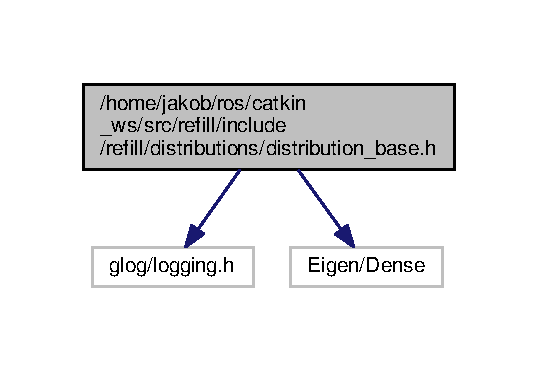
\includegraphics[width=258pt]{distribution__base_8h__incl}
\end{center}
\end{figure}
This graph shows which files directly or indirectly include this file\+:\nopagebreak
\begin{figure}[H]
\begin{center}
\leavevmode
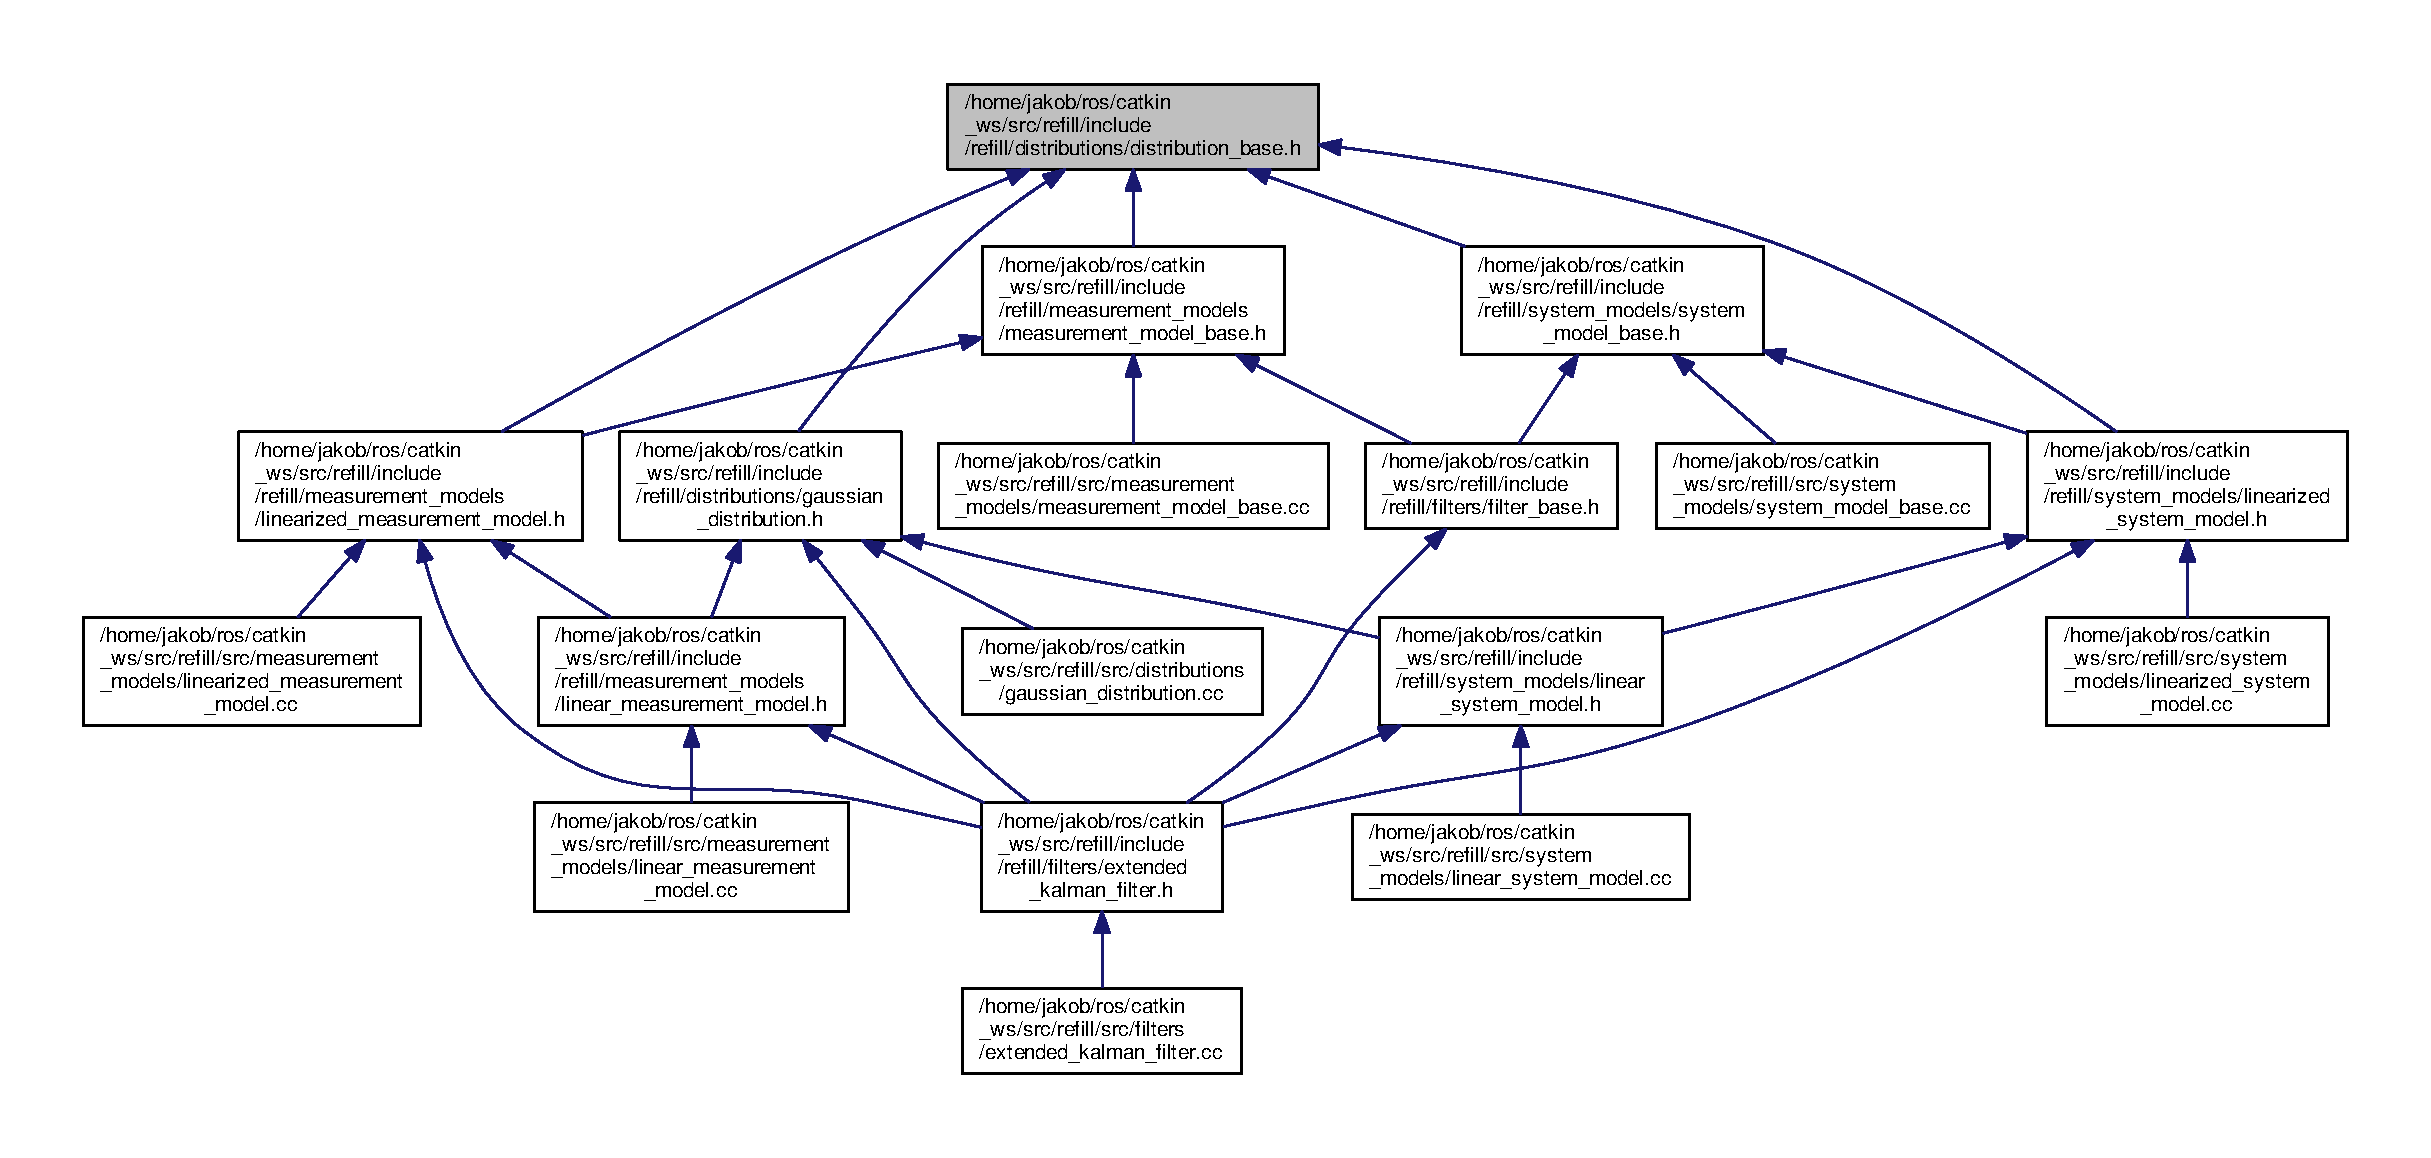
\includegraphics[width=350pt]{distribution__base_8h__dep__incl}
\end{center}
\end{figure}
\subsection*{Classes}
\begin{DoxyCompactItemize}
\item 
class \hyperlink{classrefill_1_1DistributionInterface}{refill\+::\+Distribution\+Interface}
\begin{DoxyCompactList}\small\item\em Interface for distributions. \end{DoxyCompactList}\item 
class \hyperlink{classrefill_1_1DistributionBase}{refill\+::\+Distribution\+Base$<$ D\+E\+R\+I\+V\+E\+D $>$}
\begin{DoxyCompactList}\small\item\em Class that implements the C\+R\+TP. \end{DoxyCompactList}\end{DoxyCompactItemize}
\subsection*{Namespaces}
\begin{DoxyCompactItemize}
\item 
 \hyperlink{namespacerefill}{refill}
\end{DoxyCompactItemize}

\hypertarget{gaussian__distribution_8h}{}\section{/home/jakob/ros/catkin\+\_\+ws/src/refill/include/refill/distributions/gaussian\+\_\+distribution.h File Reference}
\label{gaussian__distribution_8h}\index{/home/jakob/ros/catkin\+\_\+ws/src/refill/include/refill/distributions/gaussian\+\_\+distribution.\+h@{/home/jakob/ros/catkin\+\_\+ws/src/refill/include/refill/distributions/gaussian\+\_\+distribution.\+h}}
{\ttfamily \#include $<$glog/logging.\+h$>$}\\*
{\ttfamily \#include \char`\"{}refill/distributions/distribution\+\_\+base.\+h\char`\"{}}\\*
Include dependency graph for gaussian\+\_\+distribution.\+h\+:\nopagebreak
\begin{figure}[H]
\begin{center}
\leavevmode
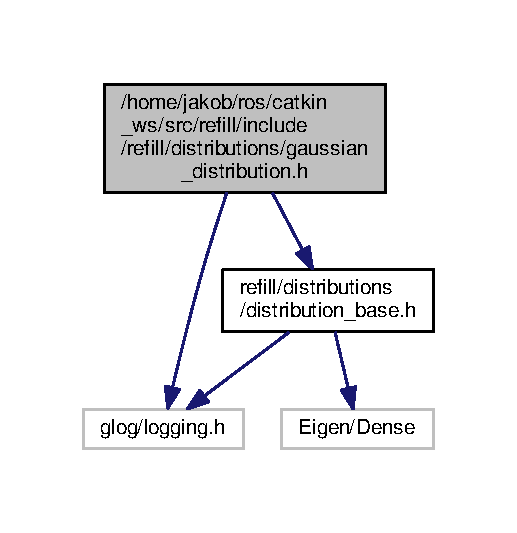
\includegraphics[width=248pt]{gaussian__distribution_8h__incl}
\end{center}
\end{figure}
This graph shows which files directly or indirectly include this file\+:\nopagebreak
\begin{figure}[H]
\begin{center}
\leavevmode
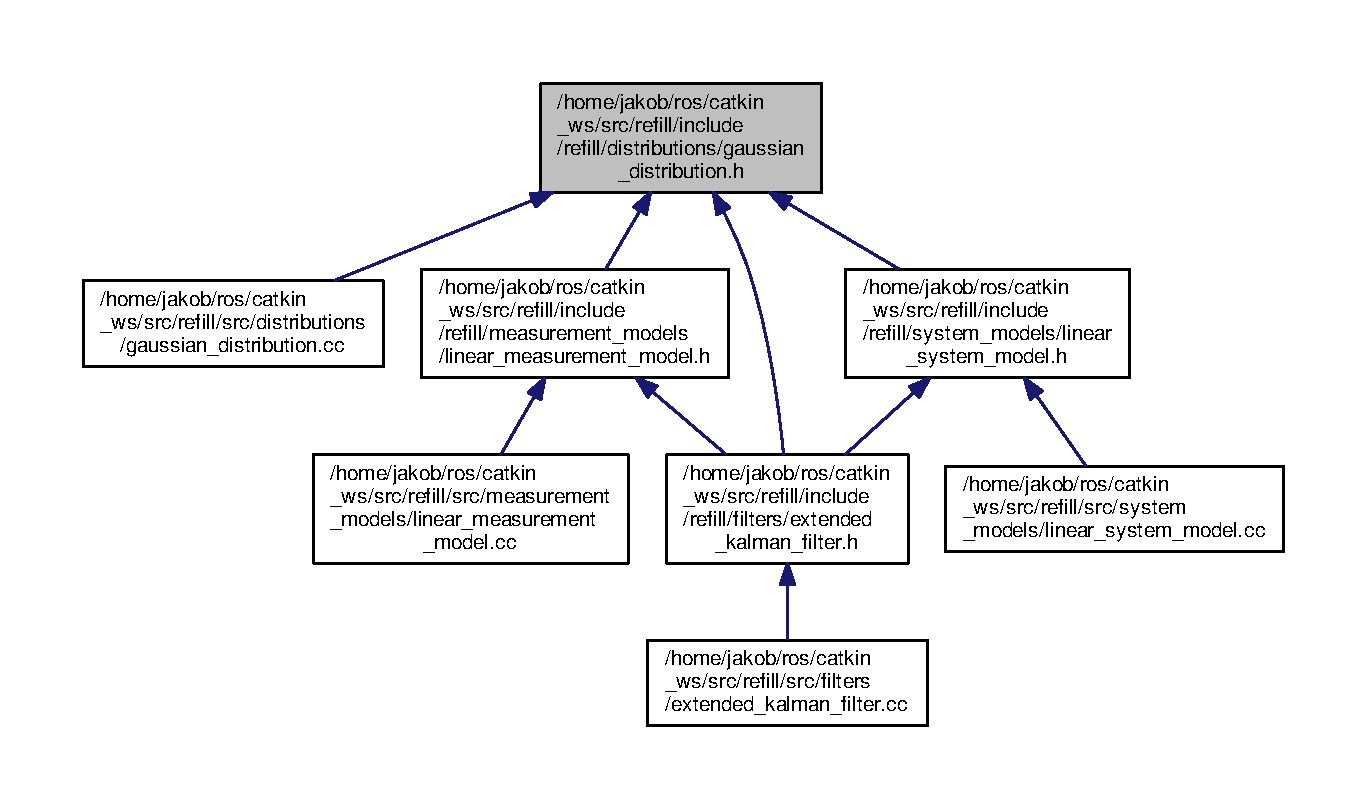
\includegraphics[width=350pt]{gaussian__distribution_8h__dep__incl}
\end{center}
\end{figure}
\subsection*{Classes}
\begin{DoxyCompactItemize}
\item 
class \hyperlink{classrefill_1_1GaussianDistribution}{refill\+::\+Gaussian\+Distribution}
\begin{DoxyCompactList}\small\item\em Class that implements a multivariate Gaussian distribution. \end{DoxyCompactList}\end{DoxyCompactItemize}
\subsection*{Namespaces}
\begin{DoxyCompactItemize}
\item 
 \hyperlink{namespacerefill}{refill}
\end{DoxyCompactItemize}

\hypertarget{extended__kalman__filter_8h}{}\section{/home/jakob/ros/catkin\+\_\+ws/src/refill/include/refill/filters/extended\+\_\+kalman\+\_\+filter.h File Reference}
\label{extended__kalman__filter_8h}\index{/home/jakob/ros/catkin\+\_\+ws/src/refill/include/refill/filters/extended\+\_\+kalman\+\_\+filter.\+h@{/home/jakob/ros/catkin\+\_\+ws/src/refill/include/refill/filters/extended\+\_\+kalman\+\_\+filter.\+h}}
{\ttfamily \#include $<$memory$>$}\\*
{\ttfamily \#include \char`\"{}refill/distributions/gaussian\+\_\+distribution.\+h\char`\"{}}\\*
{\ttfamily \#include \char`\"{}refill/filters/filter\+\_\+base.\+h\char`\"{}}\\*
{\ttfamily \#include \char`\"{}refill/measurement\+\_\+models/linear\+\_\+measurement\+\_\+model.\+h\char`\"{}}\\*
{\ttfamily \#include \char`\"{}refill/measurement\+\_\+models/linearized\+\_\+measurement\+\_\+model.\+h\char`\"{}}\\*
{\ttfamily \#include \char`\"{}refill/system\+\_\+models/linear\+\_\+system\+\_\+model.\+h\char`\"{}}\\*
{\ttfamily \#include \char`\"{}refill/system\+\_\+models/linearized\+\_\+system\+\_\+model.\+h\char`\"{}}\\*
Include dependency graph for extended\+\_\+kalman\+\_\+filter.\+h\+:\nopagebreak
\begin{figure}[H]
\begin{center}
\leavevmode
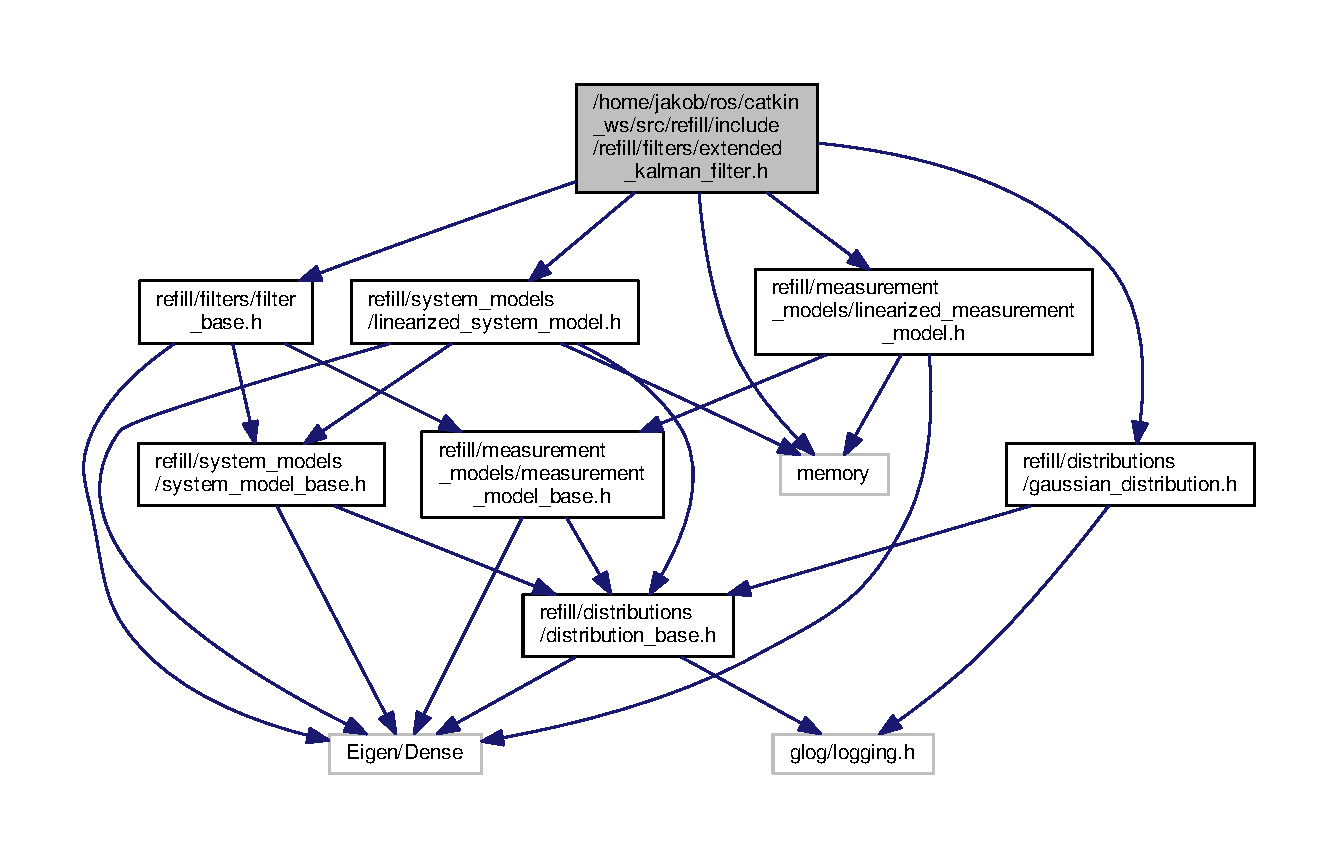
\includegraphics[width=350pt]{extended__kalman__filter_8h__incl}
\end{center}
\end{figure}
This graph shows which files directly or indirectly include this file\+:\nopagebreak
\begin{figure}[H]
\begin{center}
\leavevmode
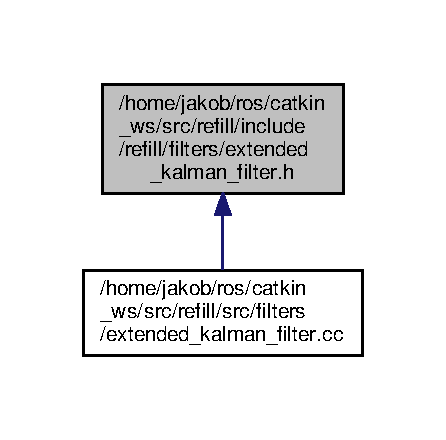
\includegraphics[width=214pt]{extended__kalman__filter_8h__dep__incl}
\end{center}
\end{figure}
\subsection*{Classes}
\begin{DoxyCompactItemize}
\item 
class \hyperlink{classrefill_1_1ExtendedKalmanFilter}{refill\+::\+Extended\+Kalman\+Filter}
\end{DoxyCompactItemize}
\subsection*{Namespaces}
\begin{DoxyCompactItemize}
\item 
 \hyperlink{namespacerefill}{refill}
\end{DoxyCompactItemize}

\hypertarget{filter__base_8h}{}\section{/home/jakob/ros/catkin\+\_\+ws/src/refill/include/refill/filters/filter\+\_\+base.h File Reference}
\label{filter__base_8h}\index{/home/jakob/ros/catkin\+\_\+ws/src/refill/include/refill/filters/filter\+\_\+base.\+h@{/home/jakob/ros/catkin\+\_\+ws/src/refill/include/refill/filters/filter\+\_\+base.\+h}}
{\ttfamily \#include $<$Eigen/\+Dense$>$}\\*
{\ttfamily \#include \char`\"{}refill/measurement\+\_\+models/measurement\+\_\+model\+\_\+base.\+h\char`\"{}}\\*
{\ttfamily \#include \char`\"{}refill/system\+\_\+models/system\+\_\+model\+\_\+base.\+h\char`\"{}}\\*
Include dependency graph for filter\+\_\+base.\+h\+:\nopagebreak
\begin{figure}[H]
\begin{center}
\leavevmode
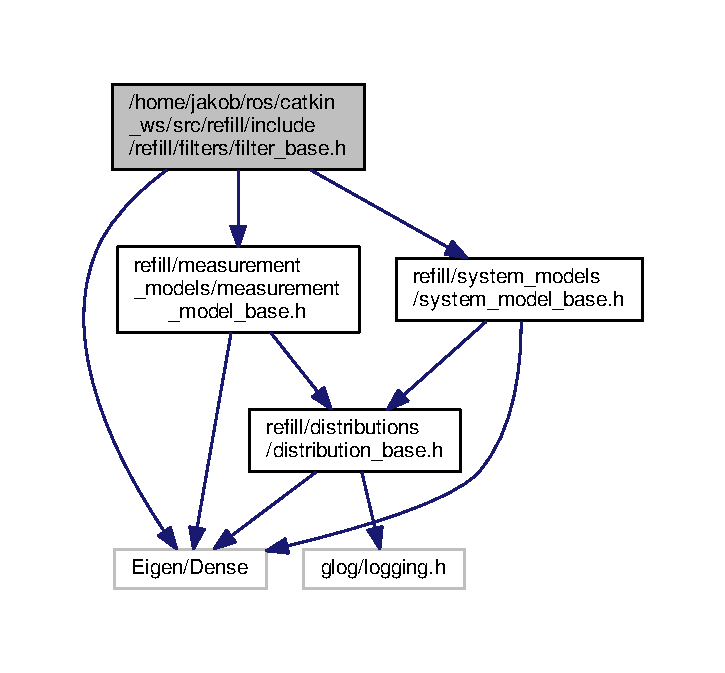
\includegraphics[width=348pt]{filter__base_8h__incl}
\end{center}
\end{figure}
This graph shows which files directly or indirectly include this file\+:\nopagebreak
\begin{figure}[H]
\begin{center}
\leavevmode
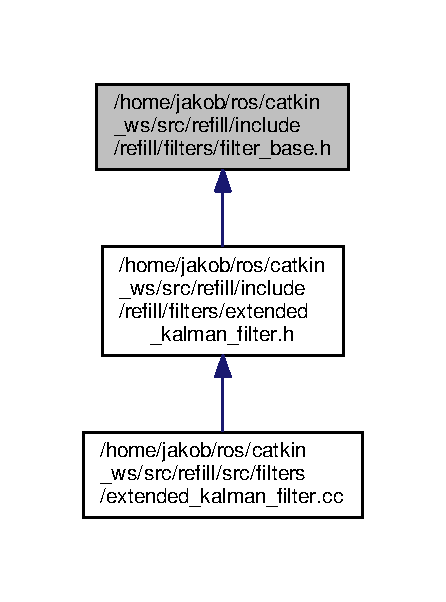
\includegraphics[width=214pt]{filter__base_8h__dep__incl}
\end{center}
\end{figure}
\subsection*{Classes}
\begin{DoxyCompactItemize}
\item 
class \hyperlink{classrefill_1_1FilterBase}{refill\+::\+Filter\+Base$<$ S\+Y\+S\+T\+E\+M\+\_\+\+M\+O\+D\+E\+L\+\_\+\+T\+Y\+P\+E, M\+E\+A\+S\+U\+R\+E\+M\+E\+N\+T\+\_\+\+M\+O\+D\+E\+L\+\_\+\+T\+Y\+P\+E $>$}
\end{DoxyCompactItemize}
\subsection*{Namespaces}
\begin{DoxyCompactItemize}
\item 
 \hyperlink{namespacerefill}{refill}
\end{DoxyCompactItemize}

\hypertarget{linear__measurement__model_8h}{}\section{/home/jakob/ros/catkin\+\_\+ws/src/refill/include/refill/measurement\+\_\+models/linear\+\_\+measurement\+\_\+model.h File Reference}
\label{linear__measurement__model_8h}\index{/home/jakob/ros/catkin\+\_\+ws/src/refill/include/refill/measurement\+\_\+models/linear\+\_\+measurement\+\_\+model.\+h@{/home/jakob/ros/catkin\+\_\+ws/src/refill/include/refill/measurement\+\_\+models/linear\+\_\+measurement\+\_\+model.\+h}}
{\ttfamily \#include $<$glog/logging.\+h$>$}\\*
{\ttfamily \#include $<$Eigen/\+Dense$>$}\\*
{\ttfamily \#include \char`\"{}refill/distributions/gaussian\+\_\+distribution.\+h\char`\"{}}\\*
{\ttfamily \#include \char`\"{}refill/measurement\+\_\+models/linearized\+\_\+measurement\+\_\+model.\+h\char`\"{}}\\*
Include dependency graph for linear\+\_\+measurement\+\_\+model.\+h\+:\nopagebreak
\begin{figure}[H]
\begin{center}
\leavevmode
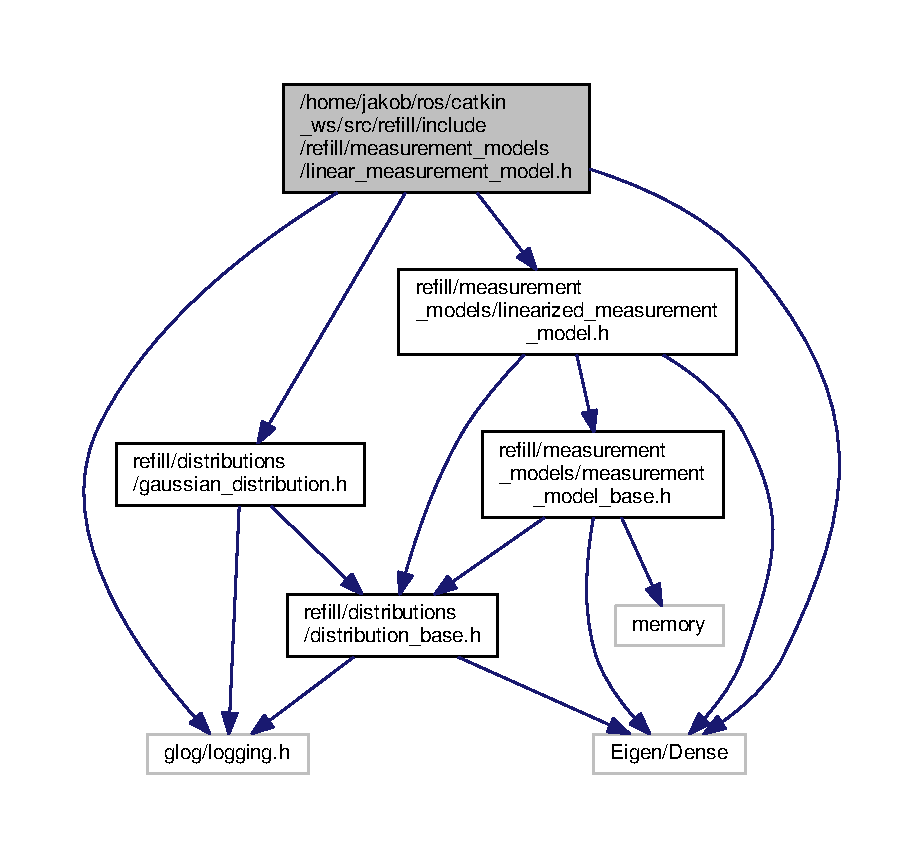
\includegraphics[width=350pt]{linear__measurement__model_8h__incl}
\end{center}
\end{figure}
This graph shows which files directly or indirectly include this file\+:\nopagebreak
\begin{figure}[H]
\begin{center}
\leavevmode
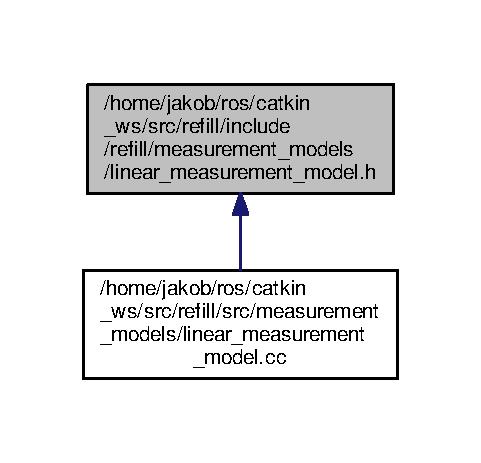
\includegraphics[width=350pt]{linear__measurement__model_8h__dep__incl}
\end{center}
\end{figure}
\subsection*{Classes}
\begin{DoxyCompactItemize}
\item 
class \hyperlink{classrefill_1_1LinearMeasurementModel}{refill\+::\+Linear\+Measurement\+Model}
\end{DoxyCompactItemize}
\subsection*{Namespaces}
\begin{DoxyCompactItemize}
\item 
 \hyperlink{namespacerefill}{refill}
\end{DoxyCompactItemize}

\hypertarget{linearized__measurement__model_8h}{}\section{/home/jakob/ros/catkin\+\_\+ws/src/refill/include/refill/measurement\+\_\+models/linearized\+\_\+measurement\+\_\+model.h File Reference}
\label{linearized__measurement__model_8h}\index{/home/jakob/ros/catkin\+\_\+ws/src/refill/include/refill/measurement\+\_\+models/linearized\+\_\+measurement\+\_\+model.\+h@{/home/jakob/ros/catkin\+\_\+ws/src/refill/include/refill/measurement\+\_\+models/linearized\+\_\+measurement\+\_\+model.\+h}}
{\ttfamily \#include $<$Eigen/\+Dense$>$}\\*
{\ttfamily \#include $<$memory$>$}\\*
{\ttfamily \#include \char`\"{}refill/measurement\+\_\+models/measurement\+\_\+model\+\_\+base.\+h\char`\"{}}\\*
Include dependency graph for linearized\+\_\+measurement\+\_\+model.\+h\+:\nopagebreak
\begin{figure}[H]
\begin{center}
\leavevmode
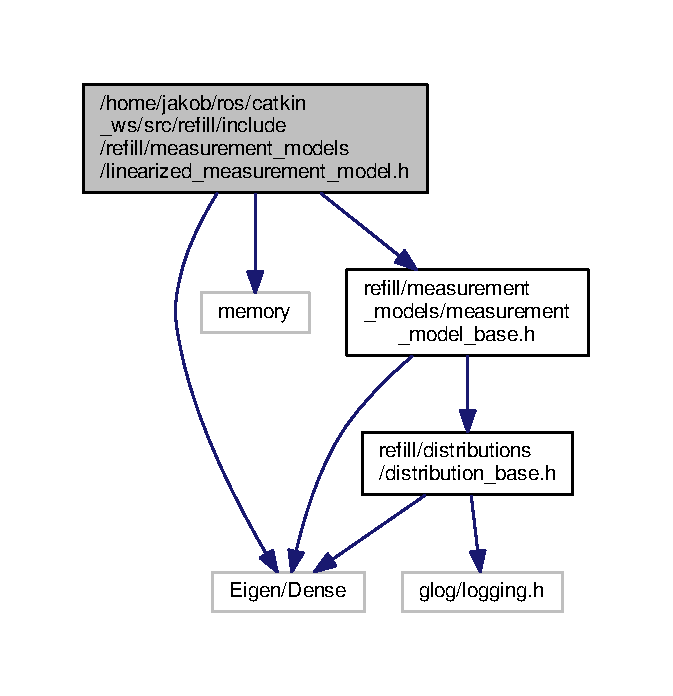
\includegraphics[width=323pt]{linearized__measurement__model_8h__incl}
\end{center}
\end{figure}
This graph shows which files directly or indirectly include this file\+:\nopagebreak
\begin{figure}[H]
\begin{center}
\leavevmode
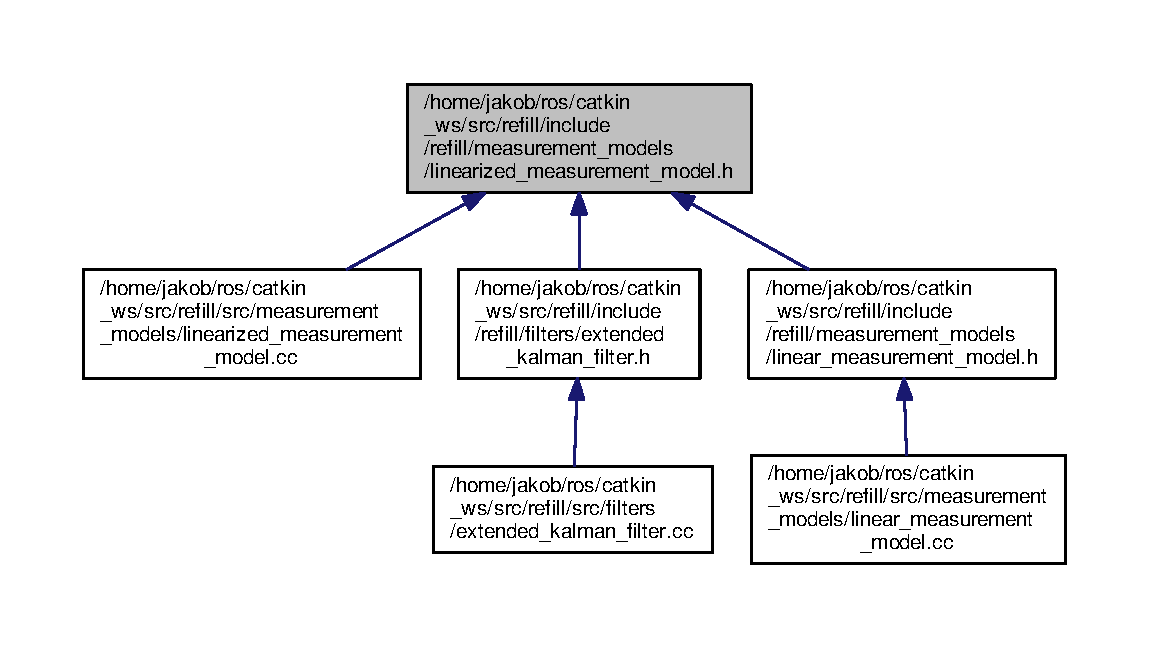
\includegraphics[width=350pt]{linearized__measurement__model_8h__dep__incl}
\end{center}
\end{figure}
\subsection*{Classes}
\begin{DoxyCompactItemize}
\item 
class \hyperlink{classrefill_1_1LinearizedMeasurementModel}{refill\+::\+Linearized\+Measurement\+Model}
\end{DoxyCompactItemize}
\subsection*{Namespaces}
\begin{DoxyCompactItemize}
\item 
 \hyperlink{namespacerefill}{refill}
\end{DoxyCompactItemize}

\hypertarget{measurement__model__base_8h}{}\section{/home/jakob/ros/catkin\+\_\+ws/src/refill/include/refill/measurement\+\_\+models/measurement\+\_\+model\+\_\+base.h File Reference}
\label{measurement__model__base_8h}\index{/home/jakob/ros/catkin\+\_\+ws/src/refill/include/refill/measurement\+\_\+models/measurement\+\_\+model\+\_\+base.\+h@{/home/jakob/ros/catkin\+\_\+ws/src/refill/include/refill/measurement\+\_\+models/measurement\+\_\+model\+\_\+base.\+h}}
{\ttfamily \#include $<$Eigen/\+Dense$>$}\\*
{\ttfamily \#include \char`\"{}refill/distributions/distribution\+\_\+base.\+h\char`\"{}}\\*
Include dependency graph for measurement\+\_\+model\+\_\+base.\+h\+:\nopagebreak
\begin{figure}[H]
\begin{center}
\leavevmode
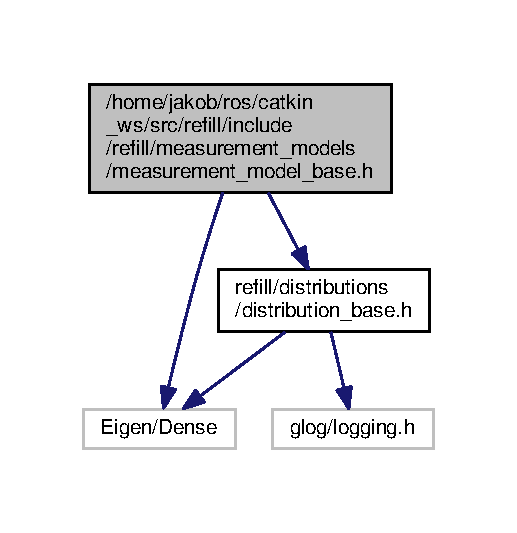
\includegraphics[width=248pt]{measurement__model__base_8h__incl}
\end{center}
\end{figure}
This graph shows which files directly or indirectly include this file\+:\nopagebreak
\begin{figure}[H]
\begin{center}
\leavevmode
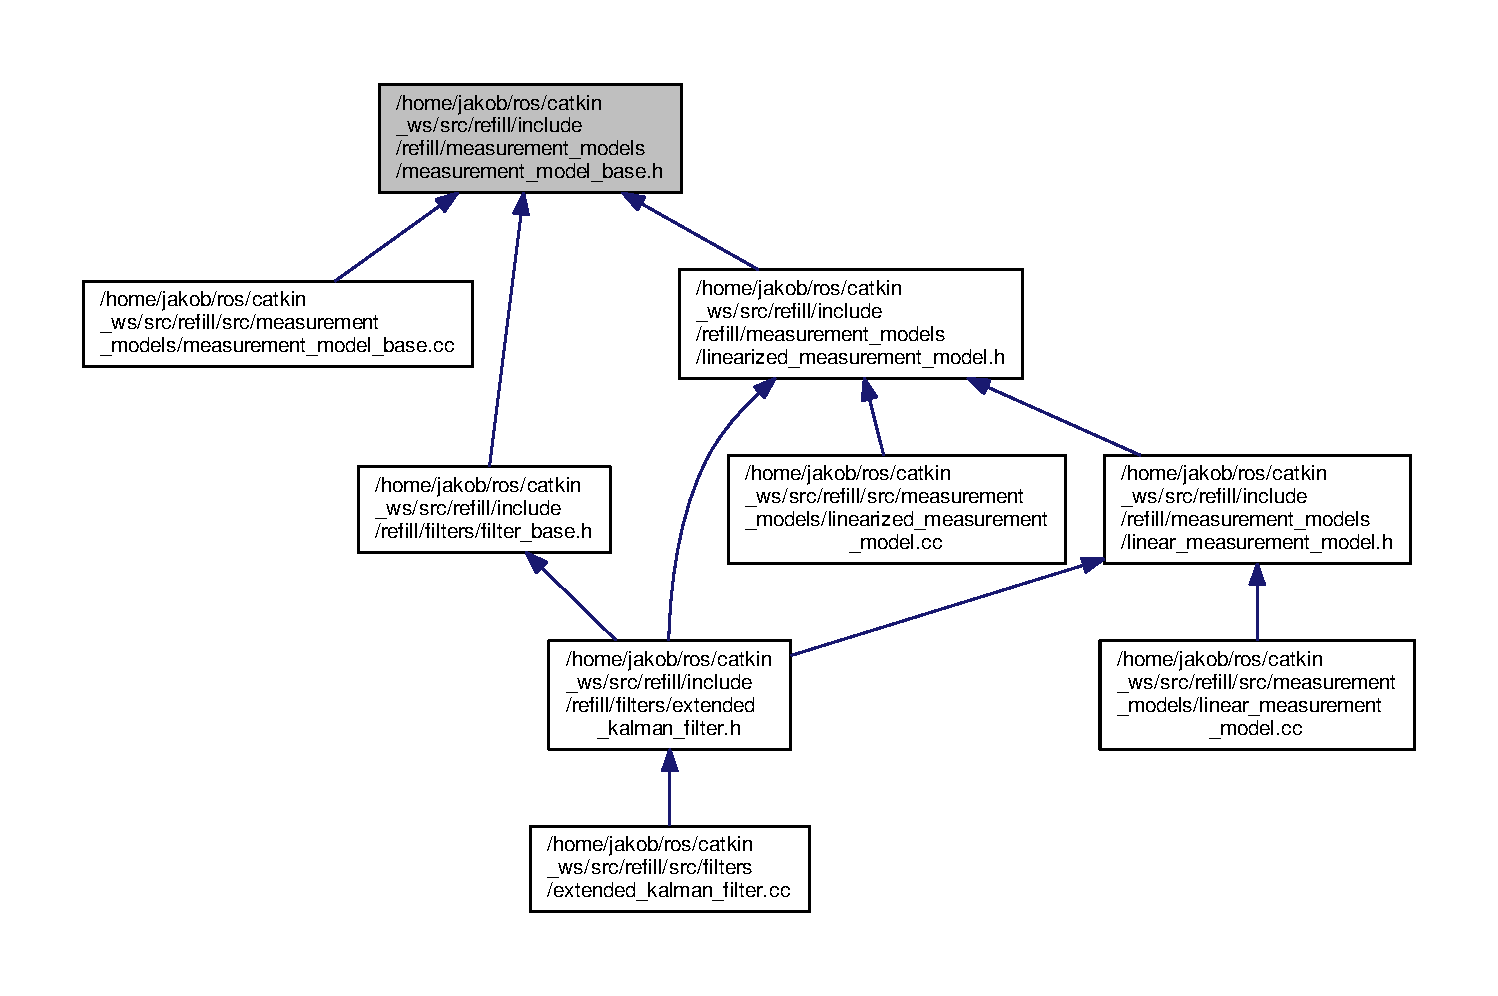
\includegraphics[width=350pt]{measurement__model__base_8h__dep__incl}
\end{center}
\end{figure}
\subsection*{Classes}
\begin{DoxyCompactItemize}
\item 
class \hyperlink{classrefill_1_1MeasurementModelBase}{refill\+::\+Measurement\+Model\+Base}
\end{DoxyCompactItemize}
\subsection*{Namespaces}
\begin{DoxyCompactItemize}
\item 
 \hyperlink{namespacerefill}{refill}
\end{DoxyCompactItemize}

\hypertarget{linear__system__model_8h}{}\section{/home/jakob/ros/catkin\+\_\+ws/src/refill/include/refill/system\+\_\+models/linear\+\_\+system\+\_\+model.h File Reference}
\label{linear__system__model_8h}\index{/home/jakob/ros/catkin\+\_\+ws/src/refill/include/refill/system\+\_\+models/linear\+\_\+system\+\_\+model.\+h@{/home/jakob/ros/catkin\+\_\+ws/src/refill/include/refill/system\+\_\+models/linear\+\_\+system\+\_\+model.\+h}}
{\ttfamily \#include $<$Eigen/\+Dense$>$}\\*
{\ttfamily \#include $<$glog/logging.\+h$>$}\\*
{\ttfamily \#include \char`\"{}refill/system\+\_\+models/linearized\+\_\+system\+\_\+model.\+h\char`\"{}}\\*
{\ttfamily \#include \char`\"{}refill/distributions/gaussian\+\_\+distribution.\+h\char`\"{}}\\*
Include dependency graph for linear\+\_\+system\+\_\+model.\+h\+:\nopagebreak
\begin{figure}[H]
\begin{center}
\leavevmode
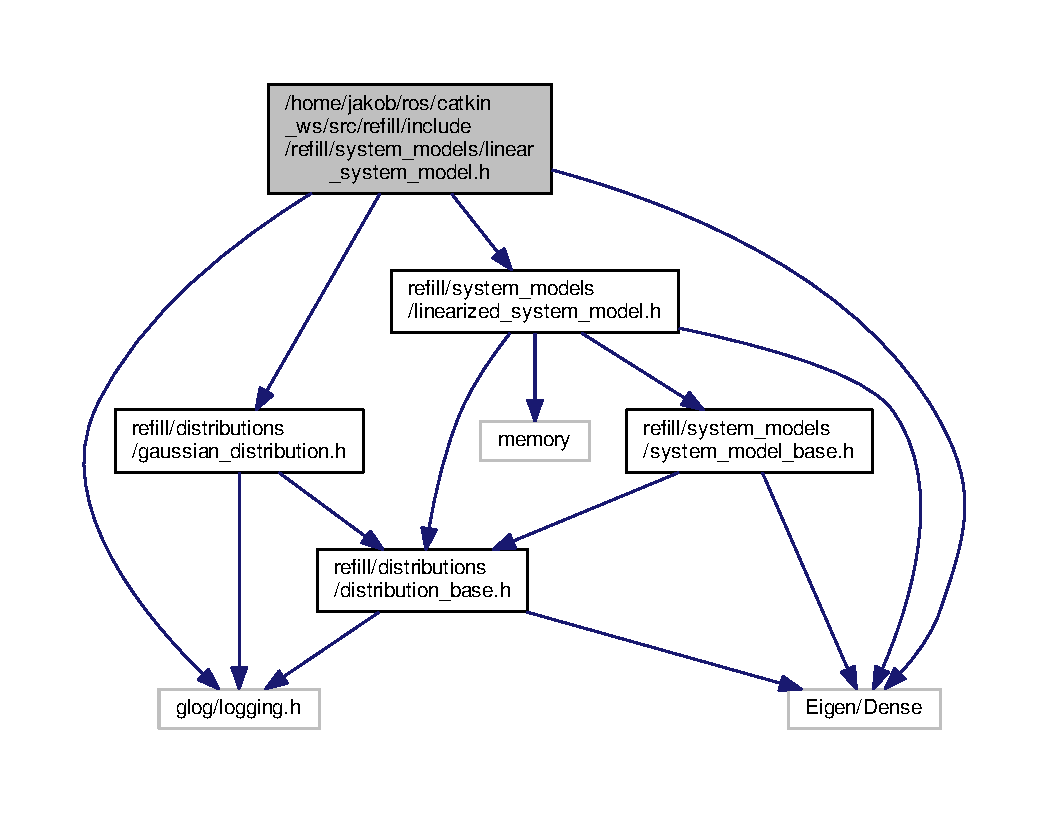
\includegraphics[width=350pt]{linear__system__model_8h__incl}
\end{center}
\end{figure}
This graph shows which files directly or indirectly include this file\+:\nopagebreak
\begin{figure}[H]
\begin{center}
\leavevmode
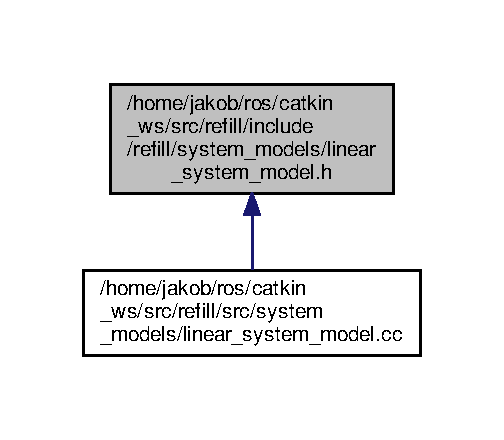
\includegraphics[width=242pt]{linear__system__model_8h__dep__incl}
\end{center}
\end{figure}
\subsection*{Classes}
\begin{DoxyCompactItemize}
\item 
class \hyperlink{classrefill_1_1LinearSystemModel}{refill\+::\+Linear\+System\+Model}
\end{DoxyCompactItemize}
\subsection*{Namespaces}
\begin{DoxyCompactItemize}
\item 
 \hyperlink{namespacerefill}{refill}
\end{DoxyCompactItemize}

\hypertarget{linearized__system__model_8h}{}\section{/home/jakob/ros/catkin\+\_\+ws/src/refill/include/refill/system\+\_\+models/linearized\+\_\+system\+\_\+model.h File Reference}
\label{linearized__system__model_8h}\index{/home/jakob/ros/catkin\+\_\+ws/src/refill/include/refill/system\+\_\+models/linearized\+\_\+system\+\_\+model.\+h@{/home/jakob/ros/catkin\+\_\+ws/src/refill/include/refill/system\+\_\+models/linearized\+\_\+system\+\_\+model.\+h}}
{\ttfamily \#include $<$Eigen/\+Dense$>$}\\*
{\ttfamily \#include $<$memory$>$}\\*
{\ttfamily \#include \char`\"{}refill/distributions/distribution\+\_\+base.\+h\char`\"{}}\\*
{\ttfamily \#include \char`\"{}refill/system\+\_\+models/system\+\_\+model\+\_\+base.\+h\char`\"{}}\\*
Include dependency graph for linearized\+\_\+system\+\_\+model.\+h\+:\nopagebreak
\begin{figure}[H]
\begin{center}
\leavevmode
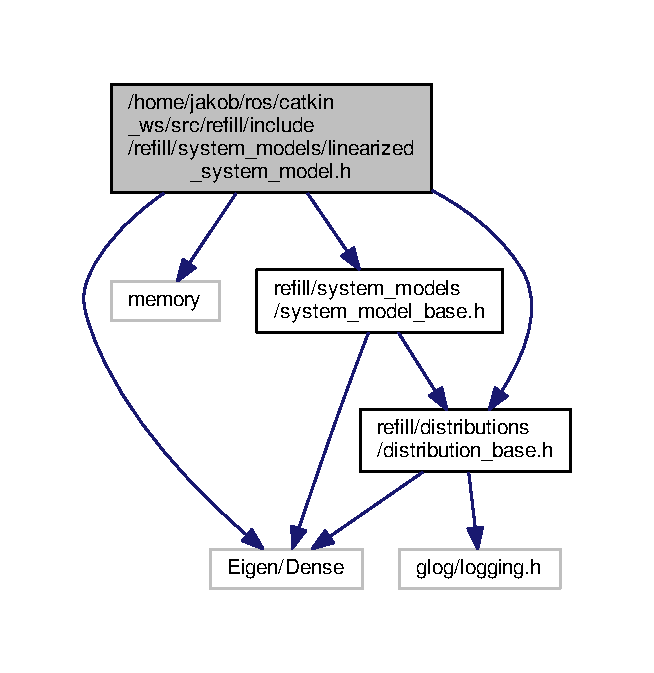
\includegraphics[width=314pt]{linearized__system__model_8h__incl}
\end{center}
\end{figure}
This graph shows which files directly or indirectly include this file\+:\nopagebreak
\begin{figure}[H]
\begin{center}
\leavevmode
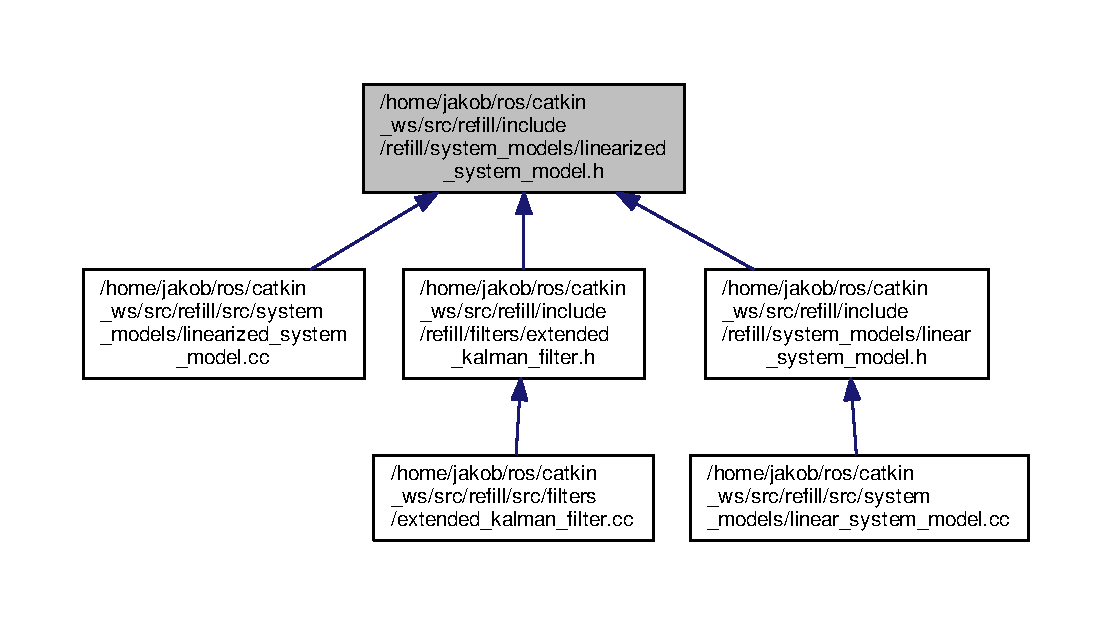
\includegraphics[width=350pt]{linearized__system__model_8h__dep__incl}
\end{center}
\end{figure}
\subsection*{Classes}
\begin{DoxyCompactItemize}
\item 
class \hyperlink{classrefill_1_1LinearizedSystemModel}{refill\+::\+Linearized\+System\+Model}
\end{DoxyCompactItemize}
\subsection*{Namespaces}
\begin{DoxyCompactItemize}
\item 
 \hyperlink{namespacerefill}{refill}
\end{DoxyCompactItemize}

\hypertarget{system__model__base_8h}{}\section{/home/jakob/ros/catkin\+\_\+ws/src/refill/include/refill/system\+\_\+models/system\+\_\+model\+\_\+base.h File Reference}
\label{system__model__base_8h}\index{/home/jakob/ros/catkin\+\_\+ws/src/refill/include/refill/system\+\_\+models/system\+\_\+model\+\_\+base.\+h@{/home/jakob/ros/catkin\+\_\+ws/src/refill/include/refill/system\+\_\+models/system\+\_\+model\+\_\+base.\+h}}
{\ttfamily \#include $<$Eigen/\+Dense$>$}\\*
{\ttfamily \#include \char`\"{}refill/distributions/distribution\+\_\+base.\+h\char`\"{}}\\*
Include dependency graph for system\+\_\+model\+\_\+base.\+h\+:\nopagebreak
\begin{figure}[H]
\begin{center}
\leavevmode
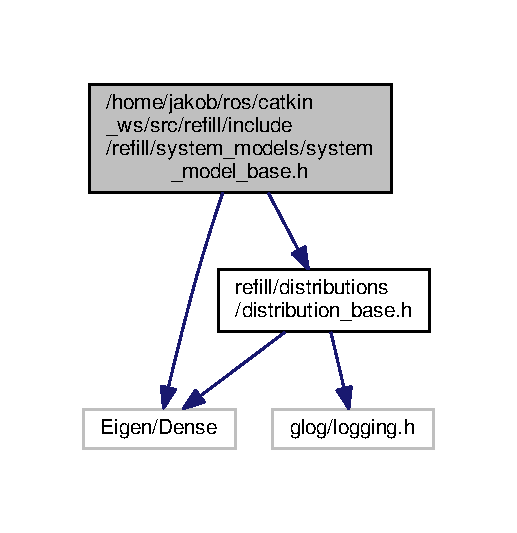
\includegraphics[width=248pt]{system__model__base_8h__incl}
\end{center}
\end{figure}
This graph shows which files directly or indirectly include this file\+:\nopagebreak
\begin{figure}[H]
\begin{center}
\leavevmode
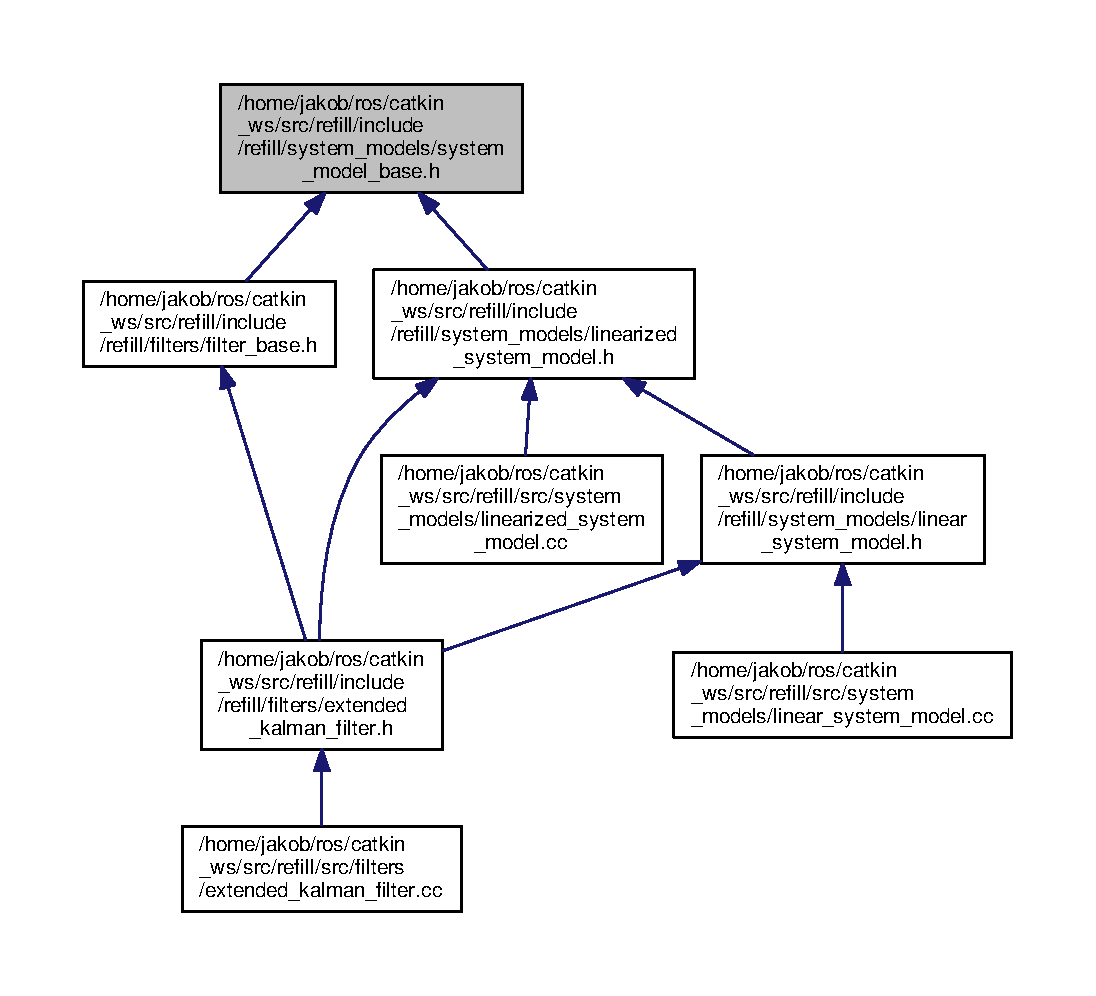
\includegraphics[width=350pt]{system__model__base_8h__dep__incl}
\end{center}
\end{figure}
\subsection*{Classes}
\begin{DoxyCompactItemize}
\item 
class \hyperlink{classrefill_1_1SystemModelBase}{refill\+::\+System\+Model\+Base}
\begin{DoxyCompactList}\small\item\em Interface for system models. \end{DoxyCompactList}\end{DoxyCompactItemize}
\subsection*{Namespaces}
\begin{DoxyCompactItemize}
\item 
 \hyperlink{namespacerefill}{refill}
\end{DoxyCompactItemize}

\hypertarget{gaussian__distribution_8cc}{}\section{/home/jakob/ros/catkin\+\_\+ws/src/refill/src/distributions/gaussian\+\_\+distribution.cc File Reference}
\label{gaussian__distribution_8cc}\index{/home/jakob/ros/catkin\+\_\+ws/src/refill/src/distributions/gaussian\+\_\+distribution.\+cc@{/home/jakob/ros/catkin\+\_\+ws/src/refill/src/distributions/gaussian\+\_\+distribution.\+cc}}
{\ttfamily \#include \char`\"{}refill/distributions/gaussian\+\_\+distribution.\+h\char`\"{}}\\*
Include dependency graph for gaussian\+\_\+distribution.\+cc\+:\nopagebreak
\begin{figure}[H]
\begin{center}
\leavevmode
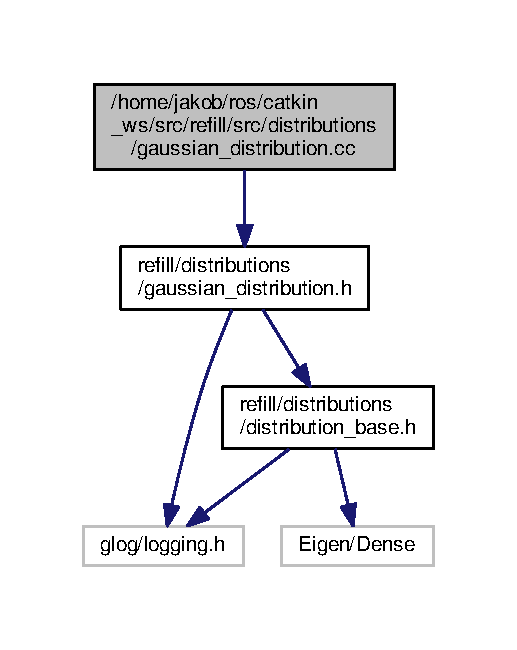
\includegraphics[width=248pt]{gaussian__distribution_8cc__incl}
\end{center}
\end{figure}
\subsection*{Namespaces}
\begin{DoxyCompactItemize}
\item 
 \hyperlink{namespacerefill}{refill}
\end{DoxyCompactItemize}

\hypertarget{extended__kalman__filter_8cc}{}\section{/home/jakob/ros/catkin\+\_\+ws/src/refill/src/filters/extended\+\_\+kalman\+\_\+filter.cc File Reference}
\label{extended__kalman__filter_8cc}\index{/home/jakob/ros/catkin\+\_\+ws/src/refill/src/filters/extended\+\_\+kalman\+\_\+filter.\+cc@{/home/jakob/ros/catkin\+\_\+ws/src/refill/src/filters/extended\+\_\+kalman\+\_\+filter.\+cc}}
{\ttfamily \#include \char`\"{}refill/filters/extended\+\_\+kalman\+\_\+filter.\+h\char`\"{}}\\*
Include dependency graph for extended\+\_\+kalman\+\_\+filter.\+cc\+:\nopagebreak
\begin{figure}[H]
\begin{center}
\leavevmode
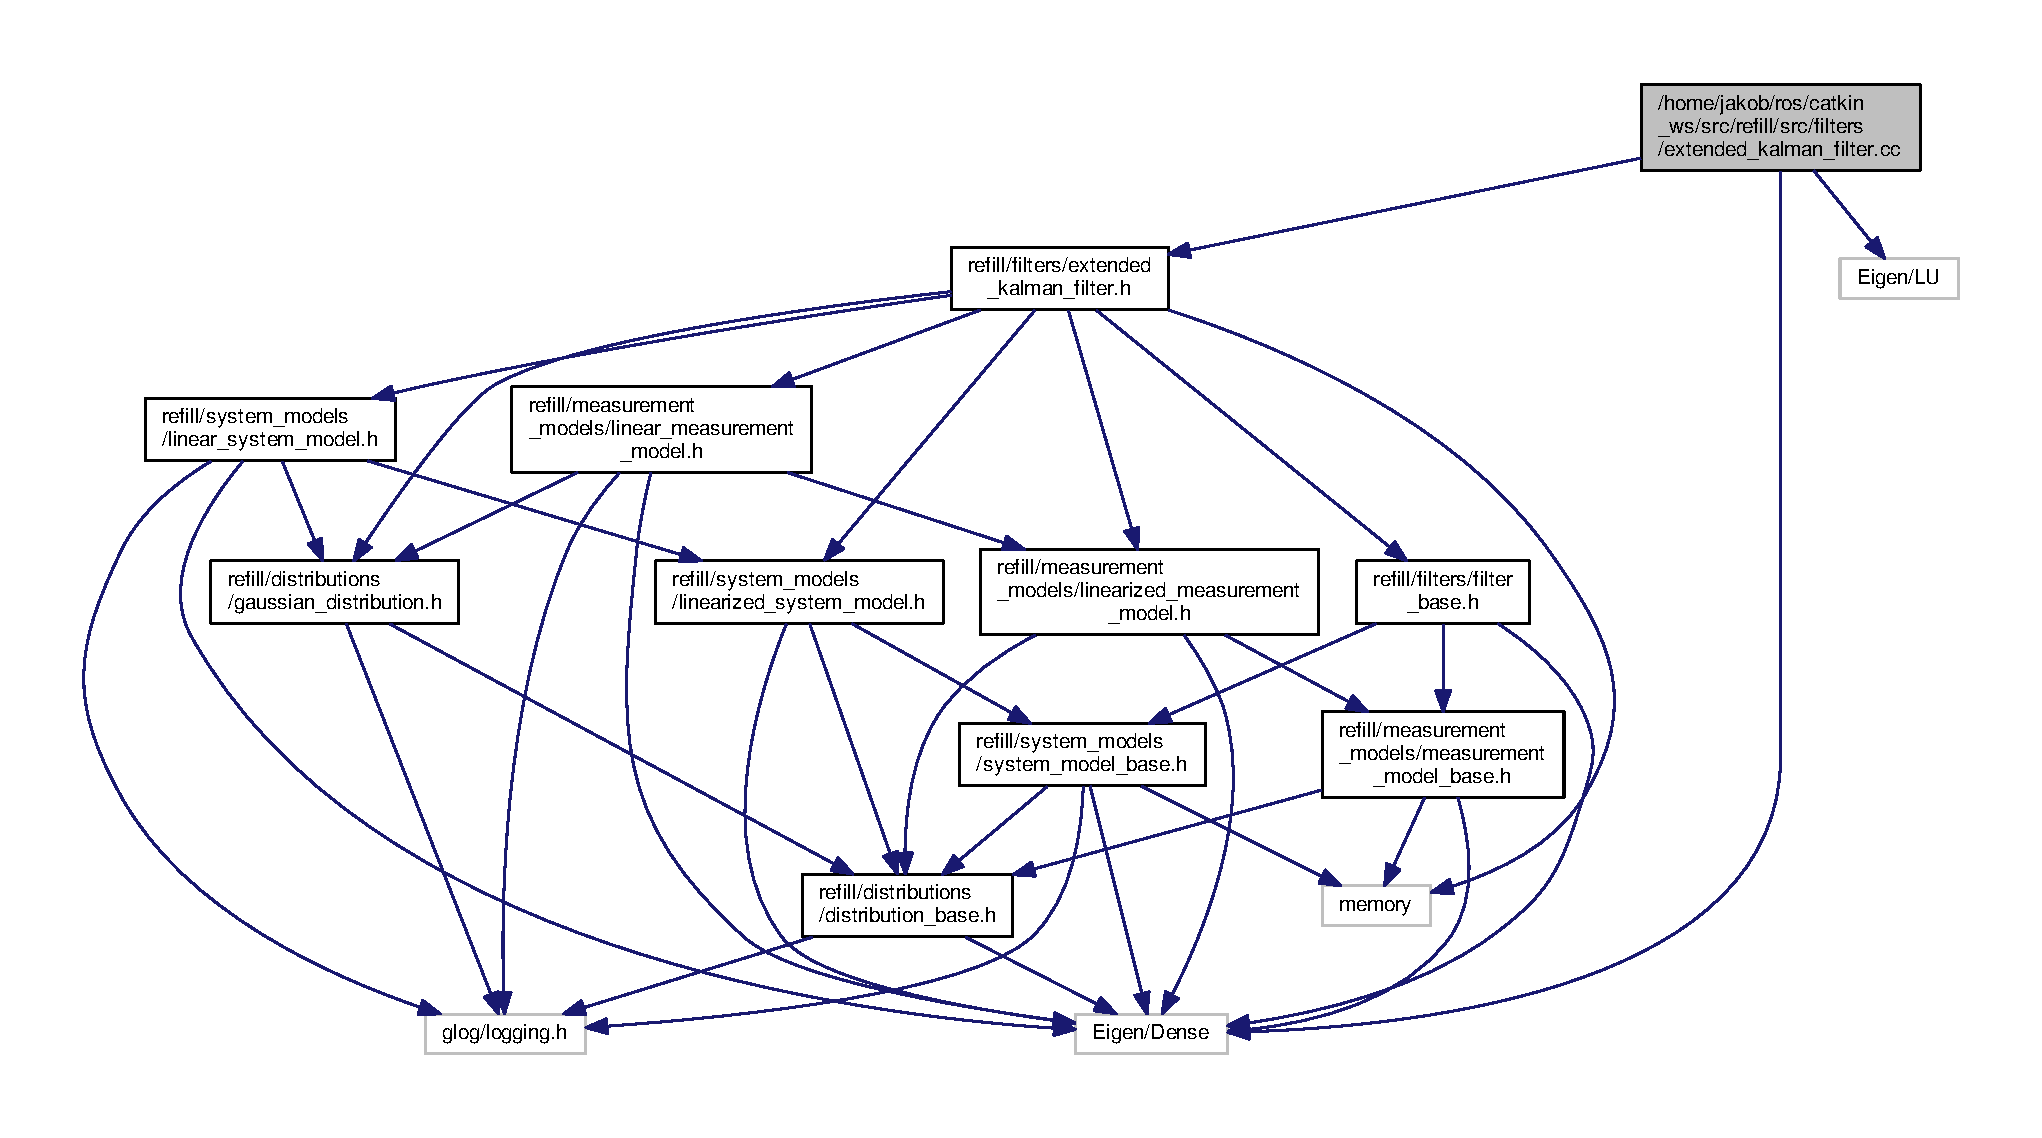
\includegraphics[width=350pt]{extended__kalman__filter_8cc__incl}
\end{center}
\end{figure}
\subsection*{Namespaces}
\begin{DoxyCompactItemize}
\item 
 \hyperlink{namespacerefill}{refill}
\end{DoxyCompactItemize}

\hypertarget{linear__measurement__model_8cc}{}\section{/home/jakob/ros/catkin\+\_\+ws/src/refill/src/measurement\+\_\+models/linear\+\_\+measurement\+\_\+model.cc File Reference}
\label{linear__measurement__model_8cc}\index{/home/jakob/ros/catkin\+\_\+ws/src/refill/src/measurement\+\_\+models/linear\+\_\+measurement\+\_\+model.\+cc@{/home/jakob/ros/catkin\+\_\+ws/src/refill/src/measurement\+\_\+models/linear\+\_\+measurement\+\_\+model.\+cc}}
{\ttfamily \#include \char`\"{}refill/measurement\+\_\+models/linear\+\_\+measurement\+\_\+model.\+h\char`\"{}}\\*
Include dependency graph for linear\+\_\+measurement\+\_\+model.\+cc\+:\nopagebreak
\begin{figure}[H]
\begin{center}
\leavevmode
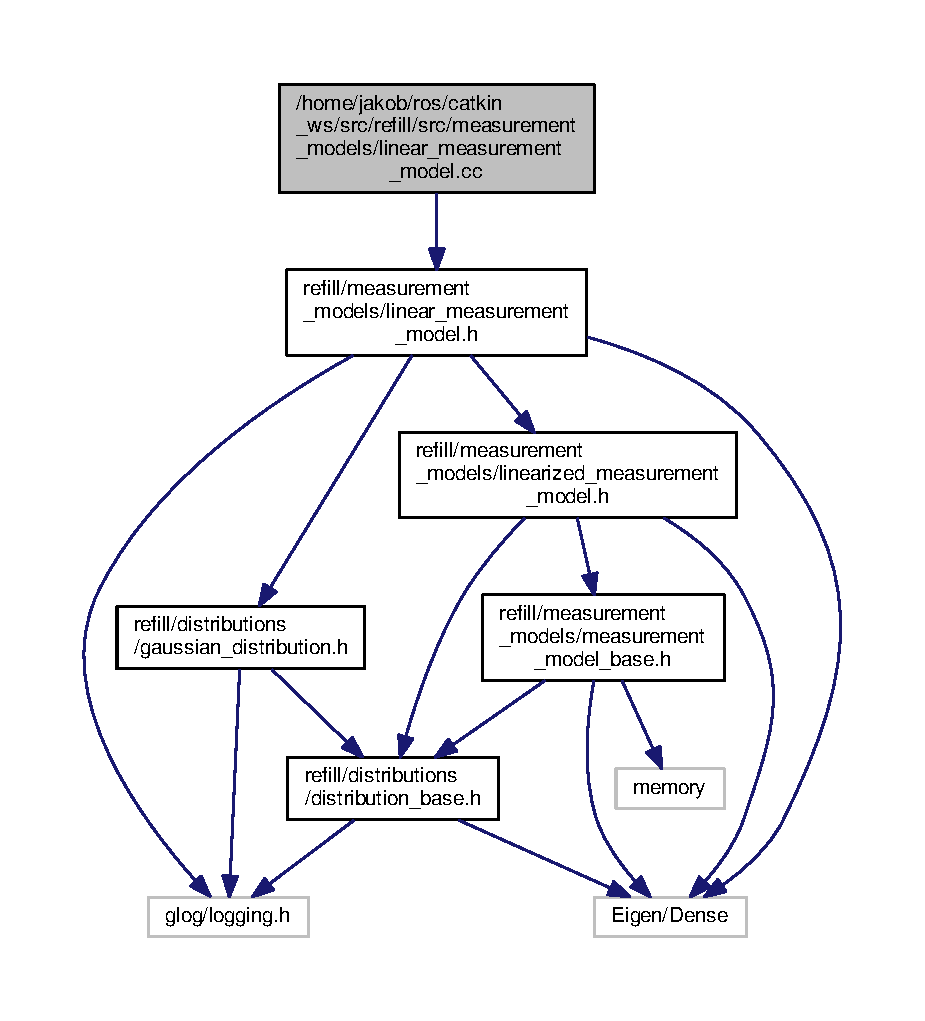
\includegraphics[width=350pt]{linear__measurement__model_8cc__incl}
\end{center}
\end{figure}
\subsection*{Namespaces}
\begin{DoxyCompactItemize}
\item 
 \hyperlink{namespacerefill}{refill}
\end{DoxyCompactItemize}

\hypertarget{linearized__measurement__model_8cc}{}\section{/home/jakob/ros/catkin\+\_\+ws/src/refill/src/measurement\+\_\+models/linearized\+\_\+measurement\+\_\+model.cc File Reference}
\label{linearized__measurement__model_8cc}\index{/home/jakob/ros/catkin\+\_\+ws/src/refill/src/measurement\+\_\+models/linearized\+\_\+measurement\+\_\+model.\+cc@{/home/jakob/ros/catkin\+\_\+ws/src/refill/src/measurement\+\_\+models/linearized\+\_\+measurement\+\_\+model.\+cc}}
{\ttfamily \#include \char`\"{}refill/measurement\+\_\+models/linearized\+\_\+measurement\+\_\+model.\+h\char`\"{}}\\*
Include dependency graph for linearized\+\_\+measurement\+\_\+model.\+cc\+:\nopagebreak
\begin{figure}[H]
\begin{center}
\leavevmode
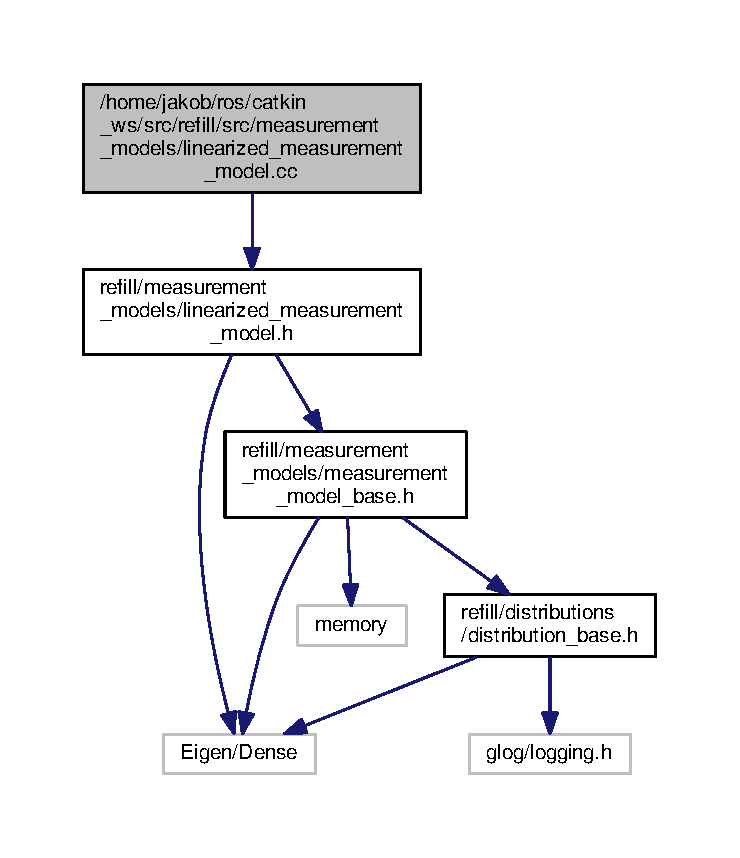
\includegraphics[width=350pt]{linearized__measurement__model_8cc__incl}
\end{center}
\end{figure}
\subsection*{Namespaces}
\begin{DoxyCompactItemize}
\item 
 \hyperlink{namespacerefill}{refill}
\end{DoxyCompactItemize}

\hypertarget{measurement__model__base_8cc}{}\section{/home/jakob/ros/catkin\+\_\+ws/src/refill/src/measurement\+\_\+models/measurement\+\_\+model\+\_\+base.cc File Reference}
\label{measurement__model__base_8cc}\index{/home/jakob/ros/catkin\+\_\+ws/src/refill/src/measurement\+\_\+models/measurement\+\_\+model\+\_\+base.\+cc@{/home/jakob/ros/catkin\+\_\+ws/src/refill/src/measurement\+\_\+models/measurement\+\_\+model\+\_\+base.\+cc}}
{\ttfamily \#include \char`\"{}refill/measurement\+\_\+models/measurement\+\_\+model\+\_\+base.\+h\char`\"{}}\\*
Include dependency graph for measurement\+\_\+model\+\_\+base.\+cc\+:\nopagebreak
\begin{figure}[H]
\begin{center}
\leavevmode
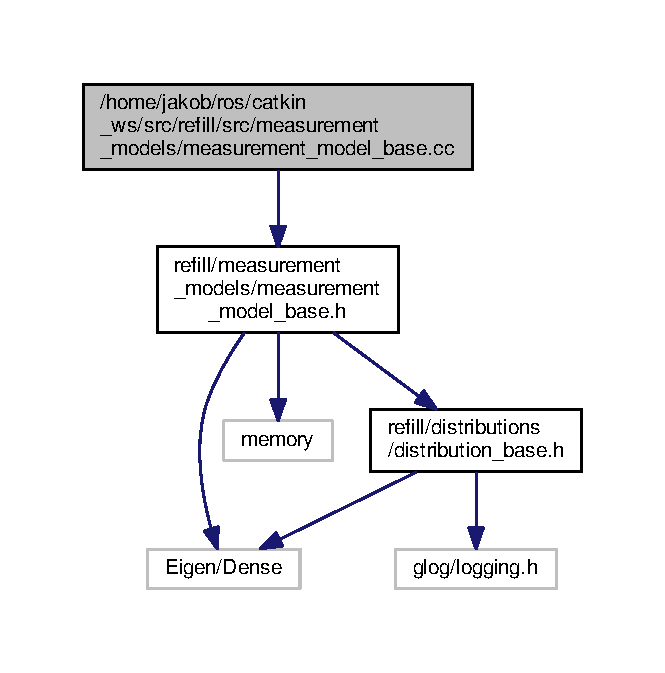
\includegraphics[width=319pt]{measurement__model__base_8cc__incl}
\end{center}
\end{figure}
\subsection*{Namespaces}
\begin{DoxyCompactItemize}
\item 
 \hyperlink{namespacerefill}{refill}
\end{DoxyCompactItemize}

\hypertarget{linear__system__model_8cc}{}\section{/home/jakob/ros/catkin\+\_\+ws/src/refill/src/system\+\_\+models/linear\+\_\+system\+\_\+model.cc File Reference}
\label{linear__system__model_8cc}\index{/home/jakob/ros/catkin\+\_\+ws/src/refill/src/system\+\_\+models/linear\+\_\+system\+\_\+model.\+cc@{/home/jakob/ros/catkin\+\_\+ws/src/refill/src/system\+\_\+models/linear\+\_\+system\+\_\+model.\+cc}}
{\ttfamily \#include \char`\"{}refill/system\+\_\+models/linear\+\_\+system\+\_\+model.\+h\char`\"{}}\\*
Include dependency graph for linear\+\_\+system\+\_\+model.\+cc\+:\nopagebreak
\begin{figure}[H]
\begin{center}
\leavevmode
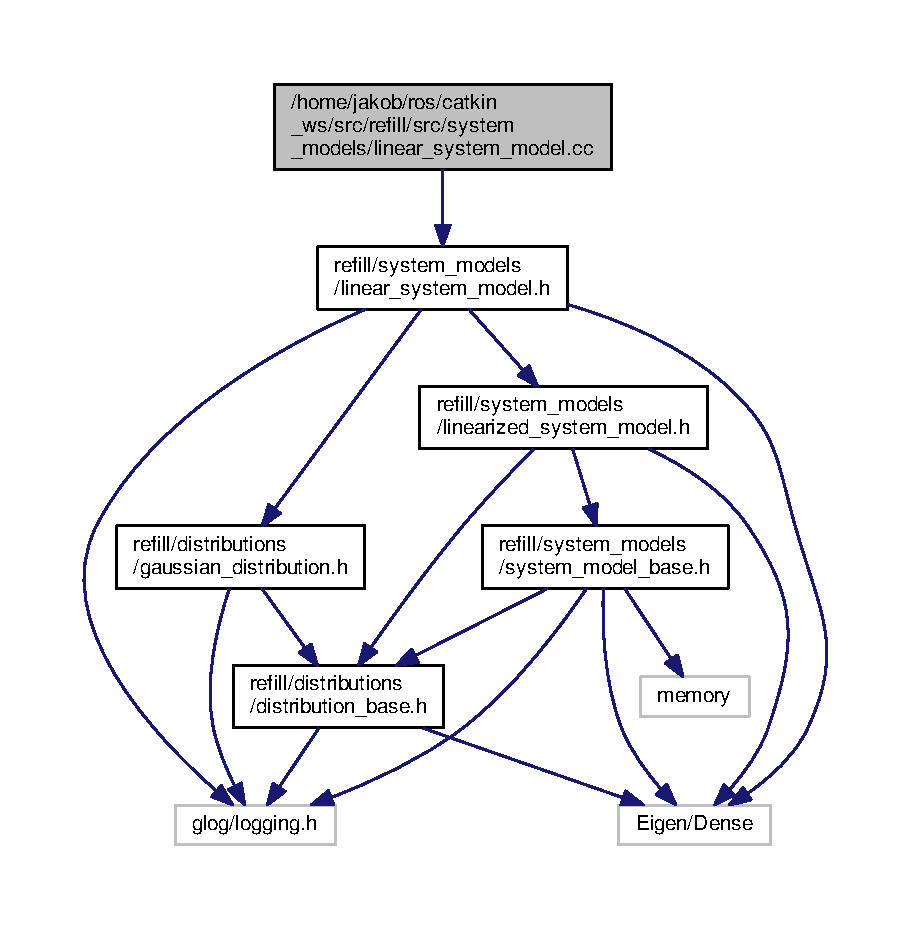
\includegraphics[width=350pt]{linear__system__model_8cc__incl}
\end{center}
\end{figure}
\subsection*{Namespaces}
\begin{DoxyCompactItemize}
\item 
 \hyperlink{namespacerefill}{refill}
\end{DoxyCompactItemize}

\hypertarget{linearized__system__model_8cc}{}\section{/home/jakob/ros/catkin\+\_\+ws/src/refill/src/system\+\_\+models/linearized\+\_\+system\+\_\+model.cc File Reference}
\label{linearized__system__model_8cc}\index{/home/jakob/ros/catkin\+\_\+ws/src/refill/src/system\+\_\+models/linearized\+\_\+system\+\_\+model.\+cc@{/home/jakob/ros/catkin\+\_\+ws/src/refill/src/system\+\_\+models/linearized\+\_\+system\+\_\+model.\+cc}}
{\ttfamily \#include \char`\"{}refill/system\+\_\+models/linearized\+\_\+system\+\_\+model.\+h\char`\"{}}\\*
Include dependency graph for linearized\+\_\+system\+\_\+model.\+cc\+:\nopagebreak
\begin{figure}[H]
\begin{center}
\leavevmode
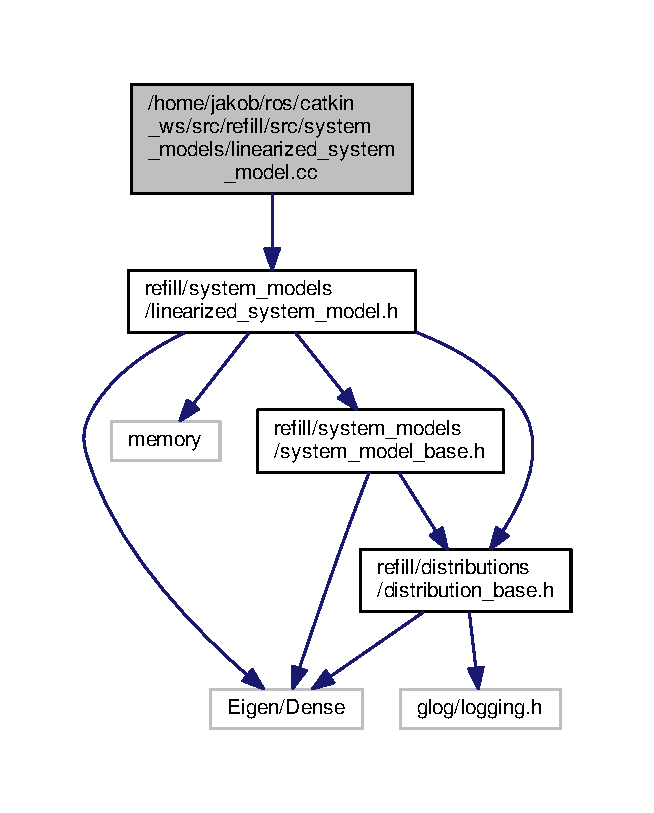
\includegraphics[width=314pt]{linearized__system__model_8cc__incl}
\end{center}
\end{figure}
\subsection*{Namespaces}
\begin{DoxyCompactItemize}
\item 
 \hyperlink{namespacerefill}{refill}
\end{DoxyCompactItemize}

\hypertarget{system__model__base_8cc}{}\section{/home/jakob/ros/catkin\+\_\+ws/src/refill/src/system\+\_\+models/system\+\_\+model\+\_\+base.cc File Reference}
\label{system__model__base_8cc}\index{/home/jakob/ros/catkin\+\_\+ws/src/refill/src/system\+\_\+models/system\+\_\+model\+\_\+base.\+cc@{/home/jakob/ros/catkin\+\_\+ws/src/refill/src/system\+\_\+models/system\+\_\+model\+\_\+base.\+cc}}
{\ttfamily \#include \char`\"{}refill/system\+\_\+models/system\+\_\+model\+\_\+base.\+h\char`\"{}}\\*
Include dependency graph for system\+\_\+model\+\_\+base.\+cc\+:\nopagebreak
\begin{figure}[H]
\begin{center}
\leavevmode
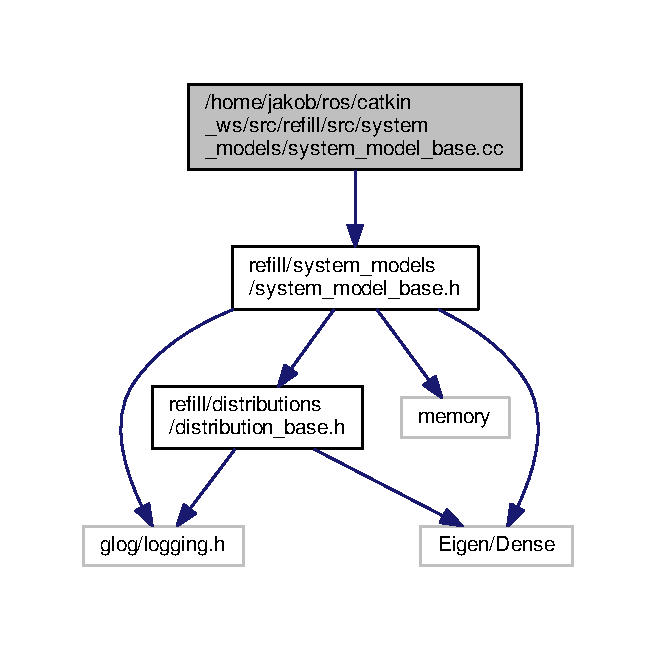
\includegraphics[width=315pt]{system__model__base_8cc__incl}
\end{center}
\end{figure}
\subsection*{Namespaces}
\begin{DoxyCompactItemize}
\item 
 \hyperlink{namespacerefill}{refill}
\end{DoxyCompactItemize}

%--- End generated contents ---

% Index
\backmatter
\newpage
\phantomsection
\clearemptydoublepage
\addcontentsline{toc}{chapter}{Index}
\printindex

\end{document}
